\documentclass[oneside]{dissertation}
\usepackage{amsthm}
\usepackage{caption}  
\usepackage{subcaption}
\usepackage{array}
\usepackage{makecell}
\usepackage{longtable}
\usepackage{float}
\usepackage{multirow}

\def\OPTIONLoudLabels{0}
\def\OPTIONArxiv{1}

\definecolor{dHilite}{rgb}{0.9, 0.9, 0.6}
\definecolor{dRed}{rgb}{0.65, 0.0, 0.0}
\definecolor{dGreen}{rgb}{0.0, 0.65, 0.0}
\definecolor{dDkGreen}{rgb}{0.0, 0.35, 0.0}
\definecolor{dBlue}{rgb}{0.0, 0.0, 0.65}
\definecolor{dPurple}{rgb}{0.65, 0.0, 0.65}
\definecolor{dDigPurple}{rgb}{0.5, 0.0, 0.5}
\definecolor{dFaint}{rgb}{0.7, 0.7, 0.7}
\definecolor{dGray}{rgb}{0.5, 0.5, 0.5}
\definecolor{dDark}{rgb}{0.2, 0.2, 0.2}
\definecolor{dAlmostBlack}{rgb}{0.1, 0.1, 0.1}

\makeatletter
\def\url@MGstyle{%
\def\UrlFont{\tiny\huge\ttfamily}%
%
%
\Url@do
}
\makeatother
%
%
\newcommand{\marginPseudoURL}[1]{\tt #1}
\newcommand{\marginnote}[1]{\marginparwidth=40pt \marginpar{%
    \raisebox{-2ex}{\parbox{40pt}{\raggedright\scriptsize #1}}}}

\makeatletter
\def\url@vttstyle{%
  \@ifundefined{selectfont}{\def\UrlFont{\tt}}{\def\UrlFont{\normalfont\fontfamily{cmvtt}\selectfont}}}
\makeatother
%
\urlstyle{vtt}

%
%
%
%
%
%

\newcommand\textvtt[1]{{\normalfont\fontfamily{cmvtt}\selectfont #1}}

\newcommand{\LoudLabel}[1]{\idempotentlabel{#1}%
\ifnum\OPTIONLoudLabels=1%
  \ifnum\OPTIONConf=1%
  \marginnote{\tiny\textvtt{#1}}%
  \else%
  \marginnote{\textvtt{#1}}%
  \fi%
\fi%
}

\newcommand{\idempotentlabel}[1]{%
    \ifcsname IDEMPFLAG#1\endcsname%
      %
      \message{YYY ALREADY DEFINED: #1}
    \else%
      %
      \message{YYZ NOT ALREADY DEFINED: #1}
      \expandafter\gdef\csname IDEMPFLAG#1\endcsname{d}%
      %
      \label{#1}%
    \fi}

%

%
\ifnum\OPTIONLoudLabels=1%
\newcommand{\Label}[1]{\LoudLabel{#1}}%
\newcommand{\FLabel}[1]{\idempotentlabel{#1}%
{\tt\scriptsize{#1}}}%
\else%
\newcommand{\Label}[1]{\idempotentlabel{#1}}%
\newcommand{\FLabel}[1]{\idempotentlabel{#1}}%
\fi

%
%
%
%
%
%
%
%
\newdimen\zzfontsz
\newcommand{\fontsz}[2]{\zzfontsz=#1%
{\fontsize{\zzfontsz}{1.2\zzfontsz}\selectfont{#2}}}

\newcommand{\texfontsz}[1]{\zzfontsz=#1%
\fontsize{\zzfontsz}{1.25\zzfontsz}\selectfont}

\newcommand{\mathsz}[2]{\text{\fontsz{#1}{$#2$}}}

\newcommand{\XX}{\text{\ding{55}}}
\newcommand{\redXX}{\text{\textcolor{dRed}{\XX}}}
\newcommand{\greencheck}{\text{\textcolor{dGreen}{\checkmark}}}

\newcommand{\fixme}[1]{\textcolor{red}{\texttt{FIXME: {#1}}}}

\newcommand{\flaming}[1]{\textcolor{red}{\fontsz{18pt}{\bf #1}}}
\newcommand{\flamingmath}[1]{\textcolor{red}{\fontsz{18pt}{\bf \ensuremath{#1}}}}

\newcommand{\semiflaming}[1]{\textcolor{dRed}{\sl #1}}

% \newcommand{\mathcolor}[2]{\text{\textcolor{#1}{\ensuremath{#2}}}}

%
\newcommand{\smallblacktriangle}{\text{\textscale{0.7}{$\blacktriangleright$}}}

\newcommand{\setof}[1]{\left\{#1\right\}}
\newcommand{\comprehend}[2]{\setof{{#1} \;\middle|\; {#2}}}

\newcommand{\assign}{\ensuremath{\,{:=}\,}}

\newcommand{\arr}{\rightarrow}
%
%
\def\CompactJudgments{0}
\newcommand{\entails}{\mathrel{\ifnum\CompactJudgments=1%
    \vdash%
  \else%
     \vdash\,%
  \fi}}
\newcommand{\ctxoutsym}{\ifnum\CompactJudgments=1%
    \dashv%
  \else%
     \,\dashv%
  \fi}
\newcommand{\ctxout}[1]{\mathrel{\ctxoutsym}{#1}}

%
\newcommand{\J}{\mathcal{J}}
\newcommand{\judg}{\J}

\newcommand{\MonnierCommaSym}{{\smallblacktriangle}}
\newcommand{\MonnierComma}[1]{{\MonnierCommaSym}_{#1}}

\newcommand{\FV}[1]{\mathrm{FV}(#1)}
\newcommand{\xfev}{\mathsf{FEV}}
\newcommand{\fev}[1]{\xfev(#1)}
\newcommand{\FEV}[1]{\fev{#1}}
\newcommand{\xfsolev}{\mathsf{FSolEV}}
\newcommand{\fsolev}[2]{\xfsolev_{#1}(#2)}

\newcommand{\beeq}{=_{\beta\eta}}

\newcommand{\kindstar}{\star}
\newcommand{\kindnat}{\mathbb{N}}

\newcommand{\inversefn}[1]{{#1}^{-1}}

\newcommand{\emptysig}{\cdot}
\newcommand{\emptyctx}{\cdot}

\newcommand{\natzero}{\mathsf{zero}}
\newcommand{\xnatsucc}{\mathsf{succ}}
\newcommand{\natsucc}[1]{\xnatsucc\texttt{(}{#1}\texttt{)}}


\newcommand{\instantiate}[1]{{#1}\texttt{[-]}}
\newcommand{\quantify}[1]{\Lambda{#1}.\,}


\newcommand{\exvar}[1]{\widehat{#1}}
\newcommand{\exalpha}{\exvar{\alpha}}
\newcommand{\exbeta}{\exvar{\beta}}

\newcommand{\alln}[1]{\forall{#1}{:}\kindnat.\,}

\newcommand{\Match}[2]{{#1} \Rightarrow {#2}}
\newcommand{\matchor}{\ensuremath{\normalfont\,\texttt{|}\hspace{-5.35pt}\texttt{|}\,}}
\newcommand{\ind}[3]{\mathsf{ind}\texttt{(}\Match{\natzero}{#1}%
                     \texttt{,\;}%
                     \Match{\natsucc{#2}}{#3}
                     \texttt{)}}

\newcommand{\exunk}[2]{{#1} : {#2}}
\newcommand{\exsol}[3]{{#1} : {#2} \texttt{=} {#3}}
\newcommand{\exsolnokind}[2]{{#1} \texttt{=} {#2}}
\newcommand{\exsolwild}[2]{({#1} : {#2}\dots)}
\newcommand{\rexvar}[2]{\exsolnokind{#1}{#2}}

\newcommand{\tyname}[1]{\textsf{\normalfont #1}}
%
\newcommand{\unitexp}{\text{\normalfont \tt()}}
\newcommand{\unitty}{\tyname{1}}

\newcommand{\trientails}{\mathrel{{\rhd}\,}}
\newcommand{\trictxoutsym}{{\lhd}}
\newcommand{\trictxout}[1]{\mathrel{\trictxoutsym}{#1}}

\newcommand{\subtypingycolor}[1]{\textcolor{dDigPurple}{#1}}
%
\newcommand{\subtype}{\mathrel{\normalfont\texttt{\subtypingycolor{<:}}}}  %
\newcommand{\declsubtype}{\mathrel{\leq}}

\newcommand{\etal}{{et al.}}
\newcommand{\eg}{e.g.\ }
\newcommand{\ie}{i.e.\ }
\newcommand{\ala}{\`a la\ }
\newcommand{\Wlog}{w.l.o.g.\ }
\newcommand{\visavis}{vis-\`a-vis\ }
\newcommand{\Ocaml}{{OCaml}\xspace}
\newcommand{\OCaml}{\Ocaml}

\newcommand{\naive}{na\"ive\xspace}
\newcommand{\Backslash}{\char"5C}
\newcommand{\Lbrack}{\char"5B}
\newcommand{\Rbrack}{\char"5D}
\newcommand{\Lbrace}{\char"7B}
\newcommand{\Rbrace}{\char"7D}

\newcommand{\Appendixref}[1]{Appendix \ref{#1}}
\newcommand{\Figureref}[1]{Figure \ref{#1}}
\newcommand{\Figref}[1]{Fig.\ \ref{#1}}
\newcommand{\Sectionref}[1]{Section \ref{#1}}
\newcommand{\Secref}[1]{Sec.\ \ref{#1}}
\newcommand{\Chapterref}[1]{Chapter \ref{#1}}

\newcommand{\Listingref}[1]{Listing \ref{#1}}

\newcommand{\Theoremref}[1]{Theorem \ref{#1}}
\newcommand{\Thmref}[1]{Thm.\ \ref{#1}}
\newcommand{\Corollaryref}[1]{Corollary \ref{#1}}
\newcommand{\Corref}[1]{Cor.\ \ref{#1}}
\newcommand{\Lemmaref}[1]{Lemma \ref{#1} (\nameref{#1})}   %
\newcommand{\Lemref}[1]{\Lemma \ref{#1}}   %
%
\newcommand{\Conjectureref}[1]{Conjecture \ref{#1}}
\newcommand{\Propositionref}[1]{Proposition \ref{#1}}
\newcommand{\Propertyref}[1]{Property \ref{#1}}
\newcommand{\Remarkref}[1]{Remark \ref{#1}}
\newcommand{\Tableref}[1]{Table \ref{#1}}

\newcommand{\Definitionref}[1]{Definition \ref{#1}}
\newcommand{\Defnref}[1]{Def.\ \ref{#1}}

%
\newcommand{\ProofCaseRule}[1]{\item \textbf{Case }\textrm{{#1}}: ~ }
\newcommand{\ProofCaseThing}[1]{\ProofCaseRule{\ensuremath{#1}}}
\newcommand{\ProofCasesRules}[1]{\item \textbf{Cases }\textrm{{#1}}: ~ }
\newcommand{\ProofCaseRuleNoColon}[1]{\item \textbf{Case }\textrm{{#1}}}

\gdef\xxDerivationProofCaseColor{N}
\newcommand{\Begincolorcases}[1]{\gdef\xxDerivationProofCaseColor{#1}}
\newcommand{\Endcolorcases}{\gdef\xxDerivationProofCaseColor{N}}

%
%
%
%
%
%
%
%
%
%
%
%
%
%
%
%
%
%
%
%
%
%
%
\newcommand{\DerivationProofCase}[3]{%
     \smallskip
     \item %
       \parbox[t]{100ex}{%
       \textbf{Case } \\[-0.5em]
       $~$\hspace{5ex}
       \if\xxDerivationProofCaseColor N%
           \ensuremath{%
              \Infer{#1}{#2}{#3}%
            }
       \else%
           \colorbox{\xxDerivationProofCaseColor}{%
              \ensuremath{%
                \Infer{#1}{#2}{#3}%
              }%
           }%
        \fi%
     }%
     \nopagebreak \\[-0.8ex]
  }

\newcommand{\DoubleDerivationProofCase}[6]{%
     \smallskip
     \item %
       \parbox[t]{100ex}{%
       \textbf{Case } \\[-0.5em]
       $~$\hspace{5ex}
       \if\xxDerivationProofCaseColor N%
           \ensuremath{%
              \Infer{#1}{#2}{#3}%
              ~~~~~
              \Infer{#4}{#5}{#6}%
            }
       \else%
           \colorbox{\xxDerivationProofCaseColor}{%
              \ensuremath{%
                \Infer{#1}{#2}{#3}%
                ~~~~~
                \Infer{#4}{#5}{#6}%
              }%
           }%
        \fi%
     }%
     \nopagebreak \\[-0.8ex]
  }

\newcommand{\Dee}{\mathcal{D}}
\newcommand{\D}{\mathcal{\Dee}}

\newenvironment{displ}{\vspace{1pt} \begin{center} ~\!\!}{\end{center}}
\newenvironment{mathdispl}{\vspace{1pt} \begin{center} ~\!\!\(}{\)\end{center}}

\newenvironment{ctabular}{%
      \renewcommand{\arraystretch}{1}%
         \vspace{1pt}%
         \begin{center} ~\!\!%
           \begin{tabular}[t]{l}%
     }{%
            \end{tabular}%
          \end{center}%
      }

\newcommand{\arrayenv}[1]{\renewcommand{\arraystretch}{1} \begin{array}[t]{@{}c@{}}#1\end{array}}
\newcommand{\arrayenvc}[1]{\renewcommand{\arraystretch}{1} \begin{array}[c]{@{}c@{}}#1\end{array}}
\newcommand{\arrayenvcl}[1]{\renewcommand{\arraystretch}{1} \begin{array}[c]{@{}l@{}}#1\end{array}}
\newcommand{\arrayenvr}[1]{\renewcommand{\arraystretch}{1} \begin{array}[t]{@{}r@{}}#1\end{array}}
\newcommand{\arrayenvbr}[1]{\renewcommand{\arraystretch}{1} \begin{array}[b]{@{}r@{}}#1\end{array}}
\newcommand{\arrayenvl}[1]{\renewcommand{\arraystretch}{1} \begin{array}[t]{@{}l@{}}#1\end{array}}
\newcommand{\arrayenvb}[1]{\renewcommand{\arraystretch}{1}  \begin{array}[b]{@{}c@{}}#1\end{array}} 
\newcommand{\arrayenvbl}[1]{\renewcommand{\arraystretch}{1}  \begin{array}[b]{@{}l@{}}#1\end{array}}
\newcommand{\arrayenvblll}[1]{\renewcommand{\arraystretch}{1}  \begin{array}[b]{@{}lll@{}}#1\end{array}}
\newcommand{\pfarr}[1]{\begin{array}[b]{@{}l@{}}#1\end{array}}

%
\newcommand{\BeginProof}{\renewcommand{\arraystretch}{1.1} \begin{tabular}[b]{r@{}r @{} l  l}}
\newcommand{\EndProof}{\end{tabular} \renewcommand{\arraystretch}{\mydefaultarraystretch}}

\newcommand{\Hand}{\text{\Pointinghand~~~~}}

\newcommand{\Pf}[4] {&$#1$ $#2$\, & $#3$ & #4 \\}
\newcommand{\Pfmrg}[3] {&$#1$\, & $#2$ & #3 \\}
\newcommand{\stepPf}[3] {\Pf{#1}{\,\step\,}{#2}{#3}}
\newcommand{\EPf}[3] {\Pf{#1}{\Entails}{#2}{#3}}
\newcommand{\LetPf}[3] {\Pf{\text{Let}\,~{#1}}{=\,}{#2\text{.}}{#3}}
\newcommand{\ForallPf}[3] {\Pf{\text{For all}\,~{#1}}{\in\,}{#2}{#3}}
\newcommand{\mkpf}[4] {\Pf{#2}{#1\,}{#3}{#4}}

\newcommand{\ePf}[3] {\mkpf{\entails}{#1}{#2}{#3}}
\newcommand{\eqPf}[3] {\mkpf{=}{#1}{#2}{#3}}
\newcommand{\continueeqPf}[2] {\mkpf{=}{~}{#1}{#2}}
\newcommand{\rightstarteqPf}[1] {\mkpf{~}{~}{#1}{~}}
\newcommand{\neqPf}[3] {\mkpf{\neq}{#1}{#2}{#3}}
\newcommand{\ltPf}[3] {\mkpf{<}{#1}{#2}{#3}}
\newcommand{\leqPf}[3] {\mkpf{\leq}{#1}{#2}{#3}}
\newcommand{\inPf}[3] {\mkpf{\in}{#1}{#2}{#3}}
\newcommand{\notinPf}[3] {\mkpf{\notin}{#1}{#2}{#3}}

\newcommand{\trailingjust}[1]{\Pf{}{}{}{~~{#1}}}
\newcommand{\derivesPf}[1]{${#1} \derives~~$}

\newcommand{\contraPf}[1] {%
          \Pf{\Rightarrow\Leftarrow}{}{} {}%
          \Pf{#1}{}{} {By contradiction}%
       }

\newcommand{\NOTePf}[3] {\Pf{#1}{\not\entails\;}{#2}{#3}}
\newcommand{\proofsep}{\,\\[-0.5em]}
\newcommand{\PfTwo}[7]{\Pf{\arrayenvr{{#1}\\{#4}}}{\arrayenvl{{#2}\\{#5}}}{\arrayenvl{{#3}\\{#6}}}%
                                              {\drophalf{\!\ensuremath{\left\} \begin{array}{r l} \,\\ \, \end{array}\!\!\!\!\!%
                                                      \text{#7} \right.}}}}
\newenvironment{llproof}{\BeginProof}{\EndProof}
\newcommand{\decolumnizePf}{\end{llproof} ~\\ \begin{llproof}}

%
\newcommand{\proofheading}[1]{}  %

\newcommand{\ditto}{\ensuremath{''}}


\newcommand{\xdom}{\mathsf{dom}}
\newcommand{\dom}[1]{\xdom(#1)}

\newcommand{\xweight}{\mathsf{weight}}
\newcommand{\weight}[2]{\xweight_{#1}(#2)}

\newcommand{\xangst}{\mathsf{angst}}
\newcommand{\angst}[2]{\xangst_{#1}(#2)}

\newcommand{\xunsol}{\mathsf{unsol}}
\newcommand{\unsol}[2]{\xunsol_{#1}(#2)}

\newcommand{\xunsolved}{\mathsf{unsolved}}
\newcommand{\unsolved}[1]{\xunsolved(#1)}

\newcommand{\xGtypesize}[1]{\mathsf{size}_{#1}}
\newcommand{\Gtypesize}[2]{\xGtypesize{#1}(#2)}

\newcommand{\union}{\mathrel{\cup}}
\newcommand{\sect}{\mathrel{\cap}}


\newcommand{\normalize}{\mathrel{\Downarrow}}


%
%
\newcommand{\textgraybox}[1]{\boxed{#1}}
\newcommand{\graybox}[1]{\textgraybox{\ensuremath{#1}}}

\newcommand{\tightcolorbox}[2]{\setlength{\fboxsep}{1pt}\colorbox{#1}{#2}}

%
\newcommand{\textcolorbox}[2]{\tightcolorbox{#1}{#2}}
\newcommand{\textshadebox}[1]{\textcolorbox{grayboxgray}{#1}}
%
\newcommand{\shadebox}[1]{\text{\textshadebox{\ensuremath{#1}}}}

%

%
\newcommand{\mathcolorbox}[2]{\text{\tightcolorbox{#1}{$\displaystyle {#2}$}}}

%
%
%
%

\newcommand{\judgboxfontsize}[1]{%
    \ifnum\OPTIONConf=1%
        \mathsz{11pt}{#1}%
    \else%
        \mathsz{14pt}{#1}%
    \fi}
\newcommand{\judgbox}[2]{%
      {\raggedright \textgraybox{\ensuremath{\judgboxfontsize{#1}}}\!%
        \fontsz{9pt}{\begin{tabular}[c]{l} #2 \end{tabular}} %
}}


\newcommand{\bnfas}{\mathrel{::=}}
\newcommand{\bnfalt}{\mathrel{\mid}}

\newcommand{\derives}{\mathrel{::}}

\newcommand{\AllSym}{\forall}
\newcommand{\xAll}[1]{\AllSym#1}
\newcommand{\All}[1]{\xAll{#1}.\:}

\newcommand{\AND}{\text{~~and~~}}

\newcommand{\Infer}[3]{\inferrule*[right={\text{\strut#1}}]{{}#2\mathstrut}{{}#3\mathstrut}}




\newcommand{\keyword}[1]{\textsf{#1}}
\newcommand{\textkw}[1]{\keyword{#1}}
\newcommand{\lam}[1]{\lambda #1.\,}
\newcommand{\fun}[2]{\lam{#1}{#2}}
\newcommand{\typelam}[1]{\Lambda #1.\,}
\newcommand{\LAM}[1]{\typelam{#1}}
\newcommand{\Let}[2]{\textkw{let}\;{#1}\,\texttt{=}\,{#2}\;\textkw{in}\;}

\newcommand{\bigprec}{\mathrel{\mathsz{14pt}{\prec}}}


\newcommand{\atomic}[1]{{#1}\;\mathrm{atomic}}

\newcommand{\declsubjudg}[3]{\ensuremath{{#1} \entails {#2} \declsubtype {#3}}}
\newcommand{\typejudg}[3]{\ensuremath{{#1} \entails {#2} : {#3}}}
\newcommand{\subjudg}[4]{\ensuremath{{#1} \entails {#2} \subtype {#3} \ctxout{#4}}}

%
%
\newdimen\zzinstsymLTwidth
\newdimen\zzinstsymEQwidth
\newdimen\zzinstsymDiff
\newcommand{\instsymLeq}{%
    \settowidth{\zzinstsymLTwidth}{\text{\normalfont\tt<}}%
    \settowidth{\zzinstsymEQwidth}{\text{\normalfont=}}%
    \setlength{\zzinstsymDiff}{\zzinstsymEQwidth}%
    \addtolength{\zzinstsymDiff}{-\zzinstsymLTwidth}%
    \text{\raisebox{-0.22ex}{\normalfont=}%
%
    \hspace{-\zzinstsymEQwidth}%
    \hspace{0.5\zzinstsymDiff}%
    \raisebox{0.77ex}{\normalfont\tt<}}}
\newcommand{\instsymColon}{%
     \raisebox{-0.09ex}{\text{\normalfont{:}}}}
%
%
%
\newcommand{\instsyml}{\subtypingycolor{\instsymColon\hspace{0.05ex}\instsymLeq}}
\newcommand{\instsymr}{\subtypingycolor{\instsymLeq\hspace{0.05ex}\instsymColon}}
\newcommand{\instsymlop}{\mathrel{\instsyml}}
\newcommand{\instsymrop}{\mathrel{\instsymr}}

\newcommand{\instjudg}[4]{\ensuremath{{#1} \entails {#2} \instsymlop {#3} \ctxout{#4}}}
\newcommand{\instjudgr}[4]{\ensuremath{{#1} \entails {#3} \instsymrop {#2} \ctxout{#4}}}

\newcommand{\declsubjudgPf}[4] {\Pf{#1}{\entails}{{#2} \declsubtype {#3}}{#4}}
\newcommand{\subjudgPf}[5] {\Pf{#1}{\entails}{{#2} \subtype {#3} \ctxout{#4}}{#5}}
\newcommand{\substextendPf}[3] {\Pfmrg{{#1} \extendssym\,}{#2}{#3}}
\newcommand{\instjudgPf}[5]{\Pf{#1}{\entails}{{#2} {\;\instsyml\;} {#3} \ctxout{#4}}{#5}}
\newcommand{\instjudgrPf}[5]{\Pf{#1}{\entails}{{#3} {\;\instsymr\;} {#2} \ctxout{#4}}{#5}}

\newcommand{\chkcolor}{dBlue}
\newcommand{\syncolor}{dRed}
\newcommand{\appcolor}{dDkGreen}
\newcommand{\chk}{\mathrel{\mathcolor{\chkcolor}{\Leftarrow}}}
\newcommand{\uncoloredsyn}{{\Rightarrow}}
\newcommand{\syn}{\mathrel{\mathcolor{\syncolor}{\uncoloredsyn}}}
\newcommand{\appsep}{\;{\mathcolor{\appcolor}{\bullet}}\;}
%
\newcommand{\app}{\mathrel{\mathcolor{\appcolor}{{\uncoloredsyn}\hspace{-1.2ex}{\uncoloredsyn}}}}

\newcommand{\chkjudg}[4]{\ensuremath{{#1} \entails {#2} \chk {#3} \ctxout{#4}}}
\newcommand{\appjudg}[5]{\ensuremath{{#1} \entails {#3} \appsep {#2} \app {#4} \ctxout{#5}}}
\newcommand{\synjudg}[4]{\ensuremath{{#1} \entails {#2} \syn {#3} \ctxout{#4}}}

\newcommand{\declchkjudg}[3]{\ensuremath{{#1} \entails {#2} \chk {#3}}}
\newcommand{\declappjudg}[4]{\ensuremath{#1} \entails {#3} \appsep {#2}  \app {#4}}
\newcommand{\declsynjudg}[3]{\ensuremath{{#1} \entails {#2} \syn {#3}}}

\newcommand{\chkjudgPf}[5]{\Pf{#1}{\entails}{{#2} \chk {#3} \ctxout{#4}}{#5}}
\newcommand{\appjudgPf}[6]{\Pf{#1}{\entails}{{#3} \appsep {#2} \app {#4} \ctxout{#5}}{#6}}
\newcommand{\synjudgPf}[5]{\Pf{#1}{\entails}{{#2} \syn {#3} \ctxout{#4}}{#5}}
\newcommand{\declchkjudgPf}[4]{\Pf{#1}{\entails}{{#2} \chk {#3}}{#4}}
\newcommand{\declappjudgPf}[5]{\Pf{#1}{\entails}{{#3} \appsep {#2} \app {#4}}{#5}}
\newcommand{\declsynjudgPf}[4]{\Pf{#1}{\entails}{{#2} \syn {#3}}{#4}}


\newcommand{\hyp}[2]{{#1}:{#2}}
\newcommand{\hypeq}[2]{{#1} = {#2}}
\newcommand{\tighthypeq}[2]{{#1}{=}{#2}}
%
\newcommand{\alltype}[1]{\All{#1}}
\newcommand{\num}{\mathsf{int}}
\newcommand{\bool}{\mathsf{bool}}

\newcommand{\grow}[2]{{#1} \sqsupseteq {#2}}

\newcommand{\idsubst}{\mathsf{id}}

\newcommand{\extendssym}{\longrightarrow}
\newcommand{\extends}[2]{{#1} \extendssym {#2}}
%
\newcommand{\substextend}[2]{\extends{#1}{#2}}

\newcommand{\judgetp}[2]{{#1} \entails {#2}}
\newcommand{\judgetpPf}[3]{\Pf{#1}{\entails}{#2}{#3}}
%
%
\newcommand{\typesize}[2]{|{#1} {\;\entails} {#2}|}

\newcommand{\judgectx}[1]{{#1}~\mathit{ctx}}
\newcommand{\judgectxPf}[2]{\Pf{}{}{\judgectx{#1}}{#2}}

\newcommand{\xcompletes}{\ensuremath{\mathsf{completes}}}
\newcommand{\xcompletedby}{\ensuremath{\mathsf{completed\;by}}}
%
\newcommand{\completedby}[2]{{#1} \;\flamingmath{\xcompletedby}\; {#2}}
\newcommand{\apply}[2]{{[{#1}]}{#2}}

\newcommand{\ahat}{\hat{\alpha}}
\newcommand{\bhat}{\hat{\beta}}
\newcommand{\chat}{\hat{\gamma}}
\newcommand{\dhat}{\hat{\delta}}

%
%
%
\newcommand{\hsubst}[5]{[{#2}/{#3}]^{#1}_{#2}{#4}}

%
%
%
\newcommand{\rulename}[1]{\text{\normalfont\textsf{#1}}}

%
%
%
\newcommand{\substextendrulename}[1]{\ensuremath{{\extendssym}{\rulename{#1}}}\xspace}
\newcommand{\substextendId}{\substextendrulename{ID}}

\newcommand{\substextendUU}{\substextendrulename{Uvar}}
\newcommand{\substextendVV}{\substextendrulename{Var}}
\newcommand{\substextendEE}{\substextendrulename{Unsolved}}
\newcommand{\substextendSolSol}{\substextendrulename{Solved}}
\newcommand{\substextendMonMon}{\substextendrulename{Marker}}

\newcommand{\substextendSolve}{\substextendrulename{Solve}}
\newcommand{\substextendAdd}{\substextendrulename{Add}}
\newcommand{\substextendAddSolved}{\substextendrulename{AddSolved}}


%
%
%
\newcommand{\Dsubrulename}[1]{\ensuremath{{\declsubtype}\rulename{#1}}\xspace}
\newcommand{\DsubVar}{\Dsubrulename{Var}}
\newcommand{\DsubUnit}{\Dsubrulename{Unit}}
\newcommand{\DsubArr}{\Dsubrulename{\ensuremath{\arr}}}
\newcommand{\DsubImp}{\DsubArr} %
\newcommand{\DsubAllL}{\Dsubrulename{\ensuremath{\forall}{L}}}
\newcommand{\DsubAllR}{\Dsubrulename{\ensuremath{\forall}{R}}}

%
%
%
\newcommand{\Subrulename}[1]{\ensuremath{{\subtype}\rulename{#1}}\xspace}
\newcommand{\SubVar}{\Subrulename{Var}}
\newcommand{\SubUnit}{\Subrulename{Unit}}
\newcommand{\SubExvar}{\Subrulename{Exvar}}
\newcommand{\SubArr}{\Subrulename{\ensuremath{\arr}}}
\newcommand{\SubImp}{\SubArr} %
\newcommand{\SubAllL}{\Subrulename{\ensuremath{\forall}{L}}}
\newcommand{\SubAllR}{\Subrulename{\ensuremath{\forall}{R}}}

\newcommand{\SubSubst}[1]{\Subrulename{\flaming{Subst{#1}}}}
\newcommand{\SubSubstL}{\SubSubst{L}}
\newcommand{\SubSubstR}{\SubSubst{R}}

\newcommand{\SubInst}[1]{\Subrulename{Instantiate{#1}}}
\newcommand{\SubInstL}{\SubInst{L}}
\newcommand{\SubInstR}{\SubInst{R}}

%
%
%
\newcommand{\DeclWFrulename}[1]{\ensuremath{\rulename{Decl{#1}WF}}\xspace}
\newcommand{\DeclUvarWF}{\DeclWFrulename{Uvar}}
\newcommand{\DeclUnitWF}{\DeclWFrulename{Unit}}
\newcommand{\DeclArrowWF}{\DeclWFrulename{Arrow}}
\newcommand{\DeclForallWF}{\DeclWFrulename{Forall}}

%
%
%
\newcommand{\WFrulename}[1]{\ensuremath{\rulename{{#1}WF}}\xspace}
\newcommand{\UvarWF}{\WFrulename{Uvar}}
\newcommand{\UnitWF}{\WFrulename{Unit}}
\newcommand{\EvarWF}{\WFrulename{Evar}}
\newcommand{\SolvedEvarWF}{\WFrulename{SolvedEvar}}
\newcommand{\ArrowWF}{\WFrulename{Arrow}}
\newcommand{\ForallWF}{\WFrulename{Forall}}


%
%
%
\newcommand{\CWFrulename}[1]{\ensuremath{\rulename{{#1}Ctx}}\xspace}
\newcommand{\EmptyCWF}{\CWFrulename{Empty}}
\newcommand{\UvarCWF}{\CWFrulename{Uvar}}
\newcommand{\EvarCWF}{\CWFrulename{Evar}}
\newcommand{\SolvedEvarCWF}{\CWFrulename{SolvedEvar}}
\newcommand{\VarCWF}{\CWFrulename{Var}}
\newcommand{\MarkerCWF}{\CWFrulename{Marker}}


%
%
%
\newcommand{\Instrulename}[1]{\ensuremath{\rulename{Inst{#1}}}\xspace}
\newcommand{\InstLrulename}[1]{\Instrulename{L{#1}}}
\newcommand{\InstRrulename}[1]{\Instrulename{R{#1}}}

\newcommand{\InstLSolve}{\InstLrulename{Solve}}
\newcommand{\InstLReach}{\InstLrulename{Reach}}
\newcommand{\InstLArr}{\InstLrulename{Arr}}
\newcommand{\InstLAllR}{\InstLrulename{AllR}}

\newcommand{\InstRSolve}{\InstRrulename{Solve}}
\newcommand{\InstRReach}{\InstRrulename{Reach}}
\newcommand{\InstRArr}{\InstRrulename{Arr}}
\newcommand{\InstRAllL}{\InstRrulename{AllL}}


%
%
%
\newcommand{\CompletesRule}{\rulename{completes}}
%
%
%
%
%
%
%
%




%
%
%
\newcommand{\Decltyrulename}[1]{\ensuremath{\rulename{Decl#1}}\xspace}

\newcommand{\DeclIntrorulename}[1]{\Decltyrulename{\ensuremath{#1}I}}
\newcommand{\DeclIntroSynrulename}[1]{\Decltyrulename{\ensuremath{#1}I$\syn$}}
\newcommand{\DeclElimrulename}[1]{\Decltyrulename{\ensuremath{#1}E}}
\newcommand{\DeclApprulename}[1]{\Decltyrulename{\ensuremath{#1}App}}

%
\newcommand{\DeclVar}{\Decltyrulename{Var}}
\newcommand{\DeclSub}{\Decltyrulename{Sub}}
\newcommand{\DeclAnno}{\Decltyrulename{Anno}}

%
\newcommand{\DeclUnitIntro}{\DeclIntrorulename{\unitty}}
%
\newcommand{\DeclUnitIntroSyn}{\DeclIntroSynrulename{\unitty}}

%
\newcommand{\DeclArrIntro}{\DeclIntrorulename{\arr}}
\newcommand{\DeclArrIntroSyn}{\DeclIntroSynrulename{\arr}}
\newcommand{\DeclArrElim}{\DeclElimrulename{\arr}}

%
\newcommand{\DeclAllIntro}{\DeclIntrorulename{\AllSym}}
%
\newcommand{\DeclAllElim}{\DeclElimrulename{\AllSym}}

\newcommand{\DeclArrApp}{\DeclApprulename{\arr}}
%
\newcommand{\DeclAllApp}{\DeclApprulename{\forall}}
%

%
%
%
\newcommand{\Tyrulename}[1]{\ensuremath{\rulename{#1}}\xspace}

\newcommand{\Introrulename}[1]{\Tyrulename{\ensuremath{#1}I}}
\newcommand{\IntroSynrulename}[1]{\Tyrulename{\ensuremath{#1}I$\syn$}}
\newcommand{\Elimrulename}[1]{\Tyrulename{\ensuremath{#1}E}}
\newcommand{\Apprulename}[1]{\Tyrulename{\ensuremath{#1}App}}

%
\newcommand{\Var}{\Tyrulename{Var}}
\newcommand{\Sub}{\Tyrulename{Sub}}
\newcommand{\Anno}{\Tyrulename{Anno}}

%
\newcommand{\SubstSyn}{\Tyrulename{Subst$\syn$}}
\newcommand{\SubstChk}{\Tyrulename{Subst$\chk$}}

%
\newcommand{\UnitIntro}{\Introrulename{\unitty}}
%
\newcommand{\UnitIntroSyn}{\IntroSynrulename{\unitty}}

%
\newcommand{\ArrIntro}{\Introrulename{\arr}}
\newcommand{\ArrIntroSyn}{\IntroSynrulename{\arr}}
\newcommand{\ArrElim}{\Elimrulename{\arr}}

%
\newcommand{\AllIntro}{\Introrulename{\AllSym}}
%
\newcommand{\AllElim}{\Elimrulename{\AllSym}}

%
\newcommand{\ArrApp}{\Apprulename{\arr}}
%
\newcommand{\AllApp}{\Apprulename{\forall}}
%
\newcommand{\SubstApp}{\Apprulename{\rulename{Subst}}}
%
\newcommand{\SolveApp}{\Apprulename{\ahat}}
%

%
%
%
\newcommand{\subtermofsym}{\preceq}
\newcommand{\subtermof}{\mathrel{\subtermofsym}}
\newcommand{\propersubtermofsym}{\prec}
\newcommand{\propersubtermof}{\mathrel{\propersubtermofsym}}
\newcommand{\subtermofPf}[3] {\mkpf{\subtermof}{#1}{#2}{#3}}
\newcommand{\propersubtermofPf}[3] {\mkpf{\propersubtermof}{#1}{#2}{#3}}
\newcommand{\notsubtermofPf}[3] {\mkpf{\not\subtermof}{#1}{#2}{#3}}
\newcommand{\notpropersubtermofPf}[3] {\mkpf{\not\propersubtermof}{#1}{#2}{#3}}

\newcommand{\occursinsidearrow}{{\hspace{0.6ex}\raisebox{-0.4ex}{%
       \ensuremath{\propersubtermof\rput[b](-1.35ex,1.2ex){\ensuremath{\mathsz{1.4ex}{\arr}}}}}}}
\newcommand{\notoccursinsidearrow}{{\hspace{0.6ex}\raisebox{-0.4ex}{%
       \ensuremath{\propersubtermof{\rput[b](-2.3ex,0.0ex){\ensuremath{\not}}}\rput[b](-1.35ex,1.2ex){\ensuremath{\mathsz{1.4ex}{\arr}}}}}}}

\newcommand{\occursinsidearrowPf}[3] {\mkpf{\!\occursinsidearrow\!}{#1}{#2}{#3}}
\newcommand{\notoccursinsidearrowPf}[3] {\mkpf{\!\notoccursinsidearrow\!}{#1}{#2}{#3}}


%
%
%
\newcommand{\Ctxsubrulename}[1]{\ensuremath{\rulename{CtxSub#1}}\xspace}
\newcommand{\CtxsubEmpty}{\Ctxsubrulename{Empty}}
\newcommand{\CtxsubUvar}{\Ctxsubrulename{Uvar}}
\newcommand{\CtxsubVar}{\Ctxsubrulename{Var}}

%
%
%
\newcommand{\AssignRuleName}[1]{\ensuremath{\rulename{A#1}}\xspace}
\newcommand{\AssignIntroName}[1]{\AssignRuleName{\ensuremath{#1}I}}
\newcommand{\AssignElimName}[1]{\AssignRuleName{\ensuremath{#1}E}}
\newcommand{\AssignVar}{\AssignRuleName{Var}}
\newcommand{\AssignUnit}{\AssignRuleName{Unit}}
\newcommand{\AssignArrIntro}{\AssignIntroName{\arr}}
\newcommand{\AssignArrElim}{\AssignElimName{\arr}}
\newcommand{\AssignAllIntro}{\AssignIntroName{\forall}}
\newcommand{\AssignAllElim}{\AssignElimName{\forall}}
\newcommand{\judge}[3]{{#1} \vdash {#2} : {#3}}

%
%
%
\newcommand{\citepSequentCalculus}{\citep{Gentzen35}}
\newcommand{\citetSequentCalculus}{\citet{Gentzen35}}
\newcommand{\citepSubformulaProperty}{\citep[p.\ 87]{Gentzen35}}
\newcommand{\citetSubformulaProperty}{\citet[p.\ 87]{Gentzen35}}


%
%
%
%
\newcommand{\Fsub}{\ensuremath{{\text{F}}_{\texttt{<:}}}\xspace}

%
\newcommand{\Csharp}{\ensuremath{\text{\textrm{C}}^\sharp}}

%
\newcommand{\MLF}{\ensuremath{\mathsf{ML}^\mathsf{F}}\xspace}


%
%
%
\newcommand{\contextappvar}[2]{{[{#1}]}^\dagger{#2}}
\newcommand{\contextapp}[2]{{[{#1}]{#2}}}

\newcommand{\soln}[1]{\left|{#1}\right|}    %

\newcommand{\equivctxsym}{\simeq}
\newcommand{\equivctx}[2]{{#1} \equivctxsym {#2}}

\newcommand{\LOCALCOPY}[1]{%
          \href{papers/#1}{\bf \textcolor{dGreen}{local copy}}}

\def\OPTIONConf{1}
\linespread{1}

\renewcommand{\mathstrut}{\rule[-1pt]{0pt}{2pt}}

\newcommand{\Uniontype}{$\bigcup$}
\newcommand{\Unionname}{\text{Name}}
\newcommand{\Producttype}{$\times$}

\newcommand{\TypeAlias}[2]{[#1 : #2]}

\newcommand{\Aliasrulename}{\Tyrulename{\ensuremath{}Alias}}
\newcommand{\Paircheckrulename}{\Tyrulename{Pair$\chk$}}
\newcommand{\Pairsynthrulename}{\Tyrulename{Pair$\syn$}}
\newcommand{\Intsynthrulename}{\Tyrulename{IntLit$\syn$}}
\newcommand{\Boolcheckrulename}{\Tyrulename{BoolLit$\chk$}}
\newcommand{\Intcheckrulename}{\Tyrulename{IntLit$\chk$}}
\newcommand{\Boolsynthrulename}{\Tyrulename{BoolLit$\syn$}}
\newcommand{\Matchsynthrulename}{\Tyrulename{Match$\syn$}}

\definecolor{myTcRuleColour}{rgb}{0.8, 0.8, 0.5}
\newcommand{\MyTCRule}[1]{\colorbox{myTcRuleColour}{{#1}}}

\newcommand{\tcforin}[2]{\ensuremath{\text{for}\;{#1}\;\text{in}\;{#2}}}

\newcommand{\Intsubrulename}{\Subrulename{\Inttype}}
\newcommand{\LAliassubrulename}{\Subrulename{\text{LAlias}}}
\newcommand{\RAliassubrulename}{\Subrulename{\text{RAlias}}}
\newcommand{\Boolsubrulename}{\Subrulename{\Booltype}}
\newcommand{\Pairsubrulename}{\Subrulename{\Producttype}}
\newcommand{\Unionsubrulename}{\Subrulename{$\bigcup$}}

\newcommand{\Inttype}{\text{Int}}
\newcommand{\Booltype}{\text{Bool}}

\definecolor{todoHighlightColour}{rgb}{1, 1, 0}
\newcommand{\todo}[1]{\colorbox{todoHighlightColour}{[TODO: {#1}]}}
\definecolor{commentgray}{rgb}{0.5,0.5,0.5}

\lstdefinelanguage{Rust}{
  morekeywords={
    as, break, const, continue, crate, else, enum, extern, false, fn,
    for, if, impl, in, let, loop, match, mod, move, mut, pub, ref, return,
    self, Self, static, struct, super, trait, true, type, unsafe, use, where,
    while, dyn, abstract, become, box, do, final, macro, override, priv, try,
    typeof, unsized, virtual, yield, await
  },
  sensitive=true,
  morecomment=[l]{//},
  morecomment=[s]{/*}{*/},
  morestring=[b]{"},
  keywordstyle=\color{blue}\bfseries,
  stringstyle=\color{orange},
  commentstyle=\color{commentgray},
  showstringspaces=false,
  tabsize=2,
  breaklines=true,
  numbers=left,
  numberstyle=\scriptsize,
  stepnumber=1,
  numbersep=8pt,
  showstringspaces=false,
  breaklines=true,
  comment=[l]//,
  keepspaces=true,
  morecomment=[s]{/*}{*/},
}

\lstdefinelanguage{nolang_numbers}{
  sensitive=true,
  keywordstyle=\color{blue}\bfseries,
  stringstyle=\color{orange},
  commentstyle=\color{commentgray},
  showstringspaces=false,
  tabsize=2,
  breaklines=true,
  numbers=left,
  numberstyle=\scriptsize,
  stepnumber=1,
  numbersep=8pt,
  showstringspaces=false,
  breaklines=true,
  keepspaces=true,
}


\lstdefinelanguage{Rust_boxed}{
  morekeywords={
    as, break, const, continue, crate, else, enum, extern, false, fn,
    for, if, impl, in, let, loop, match, mod, move, mut, pub, ref, return,
    self, Self, static, struct, super, trait, true, type, unsafe, use, where,
    while, dyn, abstract, become, box, do, final, macro, override, priv, try,
    typeof, unsized, virtual, yield, await
  },
  sensitive=true,
  morecomment=[l]{//},
  morecomment=[s]{/*}{*/},
  morestring=[b]{"},
  keywordstyle=\color{blue}\bfseries,
  stringstyle=\color{orange},
  commentstyle=\color{commentgray},
  showstringspaces=false,
  tabsize=2,
  breaklines=true,
  numbers=left,
  numberstyle=\scriptsize,
  stepnumber=1,
  numbersep=8pt,
  showstringspaces=false,
  breaklines=true,
  frame=lines,
  comment=[l]//,
  keepspaces=true,
  morecomment=[s]{/*}{*/},
  commentstyle=\color{commentgray}
}

\def\OPTIONLoudLabels{0}
\def\OPTIONArxiv{1}

\definecolor{dHilite}{rgb}{0.9, 0.9, 0.6}
\definecolor{dRed}{rgb}{0.65, 0.0, 0.0}
\definecolor{dGreen}{rgb}{0.0, 0.65, 0.0}
\definecolor{dDkGreen}{rgb}{0.0, 0.35, 0.0}
\definecolor{dBlue}{rgb}{0.0, 0.0, 0.65}
\definecolor{dPurple}{rgb}{0.65, 0.0, 0.65}
\definecolor{dDigPurple}{rgb}{0.5, 0.0, 0.5}
\definecolor{dFaint}{rgb}{0.7, 0.7, 0.7}
\definecolor{dGray}{rgb}{0.5, 0.5, 0.5}
\definecolor{dDark}{rgb}{0.2, 0.2, 0.2}
\definecolor{dAlmostBlack}{rgb}{0.1, 0.1, 0.1}

\makeatletter
\def\url@MGstyle{%
\def\UrlFont{\tiny\huge\ttfamily}%
%
%
\Url@do
}
\makeatother
%
%
\newcommand{\marginPseudoURL}[1]{\tt #1}
\newcommand{\marginnote}[1]{\marginparwidth=40pt \marginpar{%
    \raisebox{-2ex}{\parbox{40pt}{\raggedright\scriptsize #1}}}}

\makeatletter
\def\url@vttstyle{%
  \@ifundefined{selectfont}{\def\UrlFont{\tt}}{\def\UrlFont{\normalfont\fontfamily{cmvtt}\selectfont}}}
\makeatother
%
\urlstyle{vtt}

%
%
%
%
%
%

\newcommand\textvtt[1]{{\normalfont\fontfamily{cmvtt}\selectfont #1}}

\newcommand{\LoudLabel}[1]{\idempotentlabel{#1}%
\ifnum\OPTIONLoudLabels=1%
  \ifnum\OPTIONConf=1%
  \marginnote{\tiny\textvtt{#1}}%
  \else%
  \marginnote{\textvtt{#1}}%
  \fi%
\fi%
}

\newcommand{\idempotentlabel}[1]{%
    \ifcsname IDEMPFLAG#1\endcsname%
      %
      \message{YYY ALREADY DEFINED: #1}
    \else%
      %
      \message{YYZ NOT ALREADY DEFINED: #1}
      \expandafter\gdef\csname IDEMPFLAG#1\endcsname{d}%
      %
      \label{#1}%
    \fi}

%

%
\ifnum\OPTIONLoudLabels=1%
\newcommand{\Label}[1]{\LoudLabel{#1}}%
\newcommand{\FLabel}[1]{\idempotentlabel{#1}%
{\tt\scriptsize{#1}}}%
\else%
\newcommand{\Label}[1]{\idempotentlabel{#1}}%
\newcommand{\FLabel}[1]{\idempotentlabel{#1}}%
\fi

%
%
%
%
%
%
%
%
\newdimen\zzfontsz
\newcommand{\fontsz}[2]{\zzfontsz=#1%
{\fontsize{\zzfontsz}{1.2\zzfontsz}\selectfont{#2}}}

\newcommand{\texfontsz}[1]{\zzfontsz=#1%
\fontsize{\zzfontsz}{1.25\zzfontsz}\selectfont}

\newcommand{\mathsz}[2]{\text{\fontsz{#1}{$#2$}}}

\newcommand{\XX}{\text{\ding{55}}}
\newcommand{\redXX}{\text{\textcolor{dRed}{\XX}}}
\newcommand{\greencheck}{\text{\textcolor{dGreen}{\checkmark}}}

\newcommand{\fixme}[1]{\textcolor{red}{\texttt{FIXME: {#1}}}}

\newcommand{\flaming}[1]{\textcolor{red}{\fontsz{18pt}{\bf #1}}}
\newcommand{\flamingmath}[1]{\textcolor{red}{\fontsz{18pt}{\bf \ensuremath{#1}}}}

\newcommand{\semiflaming}[1]{\textcolor{dRed}{\sl #1}}

% \newcommand{\mathcolor}[2]{\text{\textcolor{#1}{\ensuremath{#2}}}}

%
\newcommand{\smallblacktriangle}{\text{\textscale{0.7}{$\blacktriangleright$}}}

\newcommand{\setof}[1]{\left\{#1\right\}}
\newcommand{\comprehend}[2]{\setof{{#1} \;\middle|\; {#2}}}

\newcommand{\assign}{\ensuremath{\,{:=}\,}}

\newcommand{\arr}{\rightarrow}
%
%
\def\CompactJudgments{0}
\newcommand{\entails}{\mathrel{\ifnum\CompactJudgments=1%
    \vdash%
  \else%
     \vdash\,%
  \fi}}
\newcommand{\ctxoutsym}{\ifnum\CompactJudgments=1%
    \dashv%
  \else%
     \,\dashv%
  \fi}
\newcommand{\ctxout}[1]{\mathrel{\ctxoutsym}{#1}}

%
\newcommand{\J}{\mathcal{J}}
\newcommand{\judg}{\J}

\newcommand{\MonnierCommaSym}{{\smallblacktriangle}}
\newcommand{\MonnierComma}[1]{{\MonnierCommaSym}_{#1}}

\newcommand{\FV}[1]{\mathrm{FV}(#1)}
\newcommand{\xfev}{\mathsf{FEV}}
\newcommand{\fev}[1]{\xfev(#1)}
\newcommand{\FEV}[1]{\fev{#1}}
\newcommand{\xfsolev}{\mathsf{FSolEV}}
\newcommand{\fsolev}[2]{\xfsolev_{#1}(#2)}

\newcommand{\beeq}{=_{\beta\eta}}

\newcommand{\kindstar}{\star}
\newcommand{\kindnat}{\mathbb{N}}

\newcommand{\inversefn}[1]{{#1}^{-1}}

\newcommand{\emptysig}{\cdot}
\newcommand{\emptyctx}{\cdot}

\newcommand{\natzero}{\mathsf{zero}}
\newcommand{\xnatsucc}{\mathsf{succ}}
\newcommand{\natsucc}[1]{\xnatsucc\texttt{(}{#1}\texttt{)}}


\newcommand{\instantiate}[1]{{#1}\texttt{[-]}}
\newcommand{\quantify}[1]{\Lambda{#1}.\,}


\newcommand{\exvar}[1]{\widehat{#1}}
\newcommand{\exalpha}{\exvar{\alpha}}
\newcommand{\exbeta}{\exvar{\beta}}

\newcommand{\alln}[1]{\forall{#1}{:}\kindnat.\,}

\newcommand{\Match}[2]{{#1} \Rightarrow {#2}}
\newcommand{\matchor}{\ensuremath{\normalfont\,\texttt{|}\hspace{-5.35pt}\texttt{|}\,}}
\newcommand{\ind}[3]{\mathsf{ind}\texttt{(}\Match{\natzero}{#1}%
                     \texttt{,\;}%
                     \Match{\natsucc{#2}}{#3}
                     \texttt{)}}

\newcommand{\exunk}[2]{{#1} : {#2}}
\newcommand{\exsol}[3]{{#1} : {#2} \texttt{=} {#3}}
\newcommand{\exsolnokind}[2]{{#1} \texttt{=} {#2}}
\newcommand{\exsolwild}[2]{({#1} : {#2}\dots)}
\newcommand{\rexvar}[2]{\exsolnokind{#1}{#2}}

\newcommand{\tyname}[1]{\textsf{\normalfont #1}}
%
\newcommand{\unitexp}{\text{\normalfont \tt()}}
\newcommand{\unitty}{\tyname{1}}

\newcommand{\trientails}{\mathrel{{\rhd}\,}}
\newcommand{\trictxoutsym}{{\lhd}}
\newcommand{\trictxout}[1]{\mathrel{\trictxoutsym}{#1}}

\newcommand{\subtypingycolor}[1]{\textcolor{dDigPurple}{#1}}
%
\newcommand{\subtype}{\mathrel{\normalfont\texttt{\subtypingycolor{<:}}}}  %
\newcommand{\declsubtype}{\mathrel{\leq}}

\newcommand{\etal}{{et al.}}
\newcommand{\eg}{e.g.\ }
\newcommand{\ie}{i.e.\ }
\newcommand{\ala}{\`a la\ }
\newcommand{\Wlog}{w.l.o.g.\ }
\newcommand{\visavis}{vis-\`a-vis\ }
\newcommand{\Ocaml}{{OCaml}\xspace}
\newcommand{\OCaml}{\Ocaml}

\newcommand{\naive}{na\"ive\xspace}
\newcommand{\Backslash}{\char"5C}
\newcommand{\Lbrack}{\char"5B}
\newcommand{\Rbrack}{\char"5D}
\newcommand{\Lbrace}{\char"7B}
\newcommand{\Rbrace}{\char"7D}

\newcommand{\Appendixref}[1]{Appendix \ref{#1}}
\newcommand{\Figureref}[1]{Figure \ref{#1}}
\newcommand{\Figref}[1]{Fig.\ \ref{#1}}
\newcommand{\Sectionref}[1]{Section \ref{#1}}
\newcommand{\Secref}[1]{Sec.\ \ref{#1}}
\newcommand{\Chapterref}[1]{Chapter \ref{#1}}

\newcommand{\Listingref}[1]{Listing \ref{#1}}

\newcommand{\Theoremref}[1]{Theorem \ref{#1}}
\newcommand{\Thmref}[1]{Thm.\ \ref{#1}}
\newcommand{\Corollaryref}[1]{Corollary \ref{#1}}
\newcommand{\Corref}[1]{Cor.\ \ref{#1}}
\newcommand{\Lemmaref}[1]{Lemma \ref{#1} (\nameref{#1})}   %
\newcommand{\Lemref}[1]{\Lemma \ref{#1}}   %
%
\newcommand{\Conjectureref}[1]{Conjecture \ref{#1}}
\newcommand{\Propositionref}[1]{Proposition \ref{#1}}
\newcommand{\Propertyref}[1]{Property \ref{#1}}
\newcommand{\Remarkref}[1]{Remark \ref{#1}}
\newcommand{\Tableref}[1]{Table \ref{#1}}

\newcommand{\Definitionref}[1]{Definition \ref{#1}}
\newcommand{\Defnref}[1]{Def.\ \ref{#1}}

%
\newcommand{\ProofCaseRule}[1]{\item \textbf{Case }\textrm{{#1}}: ~ }
\newcommand{\ProofCaseThing}[1]{\ProofCaseRule{\ensuremath{#1}}}
\newcommand{\ProofCasesRules}[1]{\item \textbf{Cases }\textrm{{#1}}: ~ }
\newcommand{\ProofCaseRuleNoColon}[1]{\item \textbf{Case }\textrm{{#1}}}

\gdef\xxDerivationProofCaseColor{N}
\newcommand{\Begincolorcases}[1]{\gdef\xxDerivationProofCaseColor{#1}}
\newcommand{\Endcolorcases}{\gdef\xxDerivationProofCaseColor{N}}

%
%
%
%
%
%
%
%
%
%
%
%
%
%
%
%
%
%
%
%
%
%
%
\newcommand{\DerivationProofCase}[3]{%
     \smallskip
     \item %
       \parbox[t]{100ex}{%
       \textbf{Case } \\[-0.5em]
       $~$\hspace{5ex}
       \if\xxDerivationProofCaseColor N%
           \ensuremath{%
              \Infer{#1}{#2}{#3}%
            }
       \else%
           \colorbox{\xxDerivationProofCaseColor}{%
              \ensuremath{%
                \Infer{#1}{#2}{#3}%
              }%
           }%
        \fi%
     }%
     \nopagebreak \\[-0.8ex]
  }

\newcommand{\DoubleDerivationProofCase}[6]{%
     \smallskip
     \item %
       \parbox[t]{100ex}{%
       \textbf{Case } \\[-0.5em]
       $~$\hspace{5ex}
       \if\xxDerivationProofCaseColor N%
           \ensuremath{%
              \Infer{#1}{#2}{#3}%
              ~~~~~
              \Infer{#4}{#5}{#6}%
            }
       \else%
           \colorbox{\xxDerivationProofCaseColor}{%
              \ensuremath{%
                \Infer{#1}{#2}{#3}%
                ~~~~~
                \Infer{#4}{#5}{#6}%
              }%
           }%
        \fi%
     }%
     \nopagebreak \\[-0.8ex]
  }

\newcommand{\Dee}{\mathcal{D}}
\newcommand{\D}{\mathcal{\Dee}}

\newenvironment{displ}{\vspace{1pt} \begin{center} ~\!\!}{\end{center}}
\newenvironment{mathdispl}{\vspace{1pt} \begin{center} ~\!\!\(}{\)\end{center}}

\newenvironment{ctabular}{%
      \renewcommand{\arraystretch}{1}%
         \vspace{1pt}%
         \begin{center} ~\!\!%
           \begin{tabular}[t]{l}%
     }{%
            \end{tabular}%
          \end{center}%
      }

\newcommand{\arrayenv}[1]{\renewcommand{\arraystretch}{1} \begin{array}[t]{@{}c@{}}#1\end{array}}
\newcommand{\arrayenvc}[1]{\renewcommand{\arraystretch}{1} \begin{array}[c]{@{}c@{}}#1\end{array}}
\newcommand{\arrayenvcl}[1]{\renewcommand{\arraystretch}{1} \begin{array}[c]{@{}l@{}}#1\end{array}}
\newcommand{\arrayenvr}[1]{\renewcommand{\arraystretch}{1} \begin{array}[t]{@{}r@{}}#1\end{array}}
\newcommand{\arrayenvbr}[1]{\renewcommand{\arraystretch}{1} \begin{array}[b]{@{}r@{}}#1\end{array}}
\newcommand{\arrayenvl}[1]{\renewcommand{\arraystretch}{1} \begin{array}[t]{@{}l@{}}#1\end{array}}
\newcommand{\arrayenvb}[1]{\renewcommand{\arraystretch}{1}  \begin{array}[b]{@{}c@{}}#1\end{array}} 
\newcommand{\arrayenvbl}[1]{\renewcommand{\arraystretch}{1}  \begin{array}[b]{@{}l@{}}#1\end{array}}
\newcommand{\arrayenvblll}[1]{\renewcommand{\arraystretch}{1}  \begin{array}[b]{@{}lll@{}}#1\end{array}}
\newcommand{\pfarr}[1]{\begin{array}[b]{@{}l@{}}#1\end{array}}

%
\newcommand{\BeginProof}{\renewcommand{\arraystretch}{1.1} \begin{tabular}[b]{r@{}r @{} l  l}}
\newcommand{\EndProof}{\end{tabular} \renewcommand{\arraystretch}{\mydefaultarraystretch}}

\newcommand{\Hand}{\text{\Pointinghand~~~~}}

\newcommand{\Pf}[4] {&$#1$ $#2$\, & $#3$ & #4 \\}
\newcommand{\Pfmrg}[3] {&$#1$\, & $#2$ & #3 \\}
\newcommand{\stepPf}[3] {\Pf{#1}{\,\step\,}{#2}{#3}}
\newcommand{\EPf}[3] {\Pf{#1}{\Entails}{#2}{#3}}
\newcommand{\LetPf}[3] {\Pf{\text{Let}\,~{#1}}{=\,}{#2\text{.}}{#3}}
\newcommand{\ForallPf}[3] {\Pf{\text{For all}\,~{#1}}{\in\,}{#2}{#3}}
\newcommand{\mkpf}[4] {\Pf{#2}{#1\,}{#3}{#4}}

\newcommand{\ePf}[3] {\mkpf{\entails}{#1}{#2}{#3}}
\newcommand{\eqPf}[3] {\mkpf{=}{#1}{#2}{#3}}
\newcommand{\continueeqPf}[2] {\mkpf{=}{~}{#1}{#2}}
\newcommand{\rightstarteqPf}[1] {\mkpf{~}{~}{#1}{~}}
\newcommand{\neqPf}[3] {\mkpf{\neq}{#1}{#2}{#3}}
\newcommand{\ltPf}[3] {\mkpf{<}{#1}{#2}{#3}}
\newcommand{\leqPf}[3] {\mkpf{\leq}{#1}{#2}{#3}}
\newcommand{\inPf}[3] {\mkpf{\in}{#1}{#2}{#3}}
\newcommand{\notinPf}[3] {\mkpf{\notin}{#1}{#2}{#3}}

\newcommand{\trailingjust}[1]{\Pf{}{}{}{~~{#1}}}
\newcommand{\derivesPf}[1]{${#1} \derives~~$}

\newcommand{\contraPf}[1] {%
          \Pf{\Rightarrow\Leftarrow}{}{} {}%
          \Pf{#1}{}{} {By contradiction}%
       }

\newcommand{\NOTePf}[3] {\Pf{#1}{\not\entails\;}{#2}{#3}}
\newcommand{\proofsep}{\,\\[-0.5em]}
\newcommand{\PfTwo}[7]{\Pf{\arrayenvr{{#1}\\{#4}}}{\arrayenvl{{#2}\\{#5}}}{\arrayenvl{{#3}\\{#6}}}%
                                              {\drophalf{\!\ensuremath{\left\} \begin{array}{r l} \,\\ \, \end{array}\!\!\!\!\!%
                                                      \text{#7} \right.}}}}
\newenvironment{llproof}{\BeginProof}{\EndProof}
\newcommand{\decolumnizePf}{\end{llproof} ~\\ \begin{llproof}}

%
\newcommand{\proofheading}[1]{}  %

\newcommand{\ditto}{\ensuremath{''}}


\newcommand{\xdom}{\mathsf{dom}}
\newcommand{\dom}[1]{\xdom(#1)}

\newcommand{\xweight}{\mathsf{weight}}
\newcommand{\weight}[2]{\xweight_{#1}(#2)}

\newcommand{\xangst}{\mathsf{angst}}
\newcommand{\angst}[2]{\xangst_{#1}(#2)}

\newcommand{\xunsol}{\mathsf{unsol}}
\newcommand{\unsol}[2]{\xunsol_{#1}(#2)}

\newcommand{\xunsolved}{\mathsf{unsolved}}
\newcommand{\unsolved}[1]{\xunsolved(#1)}

\newcommand{\xGtypesize}[1]{\mathsf{size}_{#1}}
\newcommand{\Gtypesize}[2]{\xGtypesize{#1}(#2)}

\newcommand{\union}{\mathrel{\cup}}
\newcommand{\sect}{\mathrel{\cap}}


\newcommand{\normalize}{\mathrel{\Downarrow}}


%
%
\newcommand{\textgraybox}[1]{\boxed{#1}}
\newcommand{\graybox}[1]{\textgraybox{\ensuremath{#1}}}

\newcommand{\tightcolorbox}[2]{\setlength{\fboxsep}{1pt}\colorbox{#1}{#2}}

%
\newcommand{\textcolorbox}[2]{\tightcolorbox{#1}{#2}}
\newcommand{\textshadebox}[1]{\textcolorbox{grayboxgray}{#1}}
%
\newcommand{\shadebox}[1]{\text{\textshadebox{\ensuremath{#1}}}}

%

%
\newcommand{\mathcolorbox}[2]{\text{\tightcolorbox{#1}{$\displaystyle {#2}$}}}

%
%
%
%

\newcommand{\judgboxfontsize}[1]{%
    \ifnum\OPTIONConf=1%
        \mathsz{11pt}{#1}%
    \else%
        \mathsz{14pt}{#1}%
    \fi}
\newcommand{\judgbox}[2]{%
      {\raggedright \textgraybox{\ensuremath{\judgboxfontsize{#1}}}\!%
        \fontsz{9pt}{\begin{tabular}[c]{l} #2 \end{tabular}} %
}}


\newcommand{\bnfas}{\mathrel{::=}}
\newcommand{\bnfalt}{\mathrel{\mid}}

\newcommand{\derives}{\mathrel{::}}

\newcommand{\AllSym}{\forall}
\newcommand{\xAll}[1]{\AllSym#1}
\newcommand{\All}[1]{\xAll{#1}.\:}

\newcommand{\AND}{\text{~~and~~}}

\newcommand{\Infer}[3]{\inferrule*[right={\text{\strut#1}}]{{}#2\mathstrut}{{}#3\mathstrut}}




\newcommand{\keyword}[1]{\textsf{#1}}
\newcommand{\textkw}[1]{\keyword{#1}}
\newcommand{\lam}[1]{\lambda #1.\,}
\newcommand{\fun}[2]{\lam{#1}{#2}}
\newcommand{\typelam}[1]{\Lambda #1.\,}
\newcommand{\LAM}[1]{\typelam{#1}}
\newcommand{\Let}[2]{\textkw{let}\;{#1}\,\texttt{=}\,{#2}\;\textkw{in}\;}

\newcommand{\bigprec}{\mathrel{\mathsz{14pt}{\prec}}}


\newcommand{\atomic}[1]{{#1}\;\mathrm{atomic}}

\newcommand{\declsubjudg}[3]{\ensuremath{{#1} \entails {#2} \declsubtype {#3}}}
\newcommand{\typejudg}[3]{\ensuremath{{#1} \entails {#2} : {#3}}}
\newcommand{\subjudg}[4]{\ensuremath{{#1} \entails {#2} \subtype {#3} \ctxout{#4}}}

%
%
\newdimen\zzinstsymLTwidth
\newdimen\zzinstsymEQwidth
\newdimen\zzinstsymDiff
\newcommand{\instsymLeq}{%
    \settowidth{\zzinstsymLTwidth}{\text{\normalfont\tt<}}%
    \settowidth{\zzinstsymEQwidth}{\text{\normalfont=}}%
    \setlength{\zzinstsymDiff}{\zzinstsymEQwidth}%
    \addtolength{\zzinstsymDiff}{-\zzinstsymLTwidth}%
    \text{\raisebox{-0.22ex}{\normalfont=}%
%
    \hspace{-\zzinstsymEQwidth}%
    \hspace{0.5\zzinstsymDiff}%
    \raisebox{0.77ex}{\normalfont\tt<}}}
\newcommand{\instsymColon}{%
     \raisebox{-0.09ex}{\text{\normalfont{:}}}}
%
%
%
\newcommand{\instsyml}{\subtypingycolor{\instsymColon\hspace{0.05ex}\instsymLeq}}
\newcommand{\instsymr}{\subtypingycolor{\instsymLeq\hspace{0.05ex}\instsymColon}}
\newcommand{\instsymlop}{\mathrel{\instsyml}}
\newcommand{\instsymrop}{\mathrel{\instsymr}}

\newcommand{\instjudg}[4]{\ensuremath{{#1} \entails {#2} \instsymlop {#3} \ctxout{#4}}}
\newcommand{\instjudgr}[4]{\ensuremath{{#1} \entails {#3} \instsymrop {#2} \ctxout{#4}}}

\newcommand{\declsubjudgPf}[4] {\Pf{#1}{\entails}{{#2} \declsubtype {#3}}{#4}}
\newcommand{\subjudgPf}[5] {\Pf{#1}{\entails}{{#2} \subtype {#3} \ctxout{#4}}{#5}}
\newcommand{\substextendPf}[3] {\Pfmrg{{#1} \extendssym\,}{#2}{#3}}
\newcommand{\instjudgPf}[5]{\Pf{#1}{\entails}{{#2} {\;\instsyml\;} {#3} \ctxout{#4}}{#5}}
\newcommand{\instjudgrPf}[5]{\Pf{#1}{\entails}{{#3} {\;\instsymr\;} {#2} \ctxout{#4}}{#5}}

\newcommand{\chkcolor}{dBlue}
\newcommand{\syncolor}{dRed}
\newcommand{\appcolor}{dDkGreen}
\newcommand{\chk}{\mathrel{\mathcolor{\chkcolor}{\Leftarrow}}}
\newcommand{\uncoloredsyn}{{\Rightarrow}}
\newcommand{\syn}{\mathrel{\mathcolor{\syncolor}{\uncoloredsyn}}}
\newcommand{\appsep}{\;{\mathcolor{\appcolor}{\bullet}}\;}
%
\newcommand{\app}{\mathrel{\mathcolor{\appcolor}{{\uncoloredsyn}\hspace{-1.2ex}{\uncoloredsyn}}}}

\newcommand{\chkjudg}[4]{\ensuremath{{#1} \entails {#2} \chk {#3} \ctxout{#4}}}
\newcommand{\appjudg}[5]{\ensuremath{{#1} \entails {#3} \appsep {#2} \app {#4} \ctxout{#5}}}
\newcommand{\synjudg}[4]{\ensuremath{{#1} \entails {#2} \syn {#3} \ctxout{#4}}}

\newcommand{\declchkjudg}[3]{\ensuremath{{#1} \entails {#2} \chk {#3}}}
\newcommand{\declappjudg}[4]{\ensuremath{#1} \entails {#3} \appsep {#2}  \app {#4}}
\newcommand{\declsynjudg}[3]{\ensuremath{{#1} \entails {#2} \syn {#3}}}

\newcommand{\chkjudgPf}[5]{\Pf{#1}{\entails}{{#2} \chk {#3} \ctxout{#4}}{#5}}
\newcommand{\appjudgPf}[6]{\Pf{#1}{\entails}{{#3} \appsep {#2} \app {#4} \ctxout{#5}}{#6}}
\newcommand{\synjudgPf}[5]{\Pf{#1}{\entails}{{#2} \syn {#3} \ctxout{#4}}{#5}}
\newcommand{\declchkjudgPf}[4]{\Pf{#1}{\entails}{{#2} \chk {#3}}{#4}}
\newcommand{\declappjudgPf}[5]{\Pf{#1}{\entails}{{#3} \appsep {#2} \app {#4}}{#5}}
\newcommand{\declsynjudgPf}[4]{\Pf{#1}{\entails}{{#2} \syn {#3}}{#4}}


\newcommand{\hyp}[2]{{#1}:{#2}}
\newcommand{\hypeq}[2]{{#1} = {#2}}
\newcommand{\tighthypeq}[2]{{#1}{=}{#2}}
%
\newcommand{\alltype}[1]{\All{#1}}
\newcommand{\num}{\mathsf{int}}
\newcommand{\bool}{\mathsf{bool}}

\newcommand{\grow}[2]{{#1} \sqsupseteq {#2}}

\newcommand{\idsubst}{\mathsf{id}}

\newcommand{\extendssym}{\longrightarrow}
\newcommand{\extends}[2]{{#1} \extendssym {#2}}
%
\newcommand{\substextend}[2]{\extends{#1}{#2}}

\newcommand{\judgetp}[2]{{#1} \entails {#2}}
\newcommand{\judgetpPf}[3]{\Pf{#1}{\entails}{#2}{#3}}
%
%
\newcommand{\typesize}[2]{|{#1} {\;\entails} {#2}|}

\newcommand{\judgectx}[1]{{#1}~\mathit{ctx}}
\newcommand{\judgectxPf}[2]{\Pf{}{}{\judgectx{#1}}{#2}}

\newcommand{\xcompletes}{\ensuremath{\mathsf{completes}}}
\newcommand{\xcompletedby}{\ensuremath{\mathsf{completed\;by}}}
%
\newcommand{\completedby}[2]{{#1} \;\flamingmath{\xcompletedby}\; {#2}}
\newcommand{\apply}[2]{{[{#1}]}{#2}}

\newcommand{\ahat}{\hat{\alpha}}
\newcommand{\bhat}{\hat{\beta}}
\newcommand{\chat}{\hat{\gamma}}
\newcommand{\dhat}{\hat{\delta}}

%
%
%
\newcommand{\hsubst}[5]{[{#2}/{#3}]^{#1}_{#2}{#4}}

%
%
%
\newcommand{\rulename}[1]{\text{\normalfont\textsf{#1}}}

%
%
%
\newcommand{\substextendrulename}[1]{\ensuremath{{\extendssym}{\rulename{#1}}}\xspace}
\newcommand{\substextendId}{\substextendrulename{ID}}

\newcommand{\substextendUU}{\substextendrulename{Uvar}}
\newcommand{\substextendVV}{\substextendrulename{Var}}
\newcommand{\substextendEE}{\substextendrulename{Unsolved}}
\newcommand{\substextendSolSol}{\substextendrulename{Solved}}
\newcommand{\substextendMonMon}{\substextendrulename{Marker}}

\newcommand{\substextendSolve}{\substextendrulename{Solve}}
\newcommand{\substextendAdd}{\substextendrulename{Add}}
\newcommand{\substextendAddSolved}{\substextendrulename{AddSolved}}


%
%
%
\newcommand{\Dsubrulename}[1]{\ensuremath{{\declsubtype}\rulename{#1}}\xspace}
\newcommand{\DsubVar}{\Dsubrulename{Var}}
\newcommand{\DsubUnit}{\Dsubrulename{Unit}}
\newcommand{\DsubArr}{\Dsubrulename{\ensuremath{\arr}}}
\newcommand{\DsubImp}{\DsubArr} %
\newcommand{\DsubAllL}{\Dsubrulename{\ensuremath{\forall}{L}}}
\newcommand{\DsubAllR}{\Dsubrulename{\ensuremath{\forall}{R}}}

%
%
%
\newcommand{\Subrulename}[1]{\ensuremath{{\subtype}\rulename{#1}}\xspace}
\newcommand{\SubVar}{\Subrulename{Var}}
\newcommand{\SubUnit}{\Subrulename{Unit}}
\newcommand{\SubExvar}{\Subrulename{Exvar}}
\newcommand{\SubArr}{\Subrulename{\ensuremath{\arr}}}
\newcommand{\SubImp}{\SubArr} %
\newcommand{\SubAllL}{\Subrulename{\ensuremath{\forall}{L}}}
\newcommand{\SubAllR}{\Subrulename{\ensuremath{\forall}{R}}}

\newcommand{\SubSubst}[1]{\Subrulename{\flaming{Subst{#1}}}}
\newcommand{\SubSubstL}{\SubSubst{L}}
\newcommand{\SubSubstR}{\SubSubst{R}}

\newcommand{\SubInst}[1]{\Subrulename{Instantiate{#1}}}
\newcommand{\SubInstL}{\SubInst{L}}
\newcommand{\SubInstR}{\SubInst{R}}

%
%
%
\newcommand{\DeclWFrulename}[1]{\ensuremath{\rulename{Decl{#1}WF}}\xspace}
\newcommand{\DeclUvarWF}{\DeclWFrulename{Uvar}}
\newcommand{\DeclUnitWF}{\DeclWFrulename{Unit}}
\newcommand{\DeclArrowWF}{\DeclWFrulename{Arrow}}
\newcommand{\DeclForallWF}{\DeclWFrulename{Forall}}

%
%
%
\newcommand{\WFrulename}[1]{\ensuremath{\rulename{{#1}WF}}\xspace}
\newcommand{\UvarWF}{\WFrulename{Uvar}}
\newcommand{\UnitWF}{\WFrulename{Unit}}
\newcommand{\EvarWF}{\WFrulename{Evar}}
\newcommand{\SolvedEvarWF}{\WFrulename{SolvedEvar}}
\newcommand{\ArrowWF}{\WFrulename{Arrow}}
\newcommand{\ForallWF}{\WFrulename{Forall}}


%
%
%
\newcommand{\CWFrulename}[1]{\ensuremath{\rulename{{#1}Ctx}}\xspace}
\newcommand{\EmptyCWF}{\CWFrulename{Empty}}
\newcommand{\UvarCWF}{\CWFrulename{Uvar}}
\newcommand{\EvarCWF}{\CWFrulename{Evar}}
\newcommand{\SolvedEvarCWF}{\CWFrulename{SolvedEvar}}
\newcommand{\VarCWF}{\CWFrulename{Var}}
\newcommand{\MarkerCWF}{\CWFrulename{Marker}}


%
%
%
\newcommand{\Instrulename}[1]{\ensuremath{\rulename{Inst{#1}}}\xspace}
\newcommand{\InstLrulename}[1]{\Instrulename{L{#1}}}
\newcommand{\InstRrulename}[1]{\Instrulename{R{#1}}}

\newcommand{\InstLSolve}{\InstLrulename{Solve}}
\newcommand{\InstLReach}{\InstLrulename{Reach}}
\newcommand{\InstLArr}{\InstLrulename{Arr}}
\newcommand{\InstLAllR}{\InstLrulename{AllR}}

\newcommand{\InstRSolve}{\InstRrulename{Solve}}
\newcommand{\InstRReach}{\InstRrulename{Reach}}
\newcommand{\InstRArr}{\InstRrulename{Arr}}
\newcommand{\InstRAllL}{\InstRrulename{AllL}}


%
%
%
\newcommand{\CompletesRule}{\rulename{completes}}
%
%
%
%
%
%
%
%




%
%
%
\newcommand{\Decltyrulename}[1]{\ensuremath{\rulename{Decl#1}}\xspace}

\newcommand{\DeclIntrorulename}[1]{\Decltyrulename{\ensuremath{#1}I}}
\newcommand{\DeclIntroSynrulename}[1]{\Decltyrulename{\ensuremath{#1}I$\syn$}}
\newcommand{\DeclElimrulename}[1]{\Decltyrulename{\ensuremath{#1}E}}
\newcommand{\DeclApprulename}[1]{\Decltyrulename{\ensuremath{#1}App}}

%
\newcommand{\DeclVar}{\Decltyrulename{Var}}
\newcommand{\DeclSub}{\Decltyrulename{Sub}}
\newcommand{\DeclAnno}{\Decltyrulename{Anno}}

%
\newcommand{\DeclUnitIntro}{\DeclIntrorulename{\unitty}}
%
\newcommand{\DeclUnitIntroSyn}{\DeclIntroSynrulename{\unitty}}

%
\newcommand{\DeclArrIntro}{\DeclIntrorulename{\arr}}
\newcommand{\DeclArrIntroSyn}{\DeclIntroSynrulename{\arr}}
\newcommand{\DeclArrElim}{\DeclElimrulename{\arr}}

%
\newcommand{\DeclAllIntro}{\DeclIntrorulename{\AllSym}}
%
\newcommand{\DeclAllElim}{\DeclElimrulename{\AllSym}}

\newcommand{\DeclArrApp}{\DeclApprulename{\arr}}
%
\newcommand{\DeclAllApp}{\DeclApprulename{\forall}}
%

%
%
%
\newcommand{\Tyrulename}[1]{\ensuremath{\rulename{#1}}\xspace}

\newcommand{\Introrulename}[1]{\Tyrulename{\ensuremath{#1}I}}
\newcommand{\IntroSynrulename}[1]{\Tyrulename{\ensuremath{#1}I$\syn$}}
\newcommand{\Elimrulename}[1]{\Tyrulename{\ensuremath{#1}E}}
\newcommand{\Apprulename}[1]{\Tyrulename{\ensuremath{#1}App}}

%
\newcommand{\Var}{\Tyrulename{Var}}
\newcommand{\Sub}{\Tyrulename{Sub}}
\newcommand{\Anno}{\Tyrulename{Anno}}

%
\newcommand{\SubstSyn}{\Tyrulename{Subst$\syn$}}
\newcommand{\SubstChk}{\Tyrulename{Subst$\chk$}}

%
\newcommand{\UnitIntro}{\Introrulename{\unitty}}
%
\newcommand{\UnitIntroSyn}{\IntroSynrulename{\unitty}}

%
\newcommand{\ArrIntro}{\Introrulename{\arr}}
\newcommand{\ArrIntroSyn}{\IntroSynrulename{\arr}}
\newcommand{\ArrElim}{\Elimrulename{\arr}}

%
\newcommand{\AllIntro}{\Introrulename{\AllSym}}
%
\newcommand{\AllElim}{\Elimrulename{\AllSym}}

%
\newcommand{\ArrApp}{\Apprulename{\arr}}
%
\newcommand{\AllApp}{\Apprulename{\forall}}
%
\newcommand{\SubstApp}{\Apprulename{\rulename{Subst}}}
%
\newcommand{\SolveApp}{\Apprulename{\ahat}}
%

%
%
%
\newcommand{\subtermofsym}{\preceq}
\newcommand{\subtermof}{\mathrel{\subtermofsym}}
\newcommand{\propersubtermofsym}{\prec}
\newcommand{\propersubtermof}{\mathrel{\propersubtermofsym}}
\newcommand{\subtermofPf}[3] {\mkpf{\subtermof}{#1}{#2}{#3}}
\newcommand{\propersubtermofPf}[3] {\mkpf{\propersubtermof}{#1}{#2}{#3}}
\newcommand{\notsubtermofPf}[3] {\mkpf{\not\subtermof}{#1}{#2}{#3}}
\newcommand{\notpropersubtermofPf}[3] {\mkpf{\not\propersubtermof}{#1}{#2}{#3}}

\newcommand{\occursinsidearrow}{{\hspace{0.6ex}\raisebox{-0.4ex}{%
       \ensuremath{\propersubtermof\rput[b](-1.35ex,1.2ex){\ensuremath{\mathsz{1.4ex}{\arr}}}}}}}
\newcommand{\notoccursinsidearrow}{{\hspace{0.6ex}\raisebox{-0.4ex}{%
       \ensuremath{\propersubtermof{\rput[b](-2.3ex,0.0ex){\ensuremath{\not}}}\rput[b](-1.35ex,1.2ex){\ensuremath{\mathsz{1.4ex}{\arr}}}}}}}

\newcommand{\occursinsidearrowPf}[3] {\mkpf{\!\occursinsidearrow\!}{#1}{#2}{#3}}
\newcommand{\notoccursinsidearrowPf}[3] {\mkpf{\!\notoccursinsidearrow\!}{#1}{#2}{#3}}


%
%
%
\newcommand{\Ctxsubrulename}[1]{\ensuremath{\rulename{CtxSub#1}}\xspace}
\newcommand{\CtxsubEmpty}{\Ctxsubrulename{Empty}}
\newcommand{\CtxsubUvar}{\Ctxsubrulename{Uvar}}
\newcommand{\CtxsubVar}{\Ctxsubrulename{Var}}

%
%
%
\newcommand{\AssignRuleName}[1]{\ensuremath{\rulename{A#1}}\xspace}
\newcommand{\AssignIntroName}[1]{\AssignRuleName{\ensuremath{#1}I}}
\newcommand{\AssignElimName}[1]{\AssignRuleName{\ensuremath{#1}E}}
\newcommand{\AssignVar}{\AssignRuleName{Var}}
\newcommand{\AssignUnit}{\AssignRuleName{Unit}}
\newcommand{\AssignArrIntro}{\AssignIntroName{\arr}}
\newcommand{\AssignArrElim}{\AssignElimName{\arr}}
\newcommand{\AssignAllIntro}{\AssignIntroName{\forall}}
\newcommand{\AssignAllElim}{\AssignElimName{\forall}}
\newcommand{\judge}[3]{{#1} \vdash {#2} : {#3}}

%
%
%
\newcommand{\citepSequentCalculus}{\citep{Gentzen35}}
\newcommand{\citetSequentCalculus}{\citet{Gentzen35}}
\newcommand{\citepSubformulaProperty}{\citep[p.\ 87]{Gentzen35}}
\newcommand{\citetSubformulaProperty}{\citet[p.\ 87]{Gentzen35}}


%
%
%
%
\newcommand{\Fsub}{\ensuremath{{\text{F}}_{\texttt{<:}}}\xspace}

%
\newcommand{\Csharp}{\ensuremath{\text{\textrm{C}}^\sharp}}

%
\newcommand{\MLF}{\ensuremath{\mathsf{ML}^\mathsf{F}}\xspace}


%
%
%
\newcommand{\contextappvar}[2]{{[{#1}]}^\dagger{#2}}
\newcommand{\contextapp}[2]{{[{#1}]{#2}}}

\newcommand{\soln}[1]{\left|{#1}\right|}    %

\newcommand{\equivctxsym}{\simeq}
\newcommand{\equivctx}[2]{{#1} \equivctxsym {#2}}

\newcommand{\LOCALCOPY}[1]{%
          \href{papers/#1}{\bf \textcolor{dGreen}{local copy}}}

\def\OPTIONConf{1}
\linespread{1}

\renewcommand{\mathstrut}{\rule[-1pt]{0pt}{2pt}}

\newcommand{\Uniontype}{$\bigcup$}
\newcommand{\Unionname}{\text{Name}}
\newcommand{\Producttype}{$\times$}

\newcommand{\TypeAlias}[2]{[#1 : #2]}

\newcommand{\Aliasrulename}{\Tyrulename{\ensuremath{}Alias}}
\newcommand{\Paircheckrulename}{\Tyrulename{Pair$\chk$}}
\newcommand{\Pairsynthrulename}{\Tyrulename{Pair$\syn$}}
\newcommand{\Intsynthrulename}{\Tyrulename{IntLit$\syn$}}
\newcommand{\Boolcheckrulename}{\Tyrulename{BoolLit$\chk$}}
\newcommand{\Intcheckrulename}{\Tyrulename{IntLit$\chk$}}
\newcommand{\Boolsynthrulename}{\Tyrulename{BoolLit$\syn$}}
\newcommand{\Matchsynthrulename}{\Tyrulename{Match$\syn$}}

\definecolor{myTcRuleColour}{rgb}{0.8, 0.8, 0.5}
\newcommand{\MyTCRule}[1]{\colorbox{myTcRuleColour}{{#1}}}

\newcommand{\tcforin}[2]{\ensuremath{\text{for}\;{#1}\;\text{in}\;{#2}}}

\newcommand{\Intsubrulename}{\Subrulename{\Inttype}}
\newcommand{\LAliassubrulename}{\Subrulename{\text{LAlias}}}
\newcommand{\RAliassubrulename}{\Subrulename{\text{RAlias}}}
\newcommand{\Boolsubrulename}{\Subrulename{\Booltype}}
\newcommand{\Pairsubrulename}{\Subrulename{\Producttype}}
\newcommand{\Unionsubrulename}{\Subrulename{$\bigcup$}}

\newcommand{\Inttype}{\text{Int}}
\newcommand{\Booltype}{\text{Bool}}

\definecolor{todoHighlightColour}{rgb}{1, 1, 0}
\newcommand{\todo}[1]{\colorbox{todoHighlightColour}{[TODO: {#1}]}}

\lstdefinelanguage{SFL}{
      sensitive = true,
      keywords={},
      otherkeywords={<=, >=, ::, ==, *, +, -, ->, \$},
      keywords = [2]{
            if, map, foldr, filter, repeat, length, take, range, infiniteFrom, sum, Cons, Nil, Just, Nothing, Left, Right
      },
      keywords = [3]{
        Int, Bool, List, Maybe, Either
      },
      keywords = [4]{
        match, data, type, _,
      },
      keywordstyle=\color{blue},
      keywordstyle=[2]\color{teal},
      keywordstyle=[3]\color{teal},
      keywordstyle=[4]\color{red},
      numbers=left,
      numberstyle=\scriptsize,
      stepnumber=1,
      numbersep=8pt,
      showstringspaces=false,
      breaklines=true,
      frame=lines,
      comment=[l]//,
      keepspaces=true,
      morecomment=[s]{/*}{*/},
      commentstyle=\color{commentgray}
} %

\lstdefinelanguage{SFL_noprelude}{
      sensitive = true,
      keywords={},
      otherkeywords={<=, >=, ::, ==, *, +, -, ->, \$},
      keywords = [2]{
      },
      keywords = [3]{
        Int, Bool
      },
      keywords = [4]{        
        match, data, type, _,
      },
      keywordstyle=\color{blue},
      keywordstyle=[2]\color{teal},
      keywordstyle=[3]\color{teal},
      keywordstyle=[4]\color{red},
      numbers=left,
      numberstyle=\scriptsize,
      stepnumber=1,
      numbersep=8pt,
      showstringspaces=false,
      breaklines=true,
      frame=lines,
      comment=[l]//,
      keepspaces=true,
      morecomment=[s]{/*}{*/},
      commentstyle=\color{commentgray}
} %

\lstdefinelanguage{SFL_ite}{
      sensitive = true,
      keywords={},
      otherkeywords={<=, >=, ::, ==, *, +, -, ->, \$},
      keywords = [2]{
            % if, then, else
      },
      keywords = [3]{
        % Int, Bool, List, Maybe, Either
      },
      keywords = [4]{
        if, then, else
      },
      keywordstyle=\color{blue},
      keywordstyle=[2]\color{teal},
      keywordstyle=[3]\color{teal},
      keywordstyle=[4]\color{red},
      numbers=left,
      numberstyle=\scriptsize,
      stepnumber=1,
      numbersep=8pt,
      showstringspaces=false,
      breaklines=true,
      frame=lines,
      comment=[l]//,
      keepspaces=true,
      morecomment=[s]{/*}{*/},
      commentstyle=\color{commentgray}
} %


\lstdefinelanguage{SFL_unboxed}{
      sensitive = true,
      keywords={},
      otherkeywords={<=, >=, ::, ==, *, +, -, ->, \$},
      keywords = [2]{
        if, map, foldr, filter, repeat, length, take, range, infiniteFrom, sum, Cons, Nil, Just, Nothing, Left, Right
      },
      keywords = [3]{
        Int, Bool, List, Maybe, Either
      },
      keywords = [4]{
        match, data, type, _,
      },
      keywordstyle=\color{blue},
      keywordstyle=[2]\color{teal},
      keywordstyle=[3]\color{teal},
      keywordstyle=[4]\color{red},
      % numbers=left,
      % numberstyle=\scriptsize,
      % stepnumber=1,
      % numbersep=8pt,
      % showstringspaces=false,
      % breaklines=true,
      % frame=lines,
      comment=[l]//,
      keepspaces=true,
      morecomment=[s]{/*}{*/},   
      commentstyle=\color{commentgray}   
      % commentstyle=\color{purple}\ttfamily,
} %

\lstdefinelanguage{SFL_unboxed_noprelude}{
      sensitive = true,
      keywords={},
      otherkeywords={<=, >=, ::, ==, *, +, -, ->, \$},
      keywords = [2]{
        % if, map, foldr, filter, repeat, length, take, range, infiniteFrom, sum, Cons, Nil, Just, Nothing, Left, Right
      },
      keywords = [3]{
        Int, Bool, % List, Maybe, Either
      },
      keywords = [4]{
        match, data, type, _,
      },
      keywordstyle=\color{blue},
      keywordstyle=[2]\color{teal},
      keywordstyle=[3]\color{teal},
      keywordstyle=[4]\color{red},
      % numbers=left,
      % numberstyle=\scriptsize,
      % stepnumber=1,
      % numbersep=8pt,
      % showstringspaces=false,
      % breaklines=true,
      % frame=lines,
      comment=[l]//,
      keepspaces=true,
      morecomment=[s]{/*}{*/},   
      commentstyle=\color{commentgray}   
      % commentstyle=\color{purple}\ttfamily,
} %

\lstdefinelanguage{SFL_unboxed_noprelude_notypes}{
      sensitive = true,
      keywords={},
      otherkeywords={<=, >=, ::, ==, *, +, -, ->, \$},
      keywords = [2]{
        % if, map, foldr, filter, repeat, length, take, range, infiniteFrom, sum, Cons, Nil, Just, Nothing, Left, Right
      },
      keywords = [3]{
        % Int, Bool, List, Maybe, Either
      },
      keywords = [4]{
        match, data, type, _,
      },
      keywordstyle=\color{blue},
      keywordstyle=[2]\color{teal},
      keywordstyle=[3]\color{teal},
      keywordstyle=[4]\color{red},
      % numbers=left,
      % numberstyle=\scriptsize,
      % stepnumber=1,
      % numbersep=8pt,
      % showstringspaces=false,
      % breaklines=true,
      % frame=lines,
      comment=[l]//,
      keepspaces=true,
      morecomment=[s]{/*}{*/},   
      commentstyle=\color{commentgray}   
      % commentstyle=\color{purple}\ttfamily,
} %

\lstdefinelanguage{SFL_noprelude_numbers}{
      sensitive = true,
      keywords={},
      otherkeywords={<=, >=, ::, ==, *, +, -, ->, \$},
      keywords = [2]{
        % if, map, foldr, filter, repeat, length, take, range, infiniteFrom, sum, Cons, Nil, Just, Nothing, Left, Right
      },
      keywords = [3]{
        % Int, Bool, List, Maybe, Either
      },
      keywords = [4]{
        match, data, type, _,
      },
      keywordstyle=\color{blue},
      keywordstyle=[2]\color{teal},
      keywordstyle=[3]\color{teal},
      keywordstyle=[4]\color{red},
      numbers=left,
      numberstyle=\scriptsize,
      stepnumber=1,
      numbersep=8pt,
      showstringspaces=false,
      breaklines=true,
      % frame=lines,
      comment=[l]//,
      keepspaces=true,
      morecomment=[s]{/*}{*/},   
      commentstyle=\color{commentgray}   
      % commentstyle=\color{purple}\ttfamily,
} %

\newcommand{\sflinline}[1]{\lstinline[language=SFL]!#1!}


\newtheoremstyle{break}{\topsep}{\topsep}{\itshape}{}{\bfseries}{}{\newline}{}

\theoremstyle{definition}
\theoremstyle{break}
\newtheorem{syntax}{Definition}
\theoremstyle{break}
\newtheorem{definition}{Definition}
\theoremstyle{break}
\newtheorem{convention}{Convention}

\begin{document}
\maketitle
\frontmatter
\chapter*{Abstract}

% -----------------------------------------------------------------------------


\chapter*{Dedication and Acknowledgements}

\makedecl
\makeaidecl
\tableofcontents
\listoffigures
\listoftables

% -----------------------------------------------------------------------------

\chapter*{Ethics Statement}

% -----------------------------------------------------------------------------

\chapter*{Supporting Technologies}
\label{chap:supporting_tech}

\begin{quote}
\noindent
\begin{itemize}
\item I used React (\url{https://react.dev/}) to develop the website for this project.
\item The bindings for the web assembly interface to the library for the language were generated by using macros from the wasm-pack rust crate: \url{https://github.com/rustwasm/wasm-pack}.
\item I used GitHub Copilot to help assist with generating unit tests.
\end{itemize}
\end{quote}

% -----------------------------------------------------------------------------

\chapter*{Notation and Acronyms}
\begin{acronym}
\acro{SFL}{Simple Functional Language}
\acro{FP}{Functional Programming}
\acro{WASM}{Web ASseMbly}
\acro{CLI}{Command Line Interface}
\end{acronym}
\mainmatter\chapter{Introduction}
\label{chap:context}

In this dissertation I present SFL-explorer: a tool to demonstrate how functional programming languages are evaluated, allowing users to gain a valuable intuition of these languages.

SFL-explorer takes the form of a functional language (\ac{SFL}), packaged with two interfaces that allows users to observe the process of evaluation of a term as a series of step by step or multi-step reductions, and control the order that sub-terms are evaluated. These interfaces are a \ac{CLI} and a web application. The ultimate goal of this project was to make a tool that makes learning and teaching the basics of functional programming easier. There are two groups of people the project is designed to be of interest to:
\begin{itemize}
    \item Those involved in learning functional languages. These could be students of a university course, or anyone interested in the topic. 
    \item Those involved in teaching functional languages, as part of a university course or otherwise.
\end{itemize}

The language itself is not meant to be the main interest for the users of this system. It is designed to be fairly generic, with syntax and semantics similar to popular functional languages, so that users can take their understanding from using SFL-explorer and apply it to these languages. 

 
\chapter{Background}
\label{chap:technical}

\section{The Lambda Calculus}
\label{bg:lcalc}
\newcommand{\lcalc}{$\lambda$-calculus}
\newcommand{\lCalc}{$\lambda$-Calculus}
\newcommand{\fto}{\rightarrow}
The lambda calculus (\lcalc) was first described by Alonzo Church in 1936~\cite{church1936unsolvable}. It is a universal model of computation, meaning we can compute any computable function using it~\cite{Turing_1937}. Understanding the \lcalc\ is essential for understanding the principles behind functional languages and in particular how they evaluate expressions.

The set of all lambda terms is $\Lambda$. Lambda calculus is built from three syntax structures:
\begin{itemize}
    \item Variables, selected from an infinite set of variables $V=\{x,y,z,\dots\}$
    \item Abstractions, $\lambda x. M$ which are functions, where we `bind' a variable $x$ for use in the term $M$ such that when we apply our function to a term $N$, all instances of $x$ in $M$ are substituted with $N$.
    \item Applications $M N$ where we apply a term $M$ to an argument $N$. 
\end{itemize}

\noindent Below is a more formal definition of the \lcalc~\cite{barendregt2013lambda}.
\begin{alignat*}{3}
&x \in V                 \quad && \implies \quad && x \in \Lambda               \\
&M,N \in \Lambda         \quad && \implies \quad && (M N) \in \Lambda           \\
&M \in \Lambda, x\in V   \quad && \implies \quad && (\lambda x. M) \in \Lambda  
\end{alignat*}

\noindent We shall also use the following fairly standard conventions:

\begin{enumerate}
    \item Application is left associative. The term $M_1\,M_2\,M_3$ means $(M_1\,M_2)\,M_3$ and not $M_1\,(M_2\,M_3)$
    \item Nested abstractions can be grouped: the term $\lambda x \;y. M$ means $(\lambda x . (\lambda\;y. \;M))$.
    \item Outermost parenthesis are omitted.
    \item The body of an abstraction extends as far to the right as possible: the term $\lambda x. M\,N$ means $(\lambda x. (M\;N))$ and not $((\lambda x. M)\,N)$. 
\end{enumerate}

\subsection{Free variables}
\begin{quotation}
\noindent`An occurrence of $x$ is free if it appears in a position where it is not bound by an enclosing abstraction on $x$' \cite{pierce2002types}
\end{quotation}

\noindent Free variables are a useful concept to express which variables are `ready for substitution' in a term. Formally, the function $FV(M)$ is the set of free variables in the term $M$ \cite{barendregt2013lambda}:
\begin{alignat*}{3}
FV(x)              \quad && = \quad && &\{x\}               \\
FV(M\,N)           \quad && = \quad && &FV(M)\union FV(N)   \\
FV(\lambda x. M)   \quad && = \quad && &FV(M)-\{x\}         \\
\end{alignat*}

\noindent A term is \textit{closed} if it has no free variables, and \textit{open} if it does. 

\subsection{Reduction}
\begin{quotation}
\noindent`The sole means by which terms `compute' is the application of functions to arguments (which themselves are functions). Each step in the computation consists of rewriting an application whose left-hand component is an abstraction, by substituting the right-hand component for the bound variable in the abstraction's body' \cite{pierce2002types} 
\end{quotation}

\noindent The \lcalc\ is evaluated by $\beta$-reduction. This is where an abstraction is applied to a value. The result of applying an abstraction to a term is the body of the abstraction, with the all free instances of the abstracted variable substituted with the term the abstraction was applied to. Below is the formal definition of substitution within a term~\cite{barendregt2013lambda}. 
\noindent\begin{alignat*}{3}
&x[x:=N]                        \quad && \equiv \quad && N                       \\
&y[x:=N] \text{ where } y \ne x \quad && \equiv \quad && y                       \\
&(M_1 M_2)[x:=N]                \quad && \equiv \quad && (M_1[x:=N]) (M_2[x:=N]) \\
&(\lambda y.M)[x:=N]            \quad && \equiv \quad && \lambda y.(M[x:=N])     
\end{alignat*}  
\noindent The definition of $\beta$-reduction \cite{barendregt2013lambda}:
\begin{alignat*}{3}
&x                 \quad && \BetaReduce \quad &&        x           \\
&\lambda x.M       \quad && \BetaReduce \quad &&        \lambda x.M \\
&(\lambda x.M) N   \quad && \BetaReduce \quad &&        M[x:=N]
\end{alignat*}
A term is said to be in \textbf{normal form} if it cannot be $\beta$-reduced. A term that can be beta reduced can be said to be a \textbf{redex}: a reducible expression. The term resulting from the redex is a \textbf{contraction}.

\subsection{Reduction, Evaluation Strategies and Values}
\label{bg:eval_strategies}
We often have a term where we have multiple options for $\beta$-reduction. In this section, we will briefly discuss three different evaluation strategies that inform which option is selected during evaluation: call-by-value (a.k.a. strict), call-by-name and call-by-need (a.k.a. lazy). When a term is fully reduced under a given evaluation strategy, we say that it is a value. Below is an example of each evaluation strategy. I have used the same examples as Pierce~\cite{pierce2002types}. 

The closed term 
\((\lam{x} x)\,((\lam{x} x)\,(\lam{z} (\lam{x}. x) z))\) has three redexes ($id$ is shorthand for $\lam{x} x$):
\[\underline{id\,(id\,(\lam{z} id\,z))}\]
\[id\,\underline{(id\,(\lam{z} id\,z))}\]
\[id\,(id\,(\lam{z} \underline{id\,z}))\]

\noindent Most languages use the \textbf{call-by-value} evaluation strategy, where `only the outermost redexes are reduced and a redex is reduced only when its right-hand side has already been reduced to a value \ldots\ where the only values are \lambda expressions'~\cite{pierce2002types}. This reduction strategy is also known as `strict'. In this strategy, we would reduce by the following sequence:
\begin{alignat*}{2}
id\,\underline{(id\,(\lam{z} id z))}  && \;\;\arr\\ 
(\underline{id\,(\lam{z} id z)})      && \;\;\arr\\ 
(\lam{z} id z)                        && \;\;\\ 
\end{alignat*}

\noindent Using the \textbf{call-by-name} strategy, `The leftmost outermost redex is always reduced first \ldots\ and [we allow] no reductions inside abstractions' \cite{pierce2002types}. Only abstractions are valid values. Our reduction sequence would look like this:
\begin{alignat*}{2}
\underline{id\,(id\,(\lam{z} id z))}  && \;\;\arr\\ 
(\underline{id\,(\lam{z} id z)})      && \;\;\arr\\ 
(\lam{z} id z)                        && \;\;\\ 
\end{alignat*}
\noindent \textbf{Call-by-need} is similar to call by name but with sharing. This means we `overwrite all occurrences of an argument with the value the first time it is evaluated' \cite{pierce2002types}. Only abstractions are valid values once again. This is an optimization of call-by-name that is known as lazy evaluation. It is used by many functional languages including Haskell, and is of particular importance to SFL explorer. In this case, our reduction order would be the same as \textbf{call-by-name}. 

% \sam{these are all standard, so you should cite where they come from and explain them. Spend more time on reduction, because that will be key later}
% \sam{this section is very dry. why do we want to learn about lambda calc? well we are writing an evaluator, so to understand what that means we need to understand syntax and evaluation, so lets looks at the lambda calc as a small example. It makes the intro of lambda calc more active and motivated, rather than a bunch of dry definitions, instead its a small example of what we will do later, that is background cos its pre-defined and not implemented we are just exploring the ideas we will implement}

\subsection{Types}
If we were to extend our \lcalc\ with a new sort of term, an integer literal (something commonly done, especially when building up to discussing practical functional languages) \[\dots, -2, -1, 0, 1, 2, \dots\] we could say that these values are members of a set of values $Int$. 

In this extended version of the lambda calculus, the set of valid values becomes:
\[Values ::= \lambda x. M \mid \dots \mid -2\mid -1\mid 0\mid 1\mid 2\mid \dots \]

\noindent It would be useful for us to be able to assert that a term eventually evaluates to one of these $Int$s. The \lcalc\ terms that evaluate to a value in the set of $Int$s can all be said to have `type' $Int$. More generally: 
\begin{quote}
`Saying that `a term $t$ has type $T$' (or `$t$ belongs to $T$' or `$t$ is an element of $T$') means that $t$ `obviously' evaluates to a value of the appropriate form - where by `obviously' we mean that we can see this statically, without doing any evaluation of $t$' \cite{pierce2002types}
\end{quote}

\noindent For instance, the term \((\lam{x} 1)\, 2\) has type $Int$, as it evaluates to a value in the set of valid $Int$ values. 

% \sam{i havent read further of lambda calc, cos i think my above advise applies here too. 1. you are burdened with too much knowledge so you keep jumping into the middle of an explanation 2. it is unclear why we are learning about types 3. remember lambda calc is a whole 3rd year course, and you've seen how long stevens notes are, we cannot replicate that so we need to highlight to the user what is important to understand about the lambda calc for just this project}

\subsubsection{Functions}
We want to be able to express the types of functions. The term \(\lambda x. x\) can be said to have type \(T \fto T\), as it takes in a term of type $T$ and returns the same term, which still has type $T$.

A more complex term \(\lambda x\;y.x\) can be said to have type \(T \fto (U \fto T)\); If we give it a term $M$ of type $T$, it would return the function \(\lambda y.M\) which takes whatever is given to it (represented by $U$) and returns $M$ which has type $T$. 

% \subsubsection{Judgements}
% \todo{To make typechecking bit easier}

% By convention, $\fto$ is right associative so way may omit the right most parenthesis. 

\subsection{Typechecking: Well typed programs do not go wrong}
The \lcalc\ that we have discussed so far is untyped. This means that an abstraction can be applied to any other term without restriction. This lack of restriction may result in terms that can no longer be reduced, but are not valid values. The evaluation of an \lcalc\ expression is said to have `gone wrong' if it gets to a normal form that is not a valid value.

Let us consider the expression and its reduction
\[
(\lambda x. x\;x) \;1 \BetaReduce 1\;1
\]
\noindent The reduction is not a valid value, however it cannot be further reduced. We have \textit{gone wrong}.

We will now attempt to derive the type of the parameter $x$, in order to show that it is untypeable.
As $x$ here is applied to itself, it must be some kind of function that takes a term $x$ of with type $T$, and returns a term of type $U$. This means that $T = T \fto U$ which is absurd, as it is left recursive. This means that this is `untypeable'. Indeed, it is clearly never possible to type an expression where a term is applied to itself. If this was a real programming language, when it got to the normal form \(1\;1\), we would have to have some form of runtime error. In this case, only permitting typeable terms would have prevented us from \textit{going wrong}, as this term would not have been permitted. 

In general, \textbf{well typed programs do not go wrong} \cite{MILNER1978348}. Therefore, if we are able to exclude all terms in our functional language that are untypeable, we will be able to guarantee that it does not go wrong, and thus prevent these runtime errors. The system that looks at a program statically to decide whether it is well typed is called the \textbf{typechecker}. Types can often also be derived without them needing to be manually specified. This is called \textbf{type inference}.

\section{Haskell: A Functional Programming Language}
Functional programming languages are programming languages where `computation is carried out entirely through the evaluation of expressions' \cite{hudak1989conceptionfunctionalprogranning}. Functional programming languages are based on the lambda calculus. In this section, we will discuss a prolific example of a functional langauge: Haskell. 

Haskell is a very prominent functional programming language that is widely taught. It is a programming language specifically designed to be suitable for teaching \cite{hudak2007history}. This dissertation involves the development of a programming language with some similar features to Haskell, so the corresponding Haskell features and ideas will be introduced here. 

\subsection{Declarations}
Haskell, along with most other languages, provides the facility to name functions and other terms for reference elsewhere in the program. These can be typed, but the types can almost always be inferred. 

Some examples of these declarations, all typed for clarity, are below. For instance, the top level declaration
\begin{lstlisting}[language=SFL]
x :: Int
x = 5
\end{lstlisting}
means that $x$ is equal to $5$. We can also name lambda functions:
\begin{lstlisting}[language=SFL]
add :: Int -> Int -> Int
add = \x y -> x + y
\end{lstlisting}
This can also be written as:
\begin{lstlisting}[language=SFL]
add :: Int -> Int -> Int
add x y = x + y
\end{lstlisting}
\subsection{Polymorphic functions}
In Haskell, functions can be written that operate on values of various types. 

\begin{lstlisting}[language=SFL]
id :: a -> a
id x = x
\end{lstlisting}
\noindent Here, we define the function \sflinline{id} which simply returns its argument. `a' in the type signature represents any type, and can be substituted for any type. The two `a's in the type signature must represent the same type however, mandating that the argument to \sflinline{id} and its return value must be the same type.  

\subsection{User Defined Algebraic Data Types}
\label{bg:haskell_udt}
Many languages, including Haskell, have Algebraic Data Types allowing us to `Compose' other data types. The set of all values of an algebraic data type is isomorphic to an expression involving the sets of values of their constituent types, combined using `set algebra' operations. Haskell allows for `union' and `product' types.  

Haskell allows users to define their own algebraic data types using the \lstinline[language=SFL]|data| keyword. For instance, booleans can be defined:

\begin{lstlisting}[language=SFL]
data Bool = True | False
\end{lstlisting} 

\noindent This data definition creates a type $Bool$ with two data constructors, \verb|True| and \verb|False|. These data constructors are zero-ary. We can also have data constructors that have arguments. 

An example of a union type in Haskell is the tagged union:
\begin{lstlisting}[language=SFL]
data Shape = Circle Int | Rectangle Int Int
\end{lstlisting} 
\noindent which is isomorphic to the type \(Int \cup (Int \times Int)\). 

An example of a product type is the tuple \((Int, Bool)\): the set of all possible values of this type is isomorphic to the Cartesian product of the set of all values of \(Int\) and the set of all values of $Bool$. Most languages have product types, which often take the form of structs or tuples. 

\subsection{Polymorphic Type Constructors}
Haskell includes polymorphic types. These are `types that are universally quantified in some way over all types'~\cite{hudak1992gentle}. One example is the type constructor $Maybe$, implicitly created by the following data declaration.

\begin{lstlisting}[language=SFL]
data Maybe a = Just a | Nothing
\end{lstlisting} 

This creates a \textit{type constructor} called \(Maybe\), as well as $Just$ and $Nothing$ which are data constructors. $Maybe$ represents a constructor that takes a type, and returns a concrete type (a type that is not a type constructor). Type constructors are also types. This is first-order polymorphism, as opposed to higher-order polymorphism where a type can be an `abstraction over type constructors'. \cite{yallop2014lightweightpoly}. 

The `Type of a Type' is its \emph{kind} \cite{pierce2002types}. For example, the type constructor $Maybe$ has the kind $* \fto *$. This notation looks similar to how functions over values are defined, reflecting the fact that $Maybe$ behaves like a function, but at the type level rather than the value level. If we were to apply the constructor \(Maybe\) to the concrete type \(Int\), the resulting type would be the concrete type \(Maybe \;Int\). 

\begin{lstlisting}[language=SFL]
data Either a b = Left a | Right b
\end{lstlisting} 

Here, $Either$ is a type constructor with the kind $* \fto * \fto *$, meaning it takes two concrete types and returns a concrete type. 

\subsection{Pattern Matching}
\label{bg:haskell_pattern_match}
Haskell allows us to do pattern matching, allowing conditional execution based on whether a term matches a given form. The following function would have different results depending on whether the input value was 0 or another integer.

\begin{lstlisting}[language=SFL]
isZero :: Int -> Bool
isZero 0 = true
isZero _ = false
\end{lstlisting}

\noindent The underscore `\verb|_|' represents a wildcard pattern that matches anything. In this case, it matches any $Int$ that is not $0$. We can match more complicated expressions, and assign variables throughout the pattern.

\begin{lstlisting}[language=SFL]
data SomeValues a = One a | Two a a | Three a a a | Four a a a a

valuesToList :: SomeValues a -> [a]
valuesToList (One x) = [x]
valuesToList (Two x1 x2) = [x1, x2]
valuesToList (Three x1 x2 x3) = [x1, x2, x3]
valuesToList (Four x1 x2 x3 x4) = [x1, x2, x3, x4]
\end{lstlisting}

\noindent In the first match case of \verb|valuesToList|, we assign the variable $x$ to be the term of type $a$ that the data constructor \sflinline{One} is applied to. In the second, we assign \verb|x1| and \verb|x2| to be the first and second term of type $a$ that the constructor \sflinline{Two} is applied to etc. 

\section{Rust}
\label{bg:rust}

This project is written in rust, to take advantage of rusts unique mix of speed, and high level language features. Some of the decisions made, particularly in the implementation of the AST, require an understanding of Rust, especially the memory management model.

`Ownership' is an important concept. The rules of ownership \cite{rust_book}:
\begin{itemize}
    \item Each value in Rust has an owner.
    \item There can only be one owner at a time.
    \item When the owner goes out of scope, the value will be dropped.
\end{itemize}   

If a value is owned in one scope, but another scope needs to read/write it, we may use a reference to the value. The rules of references \cite{rust_book}:
\begin{itemize}
    \item At any given time, you can have either one mutable reference or any number of immutable references. 
    \item References must always be valid.
\end{itemize}

These rules ensure that immutable references are to things that don't change, and all references are always to things that exist.

\section{Frontend Technologies}
\label{bg:frontend}
\label{bg:pwa}
\begin{itemize}
    \item Vite
    \item React
    \item NPM
    \item PWAs
\end{itemize}


\section{Web Assembly} \label{bg:wasm}
This project runs entirely within the browser, despite being written in Rust. This is due to the fact that it compiles to web assembly. Automated tools exist for the generation of JavaScript bindings around Rust functions/types, but this process places certain restrictions around functions arguments and return types. 

We will discuss this here to allow us to refer to these restrictions, and also to explain the process of compiling and using Rust code in a modern web browser. 

Web Assembly 2.0 is a 32 bit target~\cite{WebAssemblyCoreSpecification2}. This means we only have 4GB of addressable memory. The Rust compiler is based on LLVM, which provides a web-assembly compilation target. The Rust compiler has a toolchain around this compilation target, that allows for easy compilation to web-assembly. However, this only creates a binary blob, which requires more work to make interoperable with our JavaScript build system (Vite). We must do two things to achieve interoperability:
\begin{itemize}
    \item Incorporate it into our build so it can be served with it.
    \item Load the WASM package in a way that allows for us to call the functions.
\end{itemize}
Producing an NPM package with some JavaScript functions that call the WebAssembly functions would achieve both of these goals. However, if we wish to use TypeScript, we must create a separate type definition file that contains the types of all of the JavaScript wrapper functions around the WASM functions. This would be difficult to maintain manually as we would have to update it every time we made a change to the public interface of our rust library. 

Fortunately, the rust crate \verb|wasm-bindgen| provides macros that generate a whole NPM package, including TS bindings, automatically. This package can then be added as a dependency to an NPM app that provides a website, and the functions within it can [TODO: WASM-bindgen vs WASM pack?]

\paragraph{wasm-pack}
\label{bg:wasm-pack}

\section{Existing systems}
Below are the most relevant existing systems for SFL explorer. 
% https://dl.acm.org/doi/pdf/10.1145/1480828.1480845
% lit review  in previous diss: https://research.ou.nl/ws/portalfiles/portal/31271878/Nicasi_K_IM9906_AF_SE_scriptie_PURE.pdf
% \subsection{WinHIPE}
% https://dl.acm.org/doi/pdf/10.1145/1273039.1273042

\subsection{Duet, and Duet Delta}
\label{bg:duet}
Duet is:

\begin{quotation}
`A tiny language, a subset of Haskell (with type classes) aimed at aiding teachers to teach Haskell'~\cite{duet_hackage}
\end{quotation}

\begin{figure}[h]
    \centering
    \begin{tabular}{c}
    \hline
    \begin{lstlisting}[language=SFL_noprelude_numbers]
data List a = Nil | Cons a (List a)
foldr = \f z l ->
  case l of
    Nil -> z
    Cons x xs -> f x (foldr f z xs)
foldl = \f z l ->
  case l of
    Nil -> z
    Cons x xs -> foldl f (f z x) xs
list = (Cons True (Cons False Nil))

main = foldr _f _nil list
\end{lstlisting}\\ \hline

    \end{tabular}
    \caption{An example Duet program provided in the repository. \_f and \_nil are not defined, but the underscore indicates that this is fine and they should just be left unchanged}
    \label{bg:duet_foldr}
\end{figure}

\begin{figure}[h]
    \centering
    \begin{tabular}{c}
    \hline
    \begin{lstlisting}[language=SFL_noprelude_numbers]
foldr _f _nil list
(\f z l ->
    case l of
        Nil -> z
        Cons x xs -> f x (foldr f z xs))
    _f
    _nil
    list
(\z l ->
    case l of
        Nil -> z
        Cons x xs -> _f x (foldr _f z xs))
    _nil
    list

... 

_f True
  (_f False
     ((\l ->
         case l of
           Nil -> _nil
           Cons x xs -> _f x (foldr _f _nil xs))
        Nil))
_f True
  (_f False
     (case Nil of
        Nil -> _nil
        Cons x xs -> _f x (foldr _f _nil xs)))
_f True (_f False _nil)
\end{lstlisting}\\ \hline

    \end{tabular}
    \caption{The output of evaluating the program shown in Figure \ref{bg:duet_foldr}. The beginning and end are shown, with the middle removed. }
    \label{bg:duet_foldr_eval}
\end{figure}

\noindent When running Duet \cite{duet_hackage} on the program shown \ref{bg:duet_foldr}, we get a large block of text as output that shows the reduction or this program. This all happens at once, and we do not get the chance to pick reduction order. It is also quite hard to tell what is going on, as it is dumped as one block of text. The author, Chris Done, also hosts a website where one can try it out without installing it c \cite{duet_delta}. The website does not provide much in the way of a UI, it is a text box input and a text box output for running Duet programs.

\noindent The main strong point of this project is the language. It is a solid subset of Haskell that includes many similar features to SFL. For this project, I did not draw direct inspiration from Duet or Duet Delta. This was because even though I liked the subset of Haskell selected for Duet, I wanted to attempt to design a clearer language, and potentially break away from being a Haskell subset. Furthermore, Duet and Duet Delta focus on the language, not the UX/UI, whereas I wanted SFL explorer to be strong in both regards. 

\subsection{$\lambda$-Lessons}
\newcommand{\llessons}{$\lambda$-Lessons}
\label{bg:llessons}

\llessons\ is a website created by Jan Paul Posma and Steve Krouse at YC Hacks '14 \cite{lambdalessons}. It is a very effective demonstration of `map', `foldr' and `foldl:

\begin{quotation}
\noindent It is `A short, interactive lesson that teaches core functional programming concepts. It was designed to transform the way you think about performing operations on lists of things, by showing you how functions are executed' \cite{lambdalessons}
\end{quotation}

\noindent It is unfortunate I only found out about it at the end of phase 4 of the project, otherwise my project could have drawn inspiration in terms of UI for free choice evaluation. Indeed, I only discovered this project through correspondence with Chris Done, the author of Duet \ref{bg:duet}. Despite the fact that my project did not take inspiration from this system, it would be remiss not to mention it. 

My particular favorite features of \llessons's UI are:

\begin{itemize}
    \item It allows the user to select in the code what part they want to reduce next by clicking on it. 
    \item It shows informations about functions when you hover over them in the source code. 
\end{itemize}


\begin{figure}[t]
    \centering
    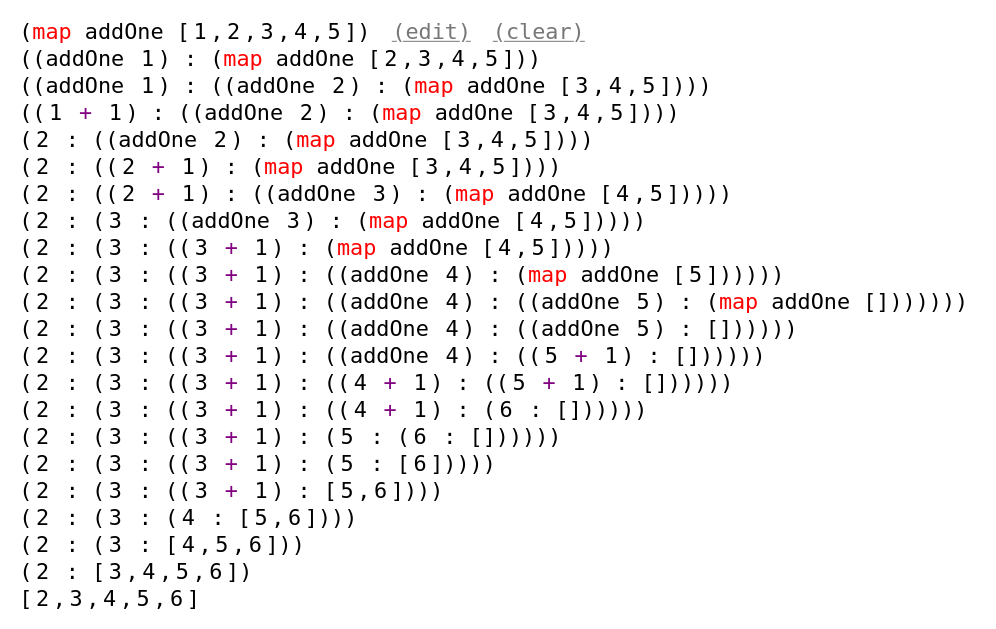
\includegraphics[width=0.75\linewidth]{images/LLessonsMap.png}
    \caption{Evaluation of\ `\sflinline{map addOne [1, 2, 3, 4, 5]}'\ with \llessons}
    \label{bg:llessons_ui}
\end{figure}

\begin{figure}[t]
    \centering
    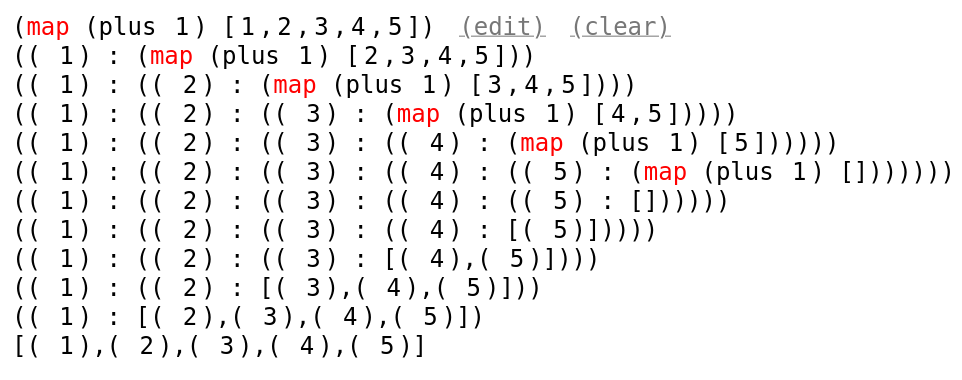
\includegraphics[width=0.75\linewidth]{images/LLessonsGoingWrong.png}
    \caption{Evaluation of `\sflinline{map (plus 1) [1, 2, 3, 4, 5]}' with \llessons. It gets confused by currying and partial application}
    \label{bg:llessons_gets_confused}
\end{figure}

The UX/UI is the definite strong point of \llessons\ (see \ref{bg:llessons_ui}).  However, there are a few things that I would identify as weaknesses that make it not useful for what SFL explorer is useful for.

\begin{itemize}
    \item The language is not typechecked. There are type assignments, but upon testing and inspection of the source code \cite{lambdalessonsgithub}, type assignments are ignored. They say on the website that the language is `dynamically typed'~\cite{lambdalessons}, but it is not. 
    \item The language does not allow for user defined algebraic data types, but it has \sflinline{List} built in. 
    \item As can be seen in \ref{bg:llessons_ui}, it seems to imply that \sflinline{((x : y : []))} reduces to \sflinline{[x, y]} which is misleading, as these two are infact identical. 
    \item The language does not support lambda functions.
    \item The language does not support currying or partially applying functions (\ref{bg:llessons_gets_confused}).
    \item The program states are not saved between refreshes. 
\end{itemize} 

\noindent In summary, \llessons\ is designed for a different purpose than SFL Explorer. It describes itself as a `document'~\cite{lambdalessons} rather than an all around teaching tool for functional languages. It does not provide much capability to experiment yourself outside of `map' and `fold' as the language is not very extensive. However, the ability to reduce an expression by clicking on the section of the expression you want to reduce is very intuitive, and inspiration could definitely be drawn from this for any future iterations of SFL Explorer. 

% \subsection{Other Notable Mentions}
% Unfortunately, I do not have the page count to spare to go into detail about some of the other existing systems identified. Here are some of my favorites, along with a brief summary of their achievements. 

% \begin{itemize}
%     \item WinHIPE \cite{WinHIPE}
% \end{itemize}

% \subsection{Conclusion of Research on Existing Systems}


% https://stevekrouse.github.io/hs.js/

\section{COMS10016: Imperative and Functional Programming at the University of Bristol}
\label{COMS10016}
In the first year of most computer science programs at the University of Bristol, students take the module \href{https://www.bristol.ac.uk/unit-programme-catalogue/UnitDetails.jsa?unitCode=COMS10016}{COMS10016}, a combined imperative and functional programming module. This is many students first encounter with both of these types of programming. In the functional part of this unit, students are taught Haskell. The unit material is presented to students through a series of lectures, supplemented by weekly worksheets that students have the opportunity to work through in labs attended by the lecturers, as well as some teaching assistants. Two of the lecturers in this unit are Jess Foster and Samantha Frohlich. 

\begin{quote}
`The aim [of the functional portion of the unit] is to introduce types and functions. Important principles include datatypes, evaluation order, higher-order functions, and purity' \cite{COMS10016}
\end{quote}

\noindent I acted as a teaching assistant in the labs for two academic years. My role was to answer students questions about functional languages or the worksheets they were given. The inspiration for this project came from my experience struggling to explain key functional programming concepts. I frequently needed to resort to writing out the evaluation sequence for a term.
\chapter{Lifecycle}
The project followed a development lifecycle inspired by Agile principles \cite{agilemanifesto2001}, structured into four iterative cycles. Each cycle was further subdivided into four phases:

\begin{itemize}
    \item Requirements Analysis. 
    \item Design
    \item Implementation 
    \item Evaluation
\end{itemize}

\begin{figure}[H]
    \centering
    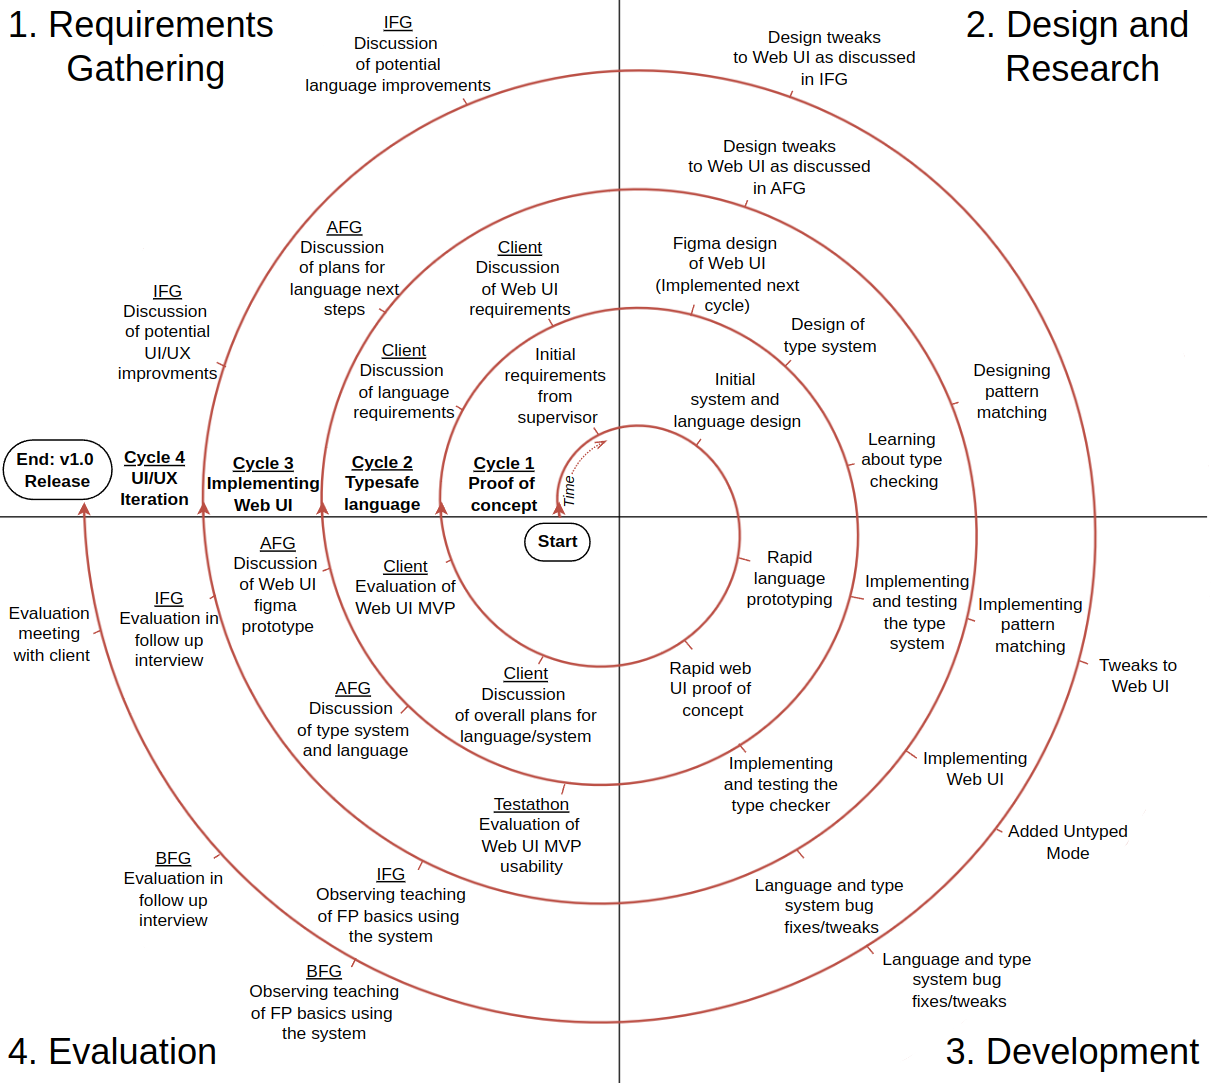
\includegraphics[width=\linewidth]{images/spiral1.drawio.png}
    \caption{Caption}
    \label{fig:spiral}
\end{figure}

In particular, the project benefitted from agile principles emphasising:
\begin{itemize}
    \item 
\end{itemize}

 
\chapter{Phase 1 --- Proof of Concept}
The goal of Phase 1, which spanned approximately the first month of my project, was to arrive at a proof of concept. This phase started at the beginning of the project with a discussion my supervisor, and the identification of my client. I proceeded by analysing the project requirements using autoethnographic methods, designing the system, designing \ac{SFL} and the Explorer, and then implementing the proof of concept. I then evaluated the merits and drawbacks of the proof of concept by speaking to my client. 

\section{Requirements Analysis}
\subsection{Autoethnography}
\label{sec:c1_autoethnography}
\begin{quote}
`Autoethnography is an ethnographic method in which the fieldworker's experience is investigated together with the experience of other observed social actors. \cite{autoethnography}'
\end{quote}

\noindent In this phase, I took an autoethnographic approach to requirements analysis and to design. As the `fieldworker', I drew on my own experience being involved in teaching Haskell for the last two academic years. This experience was very valuable to this project, and it allowed me take the initial brief from my supervisor and effectively design a solution, and then quickly implement a proof of concept of this solution. 

\subsection{The Brief}
This project was proposed by my supervisor, Jess Foster. In our initial meeting, we discussed how she wanted a tool that would help build intuition for how functional languages are evaluated, that she could use to supplement her explanation of otherwise difficult to intuit functional language concepts. We also discussed the benefits of the tool being accessible to students to use themselves during labs or at home. Jess helped me to identify an appropriate client: Samantha Frohlich. Jess and Samantha are both lecturers on \hyperref[COMS10016]{COMS10016}. It was necessary to identify a client other than Jess, as her existing role as my supervisor/primary marker could limit guidance she would be able to give me if she were also my client. 

Following this meeting, I broke down this brief into smaller parts. Taking an autoethnographic approach, I used my own experience teaching functional languages to consider solutions and come up with requirements for each part. 

\subsubsection{Building Intuition}
\label{building_intuition}
This is the key to an effective solution. \sam{MOST students OF} Many students to the first year \ac{FP} unit do not have any experience with functional programming. 
% \sam{I disagree with the rest, cos we strive for the lectures to be engaging (so maybe you can say that the teaching style is already to make learning not passive, so this will further that. Also your comment about not attending or engaging with labs is irrelevant cos if they dont engage with labs why would they use your tool? } 
\todo{REWORK THIS PARA}
and find it difficult to gain an intuition from passively watching lectures, and do not attend or engage with labs. 


% All participants who did not disagree that functional languages are hard to learn were presented with a free form text box, and asked to describe why. These responses were turned into a word cloud \ref{fig:fp_wordcloud}. Half of responses included the word `different'. 

In my experience teaching \ac{FP}, a very effective way to build intuition for functional programming languages is to demonstrate evaluation step by step. I frequently wrote out evaluations on paper for student during the \hyperref[COMS10016]{COMS10016} labs. I would also ask students to complete sections themselves. Others have also found that encouraging stepwise evaluation on paper is an effective way to get `a feeling for what a program does'. \cite{fp_first_year} [TODO: theres more things to cite here]

Thus, a tool to perform these step by step evaluations in an interactive manner would be very valuable. The tool should have an interface that allows progress to be made step by step, showing the history of past steps as well as giving information about the step about to be taken. This would allow students to understand and interact with a stepwise evaluation, without anyone having to undertake the long process of writing it out, and without risk of incorrectness. Furthermore, the effects of changing the input program could be seen quickly, providing instant feedback. 

\subsubsection{Use as a Lecture Tool} The tool should be suitable for use in lectures. It should provide an interface that facilitates quality explanation of functional programming languages. The interface must be understandable, for both \ac{FP} `experts' (lecturers, advanced users) as well as people who have never seen a functional language before. The tool must also be portable, and not require a complex installation process. 

\subsubsection{Use as a Self Teaching Tool} The tool should be `self-explanatory' enough for people to use it on their own without expert help. It should be fairly intuitive, and should have all the information required to use it presented to users. The tool must also be portable, and not require a complex installation process. The less complex this tool is to use, the more people will use it. 

\subsubsection{Demonstrating \ac{FP} languages} The tool must contain, at its core, a functional language in order to demonstrate how they work. A language that is similar to Haskell would make for easier evaluation of the project, as this would match the language taught in \hyperref[COMS10016]{COMS10016}, and therefore more people at the University of Bristol will be able to engage with the language. The most Haskell-like programming language that exists (as far as I am aware) is Haskell. 

Haskell could be included in the system/required to be installed on the host machine, however creating a demonstration tool around Haskell would be difficult due to the sheer size of the language, the number of features, and the complexity of the type system. It would be better to create Haskell-like language with a strictly limited size and maximum clarity, and include this in the system. The programming language should be designed with simplicity and clarity at its heart.

\subsection{SFL Explorer}
The requirements extracted from autoethnographic methods, as well as from my initial supervisor meeting, came together to form the idea for SFL Explorer. 

The system should be a website to maximize portability. The system should include a functional programming language, as well as some sort of UI that allows a functional program in the language to be entered, and evaluated step by step in a visual manner. 

% \begin{figure}[t]
%     \centering
%     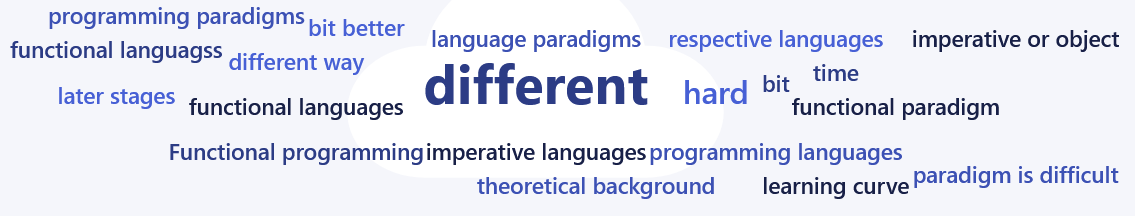
\includegraphics[width=1\linewidth]{images/fp_is_hard_wordcloud.png}
%     \caption{A word cloud of answers entered into the free form text box presented to the 10 respondents who reported that they did not disagree that functional languages were hard to learn}
%     \label{fig:fp_wordcloud}
% \end{figure}

\subsubsection{The Simple Functional Language}
\label{design:goals}
The language was given a name reflecting its core design principle: Simplicity. More precisely, the programming language should be designed with the following design principles in mind:
\begin{enumerate}
    \item \textbf{It should be simple and easy to understand}. This requires that the language should not have features that users might find difficult to understand why they work. This means that the language should have very few inbuilt functions, all of which should be easy to understand why they work. 
    \item \textbf{It should be similar to existing functional languages}. This would allow users to be able to transfer their intuition to other languages. It should be similar in syntax (it should have similar tokens and structures), as well as semantics (it should work similarly). 
    \item \textbf{It should be powerful enough to explain key concepts.}
\end{enumerate}
The features that should be selected for the language are the features that maximize these goals for the minimum implementation complexity. Out of our design goals, 2 and 3 have the potential to be in conflict, as more expressive power often requires more complex syntax. We must ensure a sensible compromise between all of our goals, while accounting for implementation complexity. When adding features for the language, we must prioritize the features that allow explanation of the `core' features of functional languages, and de-prioritise features that are not so `core' to the understanding of functional languages. 

\subsubsection{The Explorer}
The website (the explorer) should include a code editor for people to enter programs. Including the functionality for the language inside the website rather than requiring complex client/server communication would simplify the system, as well as improving responsiveness. 

[TODO: Finish this bit, summarize requirements]

\section{Language Design}
In this section, I will discuss the design of \ac{SFL} with respect to the requirements. This is iteration 1 of the design, and it was the proof of concept.  

\subsection{Definitions}

\begin{syntax}[Lowercase and Uppercase ID syntax as regular expressions]
\label{def:identifier_syntax}
(Lowercase Identifier): \(id ::= [a..z][a..zA..Z0..9\_]*\)\newline
(Operator): \(op ::= + \mid - \mid \times \mid / \mid > \mid \ge \mid < \mid \le \mid== \mid \mathrel{\mathtt{!=}} \)\newline
(Uppercase Identifier): \(Id ::= [A..Z][a..zA..Z0..9\_]*\)
\end{syntax}
\sam{im so sorry but this looks ugly. I think it just needs more space, it is very crampt, this is a minor thing and can wait till the very end}

\subsection{Basic Syntax}
Lambda calculus is the basis of modern functional programming languages. As discussed in the background, lambda calculus consists of 3 structures: identifiers, application, and abstraction. \sam{sadly this effectly says in prose the same as the BG, the only thing the BG adds is the formal definition, which not everyone will be able to read} One common extra structure that functional languages implement is an assignment. This is where we label an identifier with a certain meaning, such that all references to the assignment henceforth are identical to a reference to the meaning assigned. For instance:
\begin{lstlisting}[language=SFL]
f = (\x.x)
main = f y
\end{lstlisting}
Is identical to \sam{dont do this, cos it gives latex the chance to mess up your formatting. Always give your listings a name and use the name in a full sentence e.g. "For instance, listing 1 and listing 2 are semantically equivalent"}
\begin{lstlisting}[language=SFL]
main = (\x.x) y
\end{lstlisting}
Note the use of \verb|"\"| instead of \(\lambda\) as it is the closest character available on most keyboards. A program is then defined as a set of assignments, and we pick one specific label name to mark the `entry-point' expression in the program. Haskell, as well as many other languages, uses `main' to represent a programs' entry point, so we may use main. 

We must \sam{why must? (because we want to run our code), this is also a common extension of the STLC} also add a way to represent values, such as integers and booleans, to our language. Most programming languages, including functional ones, at least support integers. Booleans are also often supported to represent the results of integer comparison. Without literal values, programs would have to use complicated encodings (such as church numerals) to represent these values, making programs look more complicated.  \sam{bring this why forward}
\sam{this is a very typical para for you: i encourage you to structure your paras as because of x we need y, instead of we need x because of y}
\sam{no new line}
These two features massively shorten and simplify programming in this language.

\sam{this is not referenced anywhere. Above you say we need x and then just dump x here. Instead motivate, introduce and explain. What additions have been made to execute x. Explain your definitions like you would explain your code}
\begin{syntax}[The basic syntax of \ac{SFL}]
(Expression) \(E, F ::= [-][0, 1, ..]\mid E\; op\; F \mid true \mid false \mid id \mid \setminus id. E \mid E\:F\)\newline
(Assignment) \(A ::= id = E\)\newline
(Module) \(M ::= A\: M \mid End\)
\end{syntax}

\subsection{Reduction and Progress}
\label{c1_design_reduction_progress}
As discussed in the background, functional programs progress via reduction. \ac{SFL}  programs can reduce when we have an abstraction applied to a term. 

We may also want to replace variables with their assigned values. This is not reduction, however it is still progress

\todo{FINISH, will be easier when the bg on reduction is improved}

\section{Implementation}
\subsection{The Abstract Syntax Tree}
The tree structure of \ac{SFL} requires the following different types of tree nodes:
\begin{itemize}
    \item Identifier
    \item Literal
    \item Pair
    \item Application
    \item Abstraction
    \item Match
    \item Assignment
    \item Module
\end{itemize}
\sam{bullets look silly, if you have spare time draw a pictures, otherwise just say that it is a tree structure, listing the nodes adds nothing}

Initially, the approach taken when implementing this tree structure was to have each node `owning' its child nodes (see \ref{bg:rust}). However, it will be frequently necessary to be able to find nodes based on certain conditions (for example, the condition that this node is a valid redex) and then provide a value that represents the location of this node within the tree. Even if each of the tree nodes had a unique ID, locating a node from this value representing its location will require some sort of tree search.

Rather than this solution, which would have a non-constant node lookup time, a secondary structure can be used to store the tree nodes with constant time lookup, and then each node can store a value enabling constant time lookup of its children within this structure. In the implementation, these types were labelled as \ac{AST} and ASTNode, where \ac{AST} was an array of ASTNodes, and each ASTNode stored their children's indices in this array. The position in the array of an ASTNode will be referred to as its index.

\begin{figure}[t]
    \centering
    \begin{tabular}{c}
    \hline
    \begin{lstlisting}[language=Rust]
struct AST {
    vec: Vec<ASTNode>,
    root: usize,
}

enum ASTNodeType {
    Identifier,
    Literal,
    Pair,
    Application,
    Assignment,
    Abstraction,
    Module,
} 

struct ASTNodeSyntaxInfo {...}

struct ASTNode {
    t: ASTNodeType,
    token: Option<Token>,
    children: Vec<usize>,
    line: usize,
    col: usize,
    type_assignment: Option<Type>,
    additional_syntax_information: ASTNodeSyntaxInfo
}
    \end{lstlisting}
    \\\hline
    \end{tabular}
    \caption{The Rust code listing for the definition of the AST, with lifetime specifiers, accessibility modifiers, and the syntax information (see \ref{paragraph:to_string}) removed for conciseness.}
    \label{fig:ast_lst}
\end{figure}

See \ref{fig:ast_lst} for the code listing for the \ac{AST} definition. In this implementation, \verb|Vec| was used for the array, as it is growable, resizeable, and facilitates constant-time lookup of its elements. The \ac{AST} stores and owns all of the nodes, as well as storing the index of the root node rather than requiring it to be at a specific index. 

The node indices in the \verb|children| vector represent different things depending on what kind of node it is. 
\begin{itemize}
    \item If it is an abstraction, the first node represents the variable (or pair of variables) abstracted over, and the second node represents the expression.
    \item If it is an application, the first node is the function, and the second is the argument.
    \item If it is a pair, the first node is the first in the pair, and the second is the second in the pair.
    \item If it is a match expression, the first node represents the matched value, then after this it consists of the case followed by the resulting expression. Match expressions will always therefore have an odd number of children.
    \item If it is a module, then each of the children is an assignment.
    \item If it is an assignment, then the first child is the variable being assigned to, and the second is the expression.
\end{itemize}

\verb|Literal| and \verb|Identifier| nodes store the tokens that defined them, so the strings can be accessed. \verb|Identifier| nodes used as abstraction arguments. These types can either be specified in the source program, or inferred later. Nodes also store their positions (line and column) in the source program, which can be used for error messages. 

In order to effectively explain the structure of a parsed program going forwards, the following structure will be used to give a written representation of an AST:
\begin{itemize}
    \item Nodes are represented as one line each, where, with the name of the node type, followed by its value for \verb|Literal|s and \verb|Identifier|s.
    \item The children of a node are all of the nodes with an indentation level one deeper than the node in question listed directly below it, until a shallower or equal depth node is listed. 
\end{itemize}

\noindent
For instance, 
\begin{lstlisting}
main = (\x.1) 2
\end{lstlisting}
would be represented as:
\begin{lstlisting}
Module:
  Assignment:
    Identifier: main
    Application:
      Abstraction:
        Identifier: x
        Literal: 1
      Literal: 2
\end{lstlisting}

\subsubsection{With the Benefit of Hindsight} % for jess's benefit as she did not like my AST definition so i want to aknowledge what she said about it
\sam{very nice evaluation, love this section}
This project was my first major project using Rust. Below is a discussion of some Rust features which were not fully taken advantage of in this definition of syntax trees, followed by a discussion of the combination of these features that would have been more optimal. 

\paragraph{Tagged Unions}
An alternative implementation could have involved \verb|ASTNodeType| being a tagged union, with different node types being associated with different children and data items. For instance, application could be represented by \verb|Application(f: usize, x: usize)|, and identifiers could be 

\noindent\verb|Identifier(String)|. This would be more space efficient, as each node requires different data. It would also more elegantly represent the fact that each type of node is a different thing, and de-obfuscate the meaning of each of the different fields of a node. 

\paragraph{References}
This definition of the \ac{AST} \sam{i dont understand the rest of the sentence} and the nodes has a parent object owning all of the nodes. As previously discussed, this was done to enable constant-time lookup of nodes from their indices. However, all things in a program already have such a reference enabling constant time lookup: a pointer, represented in rust by a reference. This was not used, as there were concerns about ensuring validity of each reference, and avoiding use-after-free bugs. These concerns were unfounded, as one of Rust's major features is that it provides safety guarantees ensuring that these problems are never encountered \cite{rust_book}. An object can only store a reference to another object if it can be guaranteed that it exists, and it will continue to exist for at least as long as the object storing the reference will. This is achieved via lifetime checking, using either inferred or explicitly stated specifiers of how long the two objects will exist relative to each other. 

\paragraph{A Better Implementation}
\sam{numbers alone look odd, especially at the beginning of a sentence. An easy solution is to always give references titles e.g. Figure bla or Table bla}\ref{fig:ast_lst_2} shows an implementation that uses tagged unions to store information that is different for different node types, and pointers to the nodes directly rather than list indices. This avoids the possibility of referencing nodes that don't exist. It is also easier to understand what is common between nodes (syntax info) and what is uncommon. It is also more space efficient as it only stores the information that each type requires. The size of the improved implementation is 88 bytes, and the size of the original implementation is 128 bytes. The improved implementation is subjectively more elegant and readable. Objectively, it also takes up less space. It also forces memory safety, without the need for carefully implemented getter and setter functions. 

Despite this, the decision was made not to update the implementation for several reasons. The \ac{AST} is so central to the implementation, that it would take a long time to switch properly. Memory and speed are not major constraints for this project, but implementation time is. Furthermore, as long as all indices used are either produced by a helper function, or the \ac{AST} root, there should not be a problem with memory safety. 

\begin{figure}[t]
    \centering
    \begin{tabular}{c}
        \hline
    \begin{lstlisting}[language=Rust]
struct AST<'a> {
    vec: Vec<ASTNode<'a>>,
    root: &'a ASTNode<'a>,
}

enum ASTNodeType<'a> {
    Identifier{name: String},
    Literal{value: String, _type: PrimitiveType},
    Pair{first: &'a ASTNode<'a>, second: &'a ASTNode<'a>},
    Assignment{to: String, expr: &'a ASTNode<'a>, type_assign: Type},
    Abstraction{var: String, expr: &'a ASTNode<'a>, type_assign: Type},
    Module{assigns: Vec<&'a ASTNode<'a>>},
    Match{expr: &'a ASTNode<'a>, cases: Vec<&'a ASTNode<'a>>}
} 

struct ASTNodeSyntaxInfo { ... }

struct ASTNode<'a> {
    t: ASTNodeType<'a>,
    info: ASTNodeSyntaxInfo
}
    \end{lstlisting}
    \\\hline
    \end{tabular}
    \caption{An alternative implementation with a few advantages over the actual implementation. }
    \label{fig:ast_lst_2}
\end{figure}

\subsection{Methods on the AST}
Below are a selection of the more important or interesting methods implemented on the \ac{AST} and its nodes. \sam{i think I want to see the code as well}

\paragraph{Adding new nodes} We will frequently want to add new nodes to the tree. Where they are inserted is not important, so the tree will add them to the end, and return their index. These methods are needed extensively for the parser.

\paragraph{Getting children of nodes} As the interpretation of the \verb|children| array for each node changes depending on what type of node it is, a series of getters are implemented, such as `\verb|get_func|' to get the function of an application. These methods are needed extensively for the type checker, and the redex finding system. 

\paragraph{Substitute variable} Substitutes all instances of a variable in an expression with a given expression. This is needed for applying abstractions. For instance, the process of reducing \verb|(\x.x) 1|, is:
\begin{itemize}
    \item Get the name of the variable abstracted over: \verb|x|.
    \item Replace all instances of x in the abstraction expression with the right hand side of the application: \verb|1|.
    \item Replace all references to the abstraction with references to the abstractions expression. 
\end{itemize}

Note that this orphans the node for the abstraction, and the node for the abstraction variable \verb|x|. This is hard to rectify as deleting any nodes will shift the whole list, which would invalidate indies of nodes, which will break many of the references. This is rectified by cloning the AST, as described below.

\paragraph{Clone} The AST, or just a subsection of the \ac{AST} from a given node, can be cloned by starting from the desired new root, and cloning each nodes children recursively. The new indices of each node may not be the same, as they may be moved in the list, but they will all be in the same place relative to each other. This also removes orphaned nodes, as they will never be cloned as they have no parents. 

\paragraph{To String} \label{paragraph:to_string} Programs can also be effectively transformed back into strings. This requires a few other pieces of information to be associated with some tree nodes, to make the output program as similar to the input program as possible. The more similar the output is to the input, the easier it is to understand. Some examples include:
\begin{itemize}
    \item Whether the application was generated by using the right associative \verb|$| operator in order to avoid parenthesis, for instance \verb|id $ 1 + 1|. 
    \item Whether the assignment, where the expression is an abstraction, was generated using the syntax \verb|x = \a.e| or the syntax \verb|x a = e|. 
\end{itemize}
We must also take into account whether a binary infix operator was used to generate a function call, and if so we must place it in the middle of its arguments. 

% There is also other syntax sugar, such as turning a List from `Cons' syntax into more familiar braced syntax, with comma separation.   For instance: \verb|Cons 1 (Cons 2 (Cons 3 Nil))| should be displayed as \verb|[1,2,3]|. [TODO: Consider whether to have only literals in this syntax or everything. Maybe toggleable syntax sugar?]

\subsection{Finding Redexes}
\todo{do once the background is fixed}
In SFL, a redex is an application \sam{unfinished?}

\subsection{The Parser}
The parser needs to consume a program, and return the following things:
\begin{itemize}
    \item The AST.
    \item The `Label Table': The types of all labels defined, including both those defined explicitly (assignments) or implicitly (constructors). This is implemented as a struct `\verb|LabelTable|' which is a wrapper around a \verb|HashMap<String, Type>| with some useful methods. 
    \item The `Type Table': All type constructors and concrete types defined, stored with their arities. This is implemented as: \verb|HashMap<String, usize>|.
\end{itemize}
For instance, from the program: \sam{examples are good!}
\begin{lstlisting}[]
data List a = Cons a (List a) | Nil
double x = x * 2	
main :: List Int
main = Cons (double 1) (Cons (double 2) Nil)
\end{lstlisting}
We should extract the following data:
\begin{itemize}
    \item The AST: 
    \begin{lstlisting}[]
Module:
  Assignent
    Identifier: double
    Abstraction
      Identifer: x
      App
        App
          Identifier: +
          Identifier: x
        Literal: 2
    \end{lstlisting}
    \item All the known type assignments (excluding inbuilts)
        \begin{itemize}
            \item Cons: \(\forall a. a \Rightarrow List\;a\Rightarrow List\;a\)
            \item Nil: \(\forall a. List\;a\)
            \item main: \(\forall a. List\;a\)
        \end{itemize}
    \item The names of all known types (excluding inbuilts) 
        \begin{itemize}
            \item List, with an arity of 1
        \end{itemize}
\end{itemize}

% \sam{some advice i got when i started technical writing, as i think you are writing very similarly to  how I used to: when writing a report it is tempting to well report "this was done" "that was done" "this means" "noun will need to" but this results in quite dry and overly verbose writing. Instead it is more exciting to make the research / the noun the subject of the sentence. e.g. "noun needs to bla because of bla"}
The parser will also store a set of all bound variables at each location. This will allow us to disqualify some invalid programs while generating the tree, rather than having to traverse it after generation to catch these issues. For instance, we must the following assignments:
\begin{itemize}
    \item \verb|x = (\x. e)| where e is a valid expression, as x is ambiguous during the expression e. This would be disqualified when attempting to parse the abstraction as x is already bound.  
    \item \verb|x = y| where y is undefined.
\end{itemize}

\subsubsection{Lexical Analysis}
Lexical analysis is the process splitting a program into its constituent tokens (Lexemes). For instance, the program \verb|main = (\x.x) 1| is the following stream of tokens: \[[Id: main, Assignment, LeftParen, Backslash, Id: x, Dot, Id: x, RightParen, Literal: 1]\]
See \ref{appx:tokens} for the code listing of the definition of the tokens output by the lexical analysis.

The lexer loads the entire string into memory at once. This is not typical, as this can lead to problems with large files. The approach discussed in \cite{dragon_book} relies on a system of two buffers only holding individual pages of the file from disk. However, this system will not be loading files from disk; the program string is already in memory as it comes from the UI. Therefore, there would be no benefit to a more traditional lexer optimised to reduce memory usage. 

The lexer provides a \verb|next_token| function that returns the next token, and advances the pointer to the start of the token after. The lexer keeps track of line and column information, which is stored in the token to then be stored in the AST. 

\subsubsection{Expression Parsing}
Expressions are parsed using recursive descent parsing. Some of the techniques used for this part of the parser were inspired by the discussion of top down parsing in \cite{dragon_book}. 

At the top level, the expression parsing method is \verb|parse_expression|. A variable \verb|left| stores what is currently the index of the expression. It is called \verb|left| as if we encounter a token that denotes that \verb|left| is applied to whatever comes next, it becomes the left hand side of the application. \verb|left| is originally set to be the output of parsing a primary (see \ref{impl:parsing_primary}), and then progresses differently based on the next token.  Below are some of the ways that \verb|parse_expression| could proceed.
\begin{itemize}
    \item If the next token is an open bracket, we consume the token and then parse an expression. We then expect a closing bracket. We set \verb|left| to the application of \verb|left| to the expression
    \item If the next token is a dollar sign, we consume the token and then parse an expression. We do not expect a closing bracket, and we error if we receive one. We set \verb|left| to the application of \verb|left| to the expression.    
    \item If the next token is a token denoting the start of a primary expression structure:
    \begin{itemize}
        \item A backslash, indicating the start of a lambda
        \item An identifier, indicating a variable.
        \item A literal
    \end{itemize}
    We parse a primary, and set \verb|left| to the application of \verb|left| to our primary.
    \item If the next token is:
    \begin{itemize}
        \item A closing bracket
        \item EOF
        \item A newline
        \item An opening brace (indicating the end of parsing the matched expression of a match statement)
        \item A double colon, indicating a type assignment follows
    \end{itemize}
    We return \verb|left|. 
\end{itemize}

\paragraph{Primary Parsing}
\label{impl:parsing_primary}
A primary is a less complex structure than an expression. In this system, a primary is any expression structure other than applications. The primaries are:
\begin{itemize}
    \item Literals
    \item Identifiers
    \item Lambdas
    \item Expressions in brackets
\end{itemize}
Each of these have their own specific parsing algorithms, which may include calling \verb|parse_expression|. 

\paragraph{Literal and Identifier Parsing}
Literals and identifiers are turned trivially into their respective AST Nodes. For instance, the token:
\begin{verbatim}
Token {
    line: 0,
    col: 0,
    tt: TokenType::IntLiteral
    value: "2"
}
\end{verbatim}
Is turned into this ASTNode:
\begin{verbatim}
ASTNode {
    t: ASTNodeType::Literal,
    token: Some({the token}),
    children: [],
    line: 0,
    col: 0,
    type_assignment: Option<Primitve::Int>,
    additional_syntax_information: ...
}
\end{verbatim}

\paragraph{Parsing Abstractions}
Abstractions (in the simple case) are parsed by:
\begin{itemize}
    \item Consuming a lambda (represented by `\verb|\|' for ease of typing on standard keyboards)
    \item Parsing a variable. This variable must be added to our set of `bound' variables.
    \item Consuming the dot separator`\verb|.|'
    \item Parsing an expression
    \item Constructing an abstraction node from the variable and the expression
\end{itemize}

However, the definition of abstractions has a few complicating elements of syntax sugar.

\subparagraph{Abstractions May be Assignments}
The assignment \verb|f x = x| is implicitly \verb|f = \x. x|. This is solved by parsing an argument to \verb|parse_abstraction| representing whether this is an assignment. If it is an assignment, we do not parse the lambda, and expect the assignment operator `\verb|=|' as our separator rather than the dot. As previously mentioned in\ref{paragraph:to_string}, in order to output the string in a format that is as close as possible to the input, we set a flag in the \verb|ASTSyntaxInfo|: \verb|assign_abst_syntax| to all abstraction nodes defined like this. 

\subparagraph{Abstractions May Have Multiple Variables}
The abstraction \verb|\x y. x| is syntax sugar for \newline\noindent\verb|\x. (\y. x)|. Additionally, with the assignment syntax, \verb|f x y = x| is syntax sugar for \newline\noindent\verb|f = \x. (\y. x)|. This can be accounted for by continually parsing variables until we encounter `\verb|.|' or the assignment operator `\verb|=|', and then producing a series of abstractions over these variables in order. 

To parse an identifier, we must also check that the identifier is bound at this location.

\subsection{Web UI \ac{MVP}}
As part of this section, I also developed the MVP for the Web UI. \ref{fig:screenshot_phase_1_end} shows the web UI after this stage of the project. 

\begin{figure}[h]
    \centering
    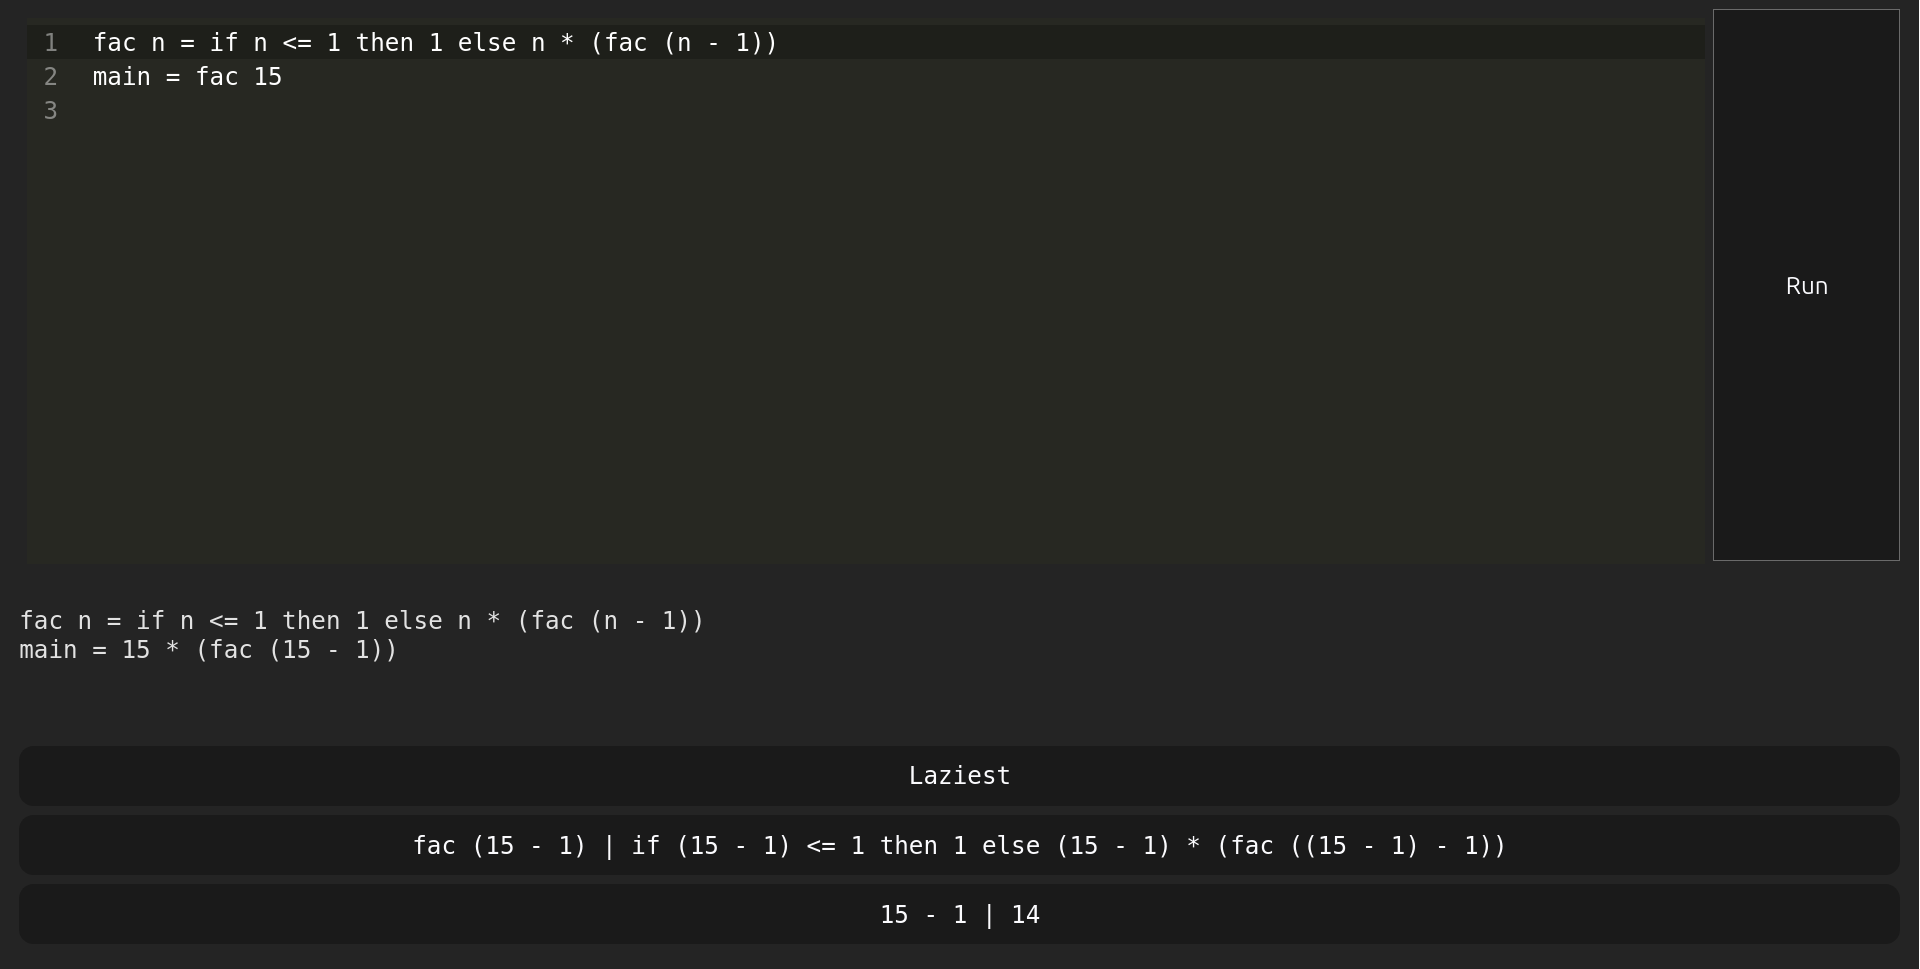
\includegraphics[width=1\linewidth]{images/phase-1-end.png} 
    \captionsetup{justification=centering}
    \caption{The Web UI \ac{MVP}, as presented to my client at the end of phase 1.}
    \label{fig:screenshot_phase_1_end}
\end{figure}

Until this point, development was done in one rust package. This package would be compiled to a binary and run natively, with a basic \ac{CLI}. This needed to be changed so that it can compile to \ac{WASM} and run in the web browser. As I wanted to keep the \ac{CLI} for debugging, as well as for use later, I did not want to change the whole project to a project with a \ac{WASM} interface. A solution to keeping both interfaces was to separate the functionality that would be common to the \ac{CLI} as well as the \ac{WASM} library into a separate library, and then have the two interfaces as separate packages that depended on this one. The structure of the project became the following 4 packages. 

\begin{itemize}
    \item \textbf{libsfl}: All of the language functionality, as this is common to both interfaces
    \item \textbf{sflcli}: All of the original CLI functionality without the language functionality.  
    \item \textbf{libsfl\_wasm}: a package set up for use with wasm-pack (\ref{bg:wasm-pack}). It provides a wrapper around \textbf{libsfl}, with wrapper functions returning data structures supported by wasm-bindgen\ref{bg:wasm-bindgen}. wasm-pack would compile this to an \ac{NPM} package containing:
    \begin{itemize}
        \item The WASM binary blob of the compiled rust code
        \item A JavaScript file that would load the blob into the browsers' memory, and provides methods that can call the appropriate the methods in the blob
        \item A TypeScript file providing the types of all of the packages exported functions. 
    \end{itemize}
    \item The Vite+React frontend (see \ref{bg:frontend}) that requires the package that results from compiling \textbf{libsfl\_wasm}
\end{itemize}

The \ac{WASM} library provided functions that could be called from the JavaScript module. Rather than passing the \ac{AST} around between the \ac{WASM} library and the JavaScript module, the \ac{AST} was stored in


\todo{original approach was to use a set memory region for the AST as i did not wanna pass it to javascript}


[TODO: More stuff about WASM bindings??]

\section{Proof of Concept Client Meeting: Evaluation and \newline Next Steps}
\label{eval:c1}
At the end of the phase, I presented the proof of concept project to my client, who was very positive about the project and its potential. The discussion was informal, a friendly conversation rather than a structured interview, to allow the direction of questioning to change depending on the clients answers. The meeting started with me giving my client a demo of the proof of concept using by using the system to evaluate the following program:
\begin{verbatim}
fac n = if n <= 1 then 1 else n * (fac (n - 1))
main = fac 5
\end{verbatim}

Below is a summary of my clients thoughts about various aspects of the proof of concept system and potential future iterations

\subsection{Usefulness as a Teaching Tool}
Below are some notes on what the client thought about the effectiveness of the project as a teaching tool, and how it could be improved in future iterations.
\begin{itemize}
    \item The project is already very useful as a teaching tool to demonstrate:
    \begin{itemize}
        \item Evaluation order, and the importance of laziness
        \item Currying
        \item Recursion
        \item The \lcalc
    \end{itemize}

    \item On top of this my client wanted to be able to use the system to demonstrate: 
    \begin{itemize}
        \item High Priority
        \begin{itemize}
            \item List and common list functions such as `map' and `fold'. These do not have to by polymorphic, they could be just defined over $Int$s or some other type. These also do not need to be user-definable, they can be built in. 
            \item Pattern Matching
        \end{itemize}
        \item Lower Priority 
        \begin{itemize}
            \item User definable data types, preferably polymorphic. This would mean we could define `$List$' as part of the language which would be good for clarity. 
        \end{itemize}
    \end{itemize}
\end{itemize}

\subsection{The Existing Language}
\paragraph{Positives:}
\begin{itemize}
    \item The language looked similar to Haskell. Particularly, the \verb|if _ then _ else| syntax, and the function assignment shorthand syntax (\verb|fac n = ...| rather than \verb|fac = \n. ...|, even though these are identical)
    \item The language is minimal and clear
    \item The factorial function was quite elegant, and it would be understandable to people who did not know Haskell.  
\end{itemize}

\paragraph{Negatives:}
My client had no specific complaints about the language as it currently stands, however we agreed was lacking many important features. The most difficult things to teach are concepts involving more complex data types. 

\paragraph{Requested Features:}
Below are the specific features my client asked for in order for the system to be able to demonstrate the things she wants to use the system to demonstrate:
\begin{itemize}
    \item Recursive Types
    \item Polymorphism
    \item Type Aliases
    \item Typechecking
    \item User Definable Data Types
\end{itemize}

\subsection{The Existing UI/UX}
\paragraph{Positives:}
\begin{itemize}
    \item The editor, as it feels like a very popular editor: VSCode
\end{itemize}

\paragraph{Negatives}
\begin{itemize}
    \item It is unstable. This is bad in a teaching tool, as it would waste a lot of time if it constantly broke in the lecture. 
    \item `laziest' as an option is confusing, as it was unclear if it was referring to one of the other on screen options, or if it was referencing a `hidden' option
    \item The vertical bar separating redex from contraction on the progress buttons was not obvious enough. On top of this, the bar was not centred, so it was hard to look through all the redexes at once as they were not aligned with each other. 
\end{itemize}

\paragraph{Requested Features}
\begin{itemize}
    \item Syntax highlighting, to make the language easier to read   
    \item A history of what the expression has been is vital to demonstrate step by step evaluation. I identified this as an important feature at the beginning of the phase (see \ref{building_intuition}), but I had not finished it by the client meeting. It was implemented in the next phase (see \ref{c2_poc_ui_impl}). 
    \item Sample Programs
\end{itemize}

\subsection{Conclusion}
At the end of this phase, and going into phase 2, I had a strong proof of concept system and an idea for how the system will look. The meeting with my client yielded many ideas, all of which I sucessfully implemented throughout this project. 
\chapter{Phase 2 --- Types and Pattern Matching}
In this phase, I moved away from the autoethnographic (\ref{sec:c1_autoethnography}) approach, where most of my requirements came from within, to an externally motivated approach where my requirements came from my client. This phase was mostly focused on adding more features to \ac{SFL}, including a polymorphic type system and pattern matching. 

% \sam{dont bother changing this for this project, this is just advice for future: this section would read much better if for each proposed change you did: motivation for change, details of change, implementation of change, eval of change. Each per change. It reduces what the reader has to remember and stops you need to repeat yourself so much}

% At the end of this phase, I held a focus group (\ref{ref:afg}) to help me evaluate the progress of the project. Because this was the plan from the beginning of the phase, 

\section{Requirements Analysis}
The requirements for this phase were motivated by my client meeting~(\ref{eval:c1_client}). 
The client's central idea for what they wanted to use the tool was to demonstrate methods on lists, such as `map' and `foldr/l'. Lists in functional programming languages are commonly defined recursively, using \verb|Cons x xs| to represent constructing a list from an element \verb|x| and the rest of the list \verb|xs|. \verb|Nil| represents an empty list. This recursive construction of lists comes from Lisp \cite{mccarthy1960recursivelisp}. Similarly, in Haskell, lists are defined as follows:
\begin{lstlisting}[language=SFL]
data [a] = [] | a : [a]
\end{lstlisting}
This definition of lists is as example of a polymorphic data type. It also implicitly defines two polymorphic constructors, \verb|[]| (Nil) which has type $\forall a. [a]$, and \verb|:| (Cons) which has a type $\forall a. a \fto [a] \fto [a]$. 

In order to support recursively defined Lists like this in \ac{SFL}, we could either have `Nil' and `Cons' built in, or we could allow them to be defined in the language. Providing a mechanism for users to define their own types in the language, including lists, would be the best option as this would allow maximum clarity and transparency into how the language works. 



% Allowing them to be defined in the language would be best for clarity, and it would also allow users 


% I wanted to tackle the most technical aspects in this phase to give me the maximum time to complete them, as this was still early in the project lifecycle. 


\section{Design}
\subsection{Language Changes}
The focus of this project phase is mainly to upgrade the language. We have already identified what features we would like to add the language. This section will go into detail about the design for the extension for the language enabling these new features. 
\subsubsection{Type System}
\label{sec:type_system_design}
% \sam{ive thought further about this, i still agree with what i said, but i think the reason this section suffers is that updates to the types needs to come LAST}
% \sam{this para could be much cleaner. If I am right, by this point we have established what is going to be added in this phase and why, this is just about noting how that will effect the type system. (if you want to keep your prose that reminds the reader what if being added and why, that is fine, but put it BEFORE you start talking about types) So the para could run: the extensions to the language, naturally led to extensions of the type system. Here is how each language extension needs supported by extensions to the type system: (use bullets if each extension only takes one or two lines, use paragaph formatting if its more like para) adding bools and ints - clearly Int and Bool types must also be added ...}
If we are to effectively represent the type of expression containing integers and booleans, we must have types $Int$ and $Bool$. We also want our type system to be able to express functions, as our language support functions. We also want polymorphism in our type system, as rewriting functions many times for different data types makes programs more verbose.  

% \sam{clunky sentence}
Allowing for algebraic user defined data types similarly to Haskell would make the language much more expressive and much more powerful, as well as bringing it closer to Haskell. Supporting tagged unions and tuples in the \ac{SFL} type system would massively increase the ease of writing complex programs. It would also allow for complex data structures such as trees and lists. 

Type names, as well as constructor names,  start with uppercase letters in Haskell. This allows them to be easily differentiated from type variables, as well as regular variables.

First-order polymorphic type constructors would be useful to have in \ac{SFL}, with one example of their utility being defining the polymorphic function `\verb|length :: List a -> Int|' which should work regardless of what type the list is over. 

% \begin{figure}[h]
  \centering
  \[
      \begin{array}{llcl}
      \text{Types} & A, B, C & \bnfas &
            \Inttype \bnfalt \Booltype \bnfalt \alpha \bnfalt 
            \alltype{\alpha}{A} \bnfalt A \arr B \bnfalt
            % \\[1pt] &&&\!\!\!\;\; \TypeAlias{A}{B} \bnfalt  
            (A, B) \bnfalt
            \Unionname[A_1, \dots, A_n]
      \\[2pt]
      \text{Monotypes} & \tau,\sigma & \bnfas &
            \Inttype \bnfalt \Booltype \bnfalt \alpha \bnfalt \ahat \bnfalt 
            A \arr B \bnfalt (A, B)
            % (A, B) \bnfalt \TypeAlias{A}{B}
        \\[2pt]
      \end{array}
  \]
  
  \captionsetup{justification=centering}\caption{Syntax of types and monotypes. Note that this is the external definition: as seen by the users of SFL. See \ref{fig:tc_types} for the extra type system structures required internally for the typechecker}
  \FLabel{fig:alg-syntax}
\end{figure}

\begin{figure}
    \[
        \begin{array}{llcl}
            \text{Types} & A, B, C & \bnfas &
                Int \bnfalt 
                \Booltype \bnfalt 
                \alpha \bnfalt \alltype{\alpha}{A} \bnfalt 
                A \arr B \bnfalt (A, B) \bnfalt \Unionname[A_1, \dots, A_n]
            \\[2pt]
        \end{array}
    \]
    \caption{The SFL type system. }
    \label{fig:sfl_types_no_exst}
\end{figure}
% Note that our type constructor application definition above is more permissive than is correct, as it does not enforce correct arity. This can be handled by the parser maintaining the context of the arity of each type, which can check that it is saturated before 

\subsubsection{User Definable Algebraic Data Types}
\label{c2:design_data_types}
In Haskell, we can create algebraic types using the \sflinline{data} keyword (see \ref{bg:haskell_udt}). Replicating this syntax for \ac{SFL}'s user defined data types is desirable because it would allow people already familiar with Haskell to use the system, as well as viva versa. 

As an example, the SFL (and Haskell) data declaration:
\begin{lstlisting}[language=SFL_noprelude]
data Either a b = Left a | Right b
\end{lstlisting}
% \sam{breaking sentences up with code or pictures is a huge formatting bug bear for me. I won't comment on this again, and it can stay if you don't have time, but if you do have time it will add a more polished and professional feel. The change needed would be something along the lines of. "As an example, we seek to support the following data declaration, exactly copying Haskell's syntax: ~code~ This declaration creates ..."}
\noindent creates a tagged union type called $Either$ with two constituent type parameters $a$ and $b$. In our type system (\ref{sec:type_system_design}) this would be represented as $Either[a, b]$. The \Unionname 
 \ \verb|Either| uniquely identifies this type, this must be enforced by the parser. It also creates two data constructors: \verb|Left| which has the type $\forall a\;b. a \fto Either[a,b]$, and \verb|Right| which has the type $\forall a\;b. b \fto Either[a,b]$. 

Type aliases allow us to make code more readable and expressive. For instance, if we were to define playing cards like this:
\begin{lstlisting}[language=SFL]
data Suit = Hearts | Clubs | Spades | Diamonds
data Rank = Num Int | Jack | Queen | King | Ace
type Card = (Suit, Rank)
\end{lstlisting}

\noindent having the type alias \sflinline{Card} for \sflinline{(Suit, Rank)} allows us to very easily, and more readably, create functions on Cards, as well as values with that type. 

To summarize, we will implement type aliases and algebraic data types that work similarly to Haskell with similar syntax. % \sam{type aliases feel out of the blue}

\subsubsection{Match}
\label{c2_design_match}
% \sam{one sentence reminder to reader of what patternmatching is: "Pattern matching is an elegant form of branching used in many functional languages." (this just sets the scene better)}
Pattern matching is an elegant form of branching used in many functional languages. Here is basic example of pattern matching in Haskell: 
% \sam{the preceeding sentence sounds very weird because it has no subject. You either want to say "fac is a basic example" or "here is a basic example"}

\begin{lstlisting}[language=SFL]
fac :: Int -> Int
fac 0 = 1
fac n = n * fac (n - 1)
\end{lstlisting}

\noindent Here, the definition of the `fac' function is different depending on if is it applied to $0$ or to any other $Int$. If it is applied to an $Int$ other than 0, n is substituted for this value in the expression.  See \ref{bg:haskell_pattern_match} for more information about Haskell pattern matching. 

\paragraph{Syntax}
Pattern matching at the top level like this would be difficult to implement, as it would require significantly changing how abstractions are represented. It would be simpler to create a new syntax structure: a match expression. This could look like:

\begin{lstlisting}[language=SFL]
fac :: Int -> Int
fac n = match n {
    | 0 -> 1
    | _ -> n * (fac (n - 1))
}
\end{lstlisting}
This syntax was fairly arbitrary, as syntax is quite easy to change. However, this syntax proved to be fairly popular with all three focus groups, so it did not change between this stage and the end of the project. 

The `fac' function takes an $Int$ n, and proceeds differently with different values of n. If the value is 0, the value of the whole expression becomes 0, otherwise it becomes \lstinline[language=SFL]!n * (fac (n - 1))!. We can use literals in our pattern to differentiate between different values of literals. Inspired by Haskell, we can use a variable (which is a lowercase identifier) to match anything, a `wildcard' pattern. All instances of the variable in the pattern's corresponding expression with the term that the variable matches. `\_' is a special case wildcard, where no variable is bound, but it still matches anything, 

We should also be able to match more complex structures including Algebraic Data Types. For instance, we can write the following function to figure out whether a list has length 2 or grater

\begin{lstlisting}[language=SFL]
lenIsAtLeastTwo :: List a -> Bool
lenIsAtLeastTwo list = match list {
    | Cons _ (Cons _ _) -> true
    | _ -> false
}    
\end{lstlisting}

\noindent In the above example where we defined `lenIsAtLeastTwo', when attempting to pattern match, it is important that we evaluate the term `list' enough to \textit{know for sure} that it does not match the first pattern before moving on to the second, as the second pattern is irrefutable. 

\paragraph{Reduction and Progress}
\label{c2_design_match_progress}
In the previous iteration of the language design, we discussed the two types of progress in \ac{SFL}: $\beta$-reduction and substitution. In order to support pattern matching, we add a third type of progress representing succeeding in pattern matching. 

\subsection{Next UI Iteration}
\label{c2:next_ui}
At this phase of the project, the current version of the web UI is a proof of concept. See \ref{fig:screenshot_phase_1_end} for the current state.

I completely redesigned the UI based on the clients' feedback, as well as based on other requiremenets identified during the \hyperref[sec:c1_autoethnography]{autoethnographic} phase of the project.  See \ref{fig:screenshot_figma1} and \ref{fig:screenshot_figma2} for screenshots of the new design. 
% \sam{talk about these designs! This section is very thin, you just say heres what im aiming for, totally chatted to focus group, but the reader will be interested in why you went this way and what the focus group said. This is more reason I suggested at the top to tackle each change one by one cos you're always leaving the reader hanging and pointing else where in the document, but it is not dramatic suspense, I'm just opening more tabs in my brain than I can cope with}
These designs were done using \href{https://figma.com}{Figma}. 

\begin{figure}[h]
    \centering
    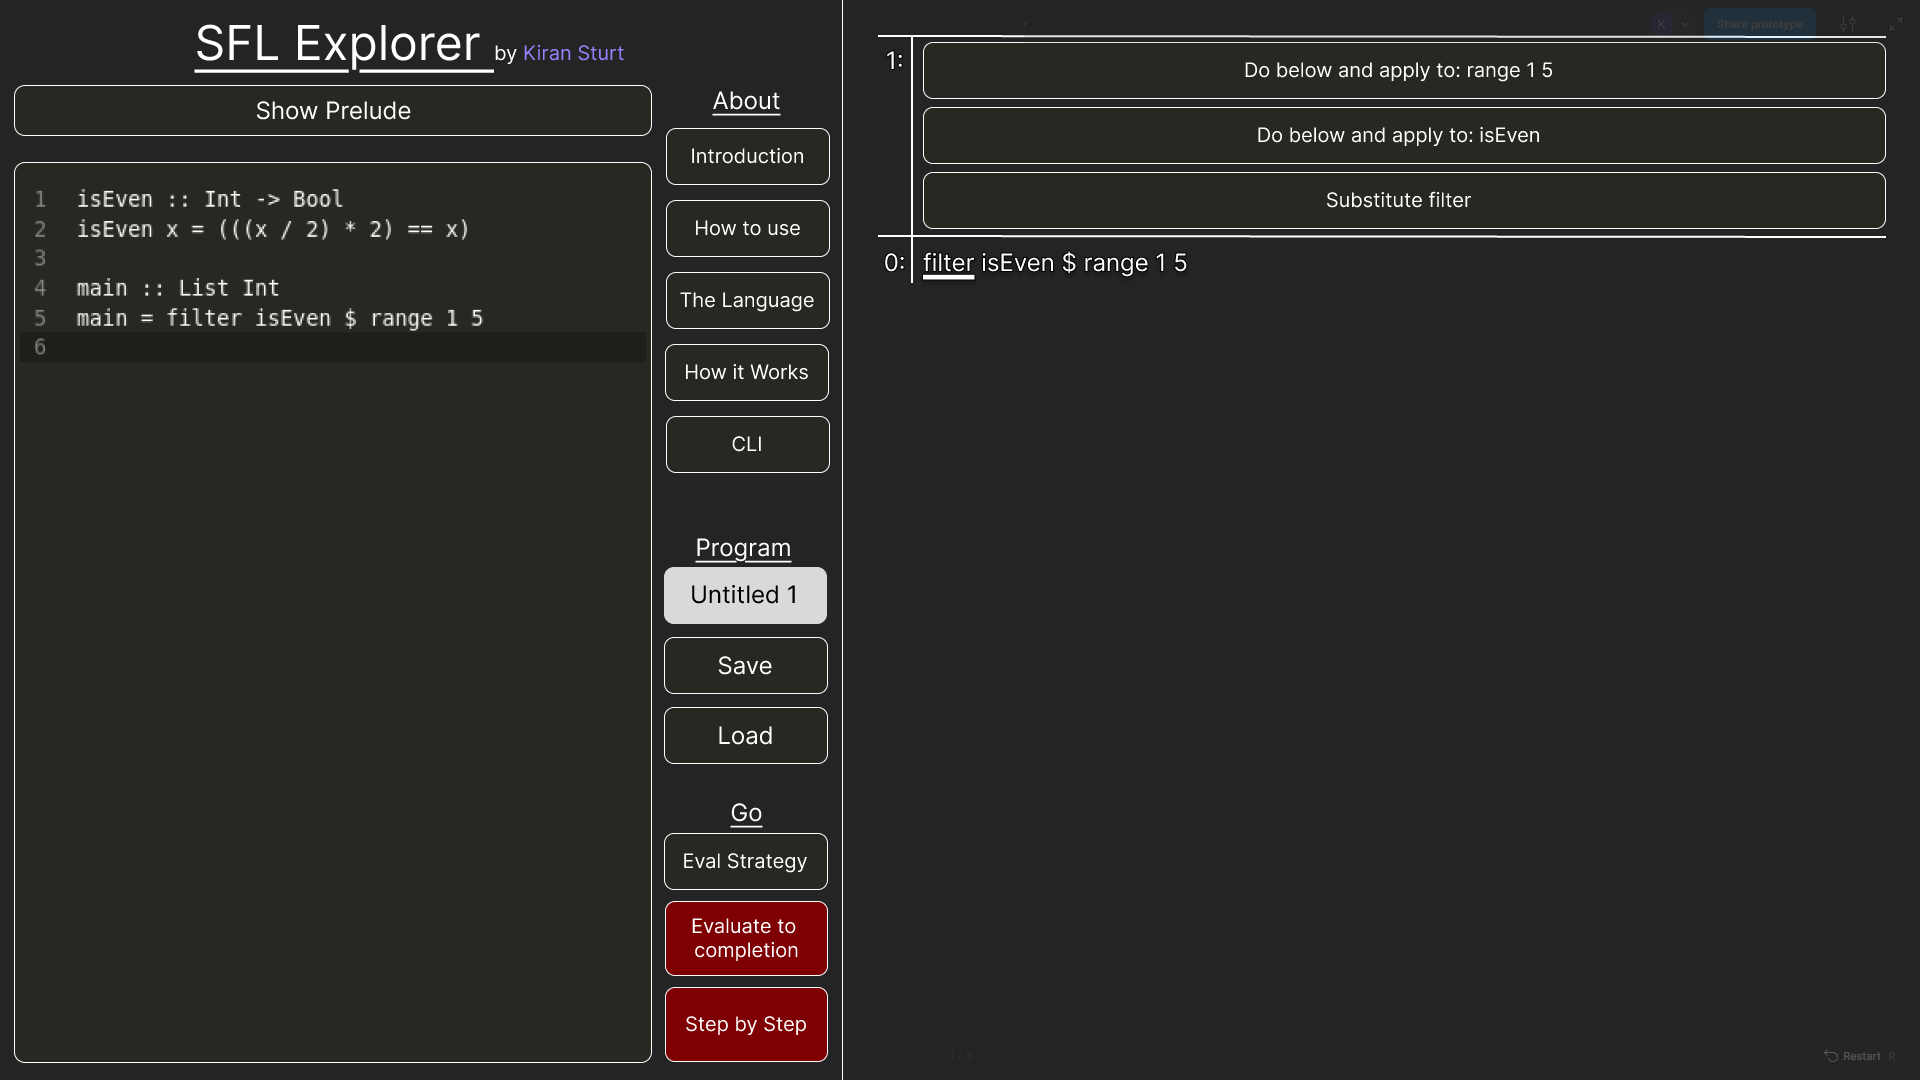
\includegraphics[width=1\linewidth]{images/figma_1.png} 
    \captionsetup{justification=centering}
    \caption{Screenshot 1 of the Figma design of the web UI.
    % \sam{formatting bug bear: put full stops at the end of captions}
    }
    \label{fig:screenshot_figma1}
\end{figure}

\begin{figure}[h]
    \centering
    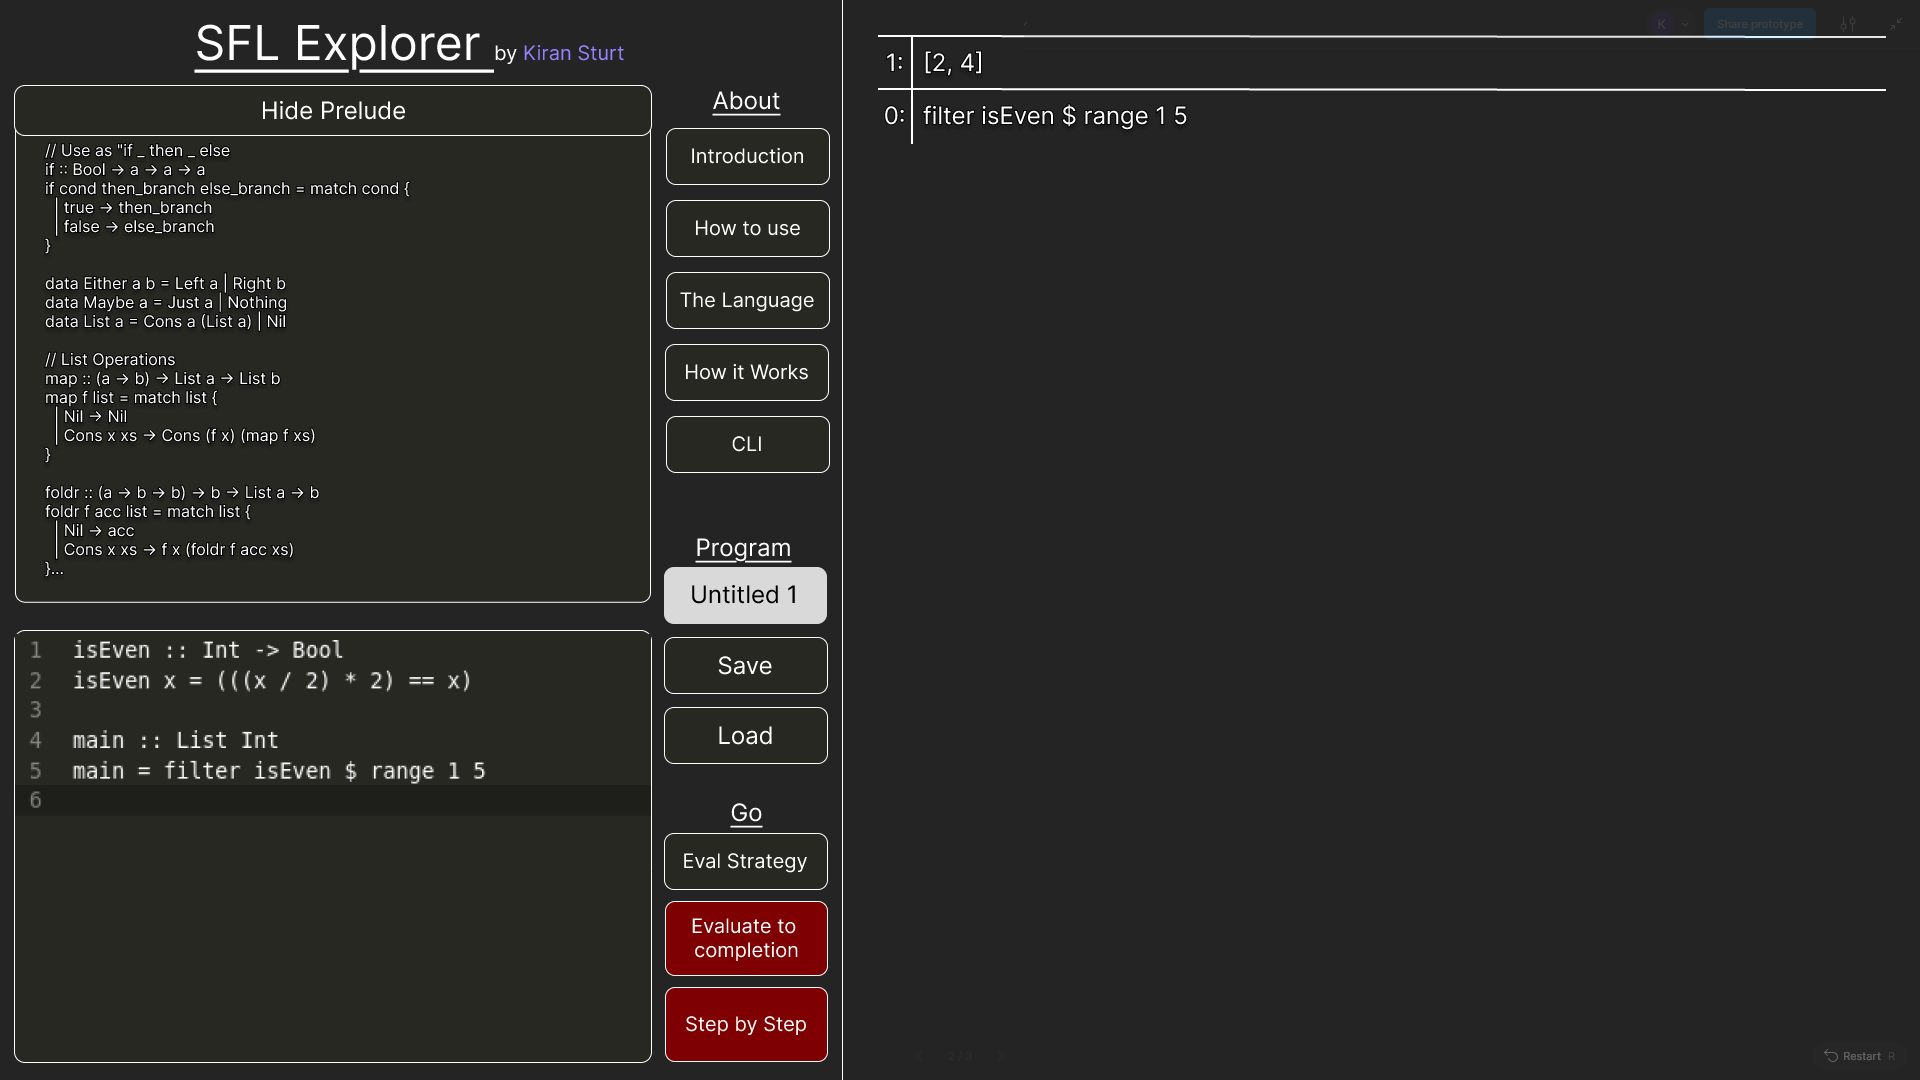
\includegraphics[width=1\linewidth]{images/figma_2.png}
    \captionsetup{justification=centering}
    \caption{Screenshot 2 of the Figma design of the web UI. This version shows the prelude dropdown extended. }
    \label{fig:screenshot_figma2}
\end{figure}

This design was meant to be a work in progress, but it looks quite similar to the final release of the product (Screenshots \ref{fig:screenshot_final_dark}, \ref{fig:screenshot_final_light}, \ref{fig:screenshot_final_dark_prelude_free} and \ref{fig:screenshot_final_light_prelude_free}). Before implementing this design, I discussed this design with the Advanced Focus Group (see \ref{ref:afg_figma}) and they were much more positive about this UI than the existing one.
% \todo{Discuss revert}\\
% \todo{Design principle: simplicity, speed, minimalism, feeling like vscode.}

\section{Implementation}

\subsection{Pairs}
% \todo{motivate pairs, Algebraic data types}
To support pairs, we must first add `Pair' as an option to our enum `\verb|ASTNodeType|' \ref{fig:ast_lst}. A `Pair' node has \verb|ASTNodeType| of `Pair', and two children.

\subsubsection{Parsing Pairs}
Parsing pairs is trivial:
\begin{itemize}
    \item Expect an open parenthesis \verb|(|.
    \item Parse an expression.
    \item Expect a comma.
    \item Parse a second expression.
    \item Expect a closing parenthesis \verb|)|.
\end{itemize}
\noindent We then produce a `\verb|Pair|' \ac{AST} node with two children: the two expressions.
\subsubsection{Updating the Redex Finding System With Pairs}
Pairs themselves can never be redexes, so getting a list of all redex-contraction pairs in a `Pair' is trivial: we concatenate the list of \verb|RCPairs| in the left and right expression.

\subsection{Pattern Matching}
We add `Match' as an option to our enum `\verb|ASTNodeType|' \ref{fig:ast_lst}. The first node represents the expression being matched over, then each case followed by its corresponding definition.
 
\subsubsection{Parsing Match Statements}
An example of using a match statement follows:
% \sam{here it feels like you are trying to mix up the way you introduce code so it is not always the same, but instead you have just ended up with a weird sounding sentence. It doesnt matter if introducing code uses the same phrasing, as long as it is clear.}
% \sam{more writing advice: only spend effort on nice writing for what is important. Introducing code not important, just do the basic thing. Biggest most complicated thing in your thesis is what deserves all your word choice and imagery. If you do this, it is also clear to the reader what is important: it is what you have spent your time on}
\begin{lstlisting}[language=SFL]
lengthIsAtLeast2 list = match list {
  | Cons x (Cons y xs) -> true
  | _ => false
}
\end{lstlisting}

The algorithm used for parsing match statements is:
\begin{enumerate}
    \item Consume the `match' keyword.
    \item Parse the expression matched over.
    \item Consume an open brace.
    \item While the next token isn't a close brace: \begin{enumerate}
        \item Consume bar `|'.
        \item Parse a pattern (\ref{impl:parsing_patterns}).
        \item Consume a right arrow.
        \item Parse an expression.
    \end{enumerate}
    \item Consume a close brace.
\end{enumerate}
This creates a `match' node, where the \verb|children| vector is set appropriately with the pattern and expressions.

\paragraph{Patterns}
\label{impl:parsing_patterns}
A pattern must not contain anything that can be reduced. It would be nonsensical to have a situation where we had a pattern not in normal form such as \verb|1 + 1| and the expression to be matched was \verb|2|. 

To parse a pattern, we may use the same techniques as parsing an expression, with a few differences:
\begin{itemize}
    \item Disallowing abstractions and match statements
    \item Identifiers must be either
    \begin{itemize}
        \item Unbound lowercase variables
        \item Underscore (\verb|_|) representing a wildcard pattern
        \item A bound uppercase variable (a constructor)
    \end{itemize}
\end{itemize}

\subsubsection{Updating the Redex Finding System With Pattern Matching}
As discussed in the design (\ref{c2_design_match}), patterns are checked in order from first to last. Not only do we need to check that it does not currently match before moving on to checking the next pattern, we must check that it \textit{can not} match the expression i.e. we must refute the pattern. In the below example, \sflinline{repeat 1} must be evaluated enough to know whether it matches the first pattern before we move on to matching the second. 

\begin{lstlisting}[language=SFL]
// Repeat is in the prelude, but it is shown here for convenience
repeat :: a -> List a
repeat n = Cons n (repeat n)

main :: Bool
main = match repeat 1 {
    | Cons _ (Cons _ _) -> true
    | _ -> false
}
\end{lstlisting}

When matching an expression against a pattern, we have three possible results:

\begin{itemize}
    \item Success: Matching was successful, and we have a list of what to bind.
    \item Refute: We can not match this pattern, and evaluating the expression further would definitely not result in being able to match.
    \item Unknown: It does not match, but we cannot refute.
\end{itemize}
\noindent The algorithm for finding the next evaluation step for a match expression is to sequentially attempt to match each pattern. If the result of matching an expression is a refutation, we check the next one. If the result is not yet known, we do not look at any further patterns, and we evaluate the expression further instead. 

Below is a short summary of how pattern matching is done for different structures. This summary does not show all cases, but instead aims to give a general idea about how the algorithm works. The full algorithm is listed in appendix~\ref{appx:pattern_match}. To match an expression $E$ against a pattern $P$ and get all variables that the pattern would bind, we proceed case wise on the structure of $P$. 
\begin{itemize}
    \item An Identifier \ref{fig:pattern_list_id}. 
    \begin{itemize}
        \item If the identifier is a lowercase variable, we succeed matching and returning the binding.
        \item If it is an underscore, matching succeeds, but we do not bind anything. 
        \item If it is an uppercase identifier (and therefore a constructor), we attempt to refute the pattern by showing that our expression will never evaluate to this constructor. Otherwise, our result is `unknown'.
    \end{itemize}

    % \item A pair: \ref{fig:pattern_list_pair}. We proceed case wise on the structure of $E$:
    % \begin{itemize}
    %     \item Another pair: we attempt to match the left and right of both pairs. If either Refutes then Refute, and if either is Unknown then return Unknown.
    %     \item Literal, Abstraction or Uppercase Identifier: Refute.
    %     \item Lowercase Identifier: Unknown, as it may stand for an expression that does evaluate to a pair
    % \end{itemize}
    
    \item An application: \ref{fig:pattern_list_app}. We proceed case wise on the structure of $E$:
    \begin{itemize}
        \item Literal, Pair, Abstraction or Uppercase Identifier: Refute as these will not evaluate further.
        \item Another application: Match the functions and match the arguments. If either Refutes then Refute, and if either is Unknown then return Unknown. Otherwise, Succeed, and concatenate the two lists of bindings
    \end{itemize} 

    \item A literal: If the expression is a literal, we perform a string match to figure out if this is a similarity or a difference. 
\end{itemize}

\noindent The algorithm for matching an expression against a single pattern, and getting either `Success, Refute, or Unknown' is listed in pseudocode~\ref{fig:pattern_list_top_level}. The algorithm for getting a redex-contraction pair from a match statement is also listed \ref{fig:all_pattern_list_iterate}, but to summarise:

\begin{itemize} 
    \item If we succeed in pattern matching, the result should be the appropriate case with all the bindings substituted. 
    \item If we have not yet succeeded or refuted all patterns, we look for a redex-contraction pair in the expression being matched. 
    \item If we have refuted all patterns, we fail to get a redex-contraction pair 
\end{itemize}


\subsection{Types}
Rust allows us to represent our types (see \ref{fig:tc_types} for the definition of the type system) quite easily using Enums. Rust's Enums are an example of an algebraic data type themselves, and are very useful for defining our own algebraic data type system. See \ref{fig:type_lst} for the listing. 
The type `$\alltype{a\;b} (a \arr b) \arr IntAlias \arr List\,a \arr List\,b$' where $IntAlias$ is defined by `\sflinline{type IntAlias = Int}' would be represented in this implementation (ignoring the `\verb|Box|'s) as:    
\begin{lstlisting}[language=Rust_boxed]
Forall("a", 
  Forall("b", 
    Function(
      Function(
        TypeVariable("a"), 
        TypeVariable("b")
      ),
      Alias("IntAlias", Int)
      Function(
        Union("List", [TypeVariable("a")]), 
        Union("List", [TypeVariable("b")])
      )
    )
  )
)
\end{lstlisting}


\begin{figure}[ht]
    % \centering
    % \begin{tabular}{c}
    % \hline
    \begin{lstlisting}[language=Rust_boxed]
pub enum PrimitiveType {
    Int,
    Bool,
}

pub enum Type {
    Unit,
    Primitive(PrimitiveType),
    Function(Box<Type>, Box<Type>),
    TypeVariable(String),
    Forall(String, Box<Type>),
    Product(Box<Type>, Box<Type>),
    Union(String, Vec<Type>),

    Alias(String, Box<Type>),
    Existential(usize),
}
\end{lstlisting}
    % \\\hline
    % \end{tabular}
    \caption{The Rust code listing for the definition of types. `Existential' and `Alias' are separated as they are more of an implementation detail than a part of the type system}
    \label{fig:type_lst}
\end{figure}

% We must use \verb|Box<Type>|, which represents a pointer to a heap allocated object, otherwise it would be impossible to calculate the size of \verb|Type|, as it could be infinitely large with it containing another \verb|Type| recursively. \verb|Box<Type>| however has known size: the size of a pointer in the target architecture. 

\noindent Aliases are defined here with their name, and the type they are an alias for. Aliases could simply be implemented by replacing all occurrences of the alias with the type, but defining them here allows us to use their names to generate type errors making them easier to understand. We also define existential as an implementation detail for the typechecker. 

\subsubsection{Methods on Types}
Below are a selection of the more important or interesting methods implemented on Types.

\paragraph{Substitution of type variables} If we have a function of type $\alltype{a\;b} a \arr b \arr a$, and we apply it to a term with type $Int$, to figure out the type of the application we would substitute all of the $a$s in the type with $Int$, and remove the $\forall a$, leaving us with $\alltype{b} Int \arr b \arr Int$. 

%We  if given the type expression \(T \; U\) where \(T\) and \(U\) are types, and we know that one of the constructors of \(T\) is of generic type \(\forall a.a \rightarrow T \; a\), the type of the constructor for this type should be \(U \rightarrow T \; U\). We have `instantiated' the type variable \(a\) to be \(U\) by substituting \(a\) with \(U\) throughout the expression, and removing the \(\forall a\). This is required for the type checker. 

\paragraph{To String} We will frequently wish to display types as strings for debugging purposes. This is done recursively

\subsection{Parsing Types}
In the proof of concept system, the parser simply returns an AST. In order to parse a program with user defined types, type assignments, and pattern matching, the parser should return:
\begin{itemize}
    \item The AST.
    \item The `Label Table': The types of all labels defined, including both those defined explicitly (assignments) or implicitly (constructors). This is implemented as `\verb|HashMap<String, Type>|'. 
    \item The `Type Table': All type constructors and type aliases defined, stored as a `\verb|HashMap<String, Type>|'. Aliases are stored with their name, and the type they are an alias for. Type constructors defined by data declarations are stored with all of their variables in nested foralls. For instance, parsing the data declaration (ignoring the data constructors), `\sflinline{data Either arg1 arg2 = ...}' would add to our type table the type the entry: $Either : \alltype{a\;b} Either\;a\;b$
\end{itemize}
For instance, from the program:
\begin{lstlisting}[language=SFL_noprelude]
data List a = Cons a (List a) | Nil
type IntAlias = Int
double :: IntAlias -> IntAlias
double x = x + x	
\end{lstlisting}
We should extract the following data:
\begin{itemize}
    \item The AST: 
    \begin{lstlisting}[]
Module:
  Assignent
    Identifier: double
    Abstraction
      Identifer: x
      App
        App
          Identifier: +
          Identifier: x
        Literal: 2
    \end{lstlisting}
    \item All the known type assignments (excluding inbuilts).
        \begin{itemize}
            \item Cons: \(\forall a. a \Rightarrow List\;a\Rightarrow List\;a\).
            \item Nil: \(\forall a. List\;a\).
            \item double: \(IntAlias \arr IntAlias\).
        \end{itemize}
    \item The names of all known types (excluding inbuilts) 
        \begin{itemize}
            \item List: a type constructor with arity 1.
            \item IntAlias: a type alias pointing to Int.
        \end{itemize}
\end{itemize}

\subsubsection{Parsing Type Expressions}
The parser needs to be able to parse type assignments (\verb|x :: Int|) and type declarations (\sflinline{type}, or \sflinline{data}). Parsing both of these things require the ability to parse type expressions, such as `\sflinline{Int}' and `\sflinline{a -> a}'. Type expressions can be parsed using recursive descent parsing. Our connective for our parsing is arrow `\verb|->|', and our primaries are anything that does not contain arrow (except in parenthesized expressions). The structure of the type expression parser is similar to that of the expression parser. We first parse a primary, and then we terminate or parse our connective.

However, if we are parsing a type expression for an assignment, we will need to prepend our the type generated by parsing a type expression with existential quantifiers for each of the type variables used. For instance, if we have an assignment `const' with a type assignment \sflinline{const :: a -> b -> a}, this is interpreted as ${\alltype{a\;b} a \arr List\;b \arr List\;a}$.

\paragraph{Parsing Type Expression Primaries}
To parse a type expression primary, we consume a token $T$ and progress differently based on what this token was:
\begin{itemize}
    \item If $T$ is an open bracket, we parse a type expression, then expect a closing bracket. 
    \item If $T$ is an uppercase identifier, it must be a type constructor. We check the current state of the \verb|type_table| to see if it exists. If it does, we return it by converting it into a `union' type with the correct number of arguments. 
\end{itemize}

% There are 

% \todo{Convert to prose}
% \begin{figure}
% \begin{lstlisting}[language=SFL]
% fn parse_type_expression_primary(bound_type_variables, type_table) {
%     next_token = consume()
%     match (next_token) {
%         case lowercase_id {
%             name = next_token.value
%             if bound_type_variables exists {
%                 if !bound_type_variables.contains(name) {Error}
%             }
%             return TypeVariable(name)
%         }
%         case uppercase_id {
%             name = next_token.value
%             if type_table.contains(name) {
%                 return type_table.get(name)
%             } else {Error}
%         }
%         case left_paren {
%             return parse_type_expression(bound_type_variables, type_table)
%         }
%         otherwise Error
%     }
% }
% \end{lstlisting}
% \caption{The algorithm for parsing }
% \end{figure}

\subsubsection{Parsing Type Alias Definitions} 
We may wish to add another name that a type can be known by. For instance, we may wish to define `\verb|String|' as a list of characters, so that we may reference it easier. A type alias declaration consists of:
\begin{itemize}
    \item The `\verb|type|' keyword.
    \item The name of the alias.
    \item The assignment operator ($=$).
    \item The type expression.
\end{itemize}
The function that produces type aliases returns a `\verb|Type::Alias(String, Box<Type>)|'. The reason we do not want to simply rename all references to the alias name to the type in question is that this would make type errors more obscure, and harder for users to understand the error with reference to the original program.

\subsubsection{Parsing Data Declaration} 
We want to be able to define and parse \verb|data| declarations~\ref{c2:design_data_types}. A \verb|data| deceleration consists of: 
\begin{itemize}
    \item The \sflinline{data} keyword.
    \item The name of the type (uppercase ID) .
    \item A list of type variables. We continually expect a lowercase identifier token until we reach the assignment operator `\verb|=|'. The lowercase identifiers (type variables) declared are passed to the functions that parse constructors so that we can enforce that all of the type variables used in the constructor parsing are `in scope'. We also do this to make sure that the variables are correct. 
    \item The assignment operator (=).
    \item A set of constructors separated by \(\mid\). Constructor definitions consist of the following. 
        \begin{itemize}
            \item The name of the constructor
            \item Zero or more type expressions, representing what types the constructor can be applied to. These type expressions must only contain type variables in the set before the assignment operator, but can be any other concrete type expression.  
        \end{itemize}
\end{itemize}

\noindent An example definition is: `\sflinline{data Either a b = Left a | Right b}'. The information that should be extracted from here is:
\begin{itemize}
    \item `\verb|Either|' is a type constructor with a kind of \(*\rightarrow* \rightarrow *\). We store this as $\alltype{a\;b} Either\;a\;b$.
    \item The constructors and their types are:
    \begin{itemize}
        \item `\verb|Left|': \(\forall a\;b.a\rightarrow Either\;a\;b\)
        \item `\verb|Nil|': \(\forall a\;b.b\rightarrow Either\;a\;b\)
    \end{itemize}
\end{itemize}

\noindent 
\paragraph{Parsing Data Constructors}

Parsing constructors is not complex, as we have already implemented the mechanism for parsing type expressions. We simply keep parsing expressions until either the constructor separator ($\mid$) or a newline is reached. When parsing the type expression, we expect only valid concrete types in the Type Table, or valid in scope type variables from the type constructor definition. We then produce a type from the types of the arguments in order, with all of the type variables declared lifted to the start of the type into a series of nested `\verb|Type::Forall|'s. 
\begin{lstlisting}[language=SFL]
data EGType a b c = EGCnstr1 a Int b | EGCnstr2 Bool c | EGCnstr3 b c a
\end{lstlisting}
\noindent For instance, the above data declaration creates constructors:
\begin{itemize}
    \item \verb|EGCnstr1|: \(\alltype{a\,b\,c} a \arr Int \arr b \arr EGType\;a\;b\;c\).
    \item \verb|EGCnstr2|: \(\alltype{a\,b\,c} Bool \arr c \arr EGType\;a\;b\;c\).
    \item \verb|EGCnstr3|: \(\alltype{a\,b\,c} b \arr c \arr a \arr EGType\;a\;b\;c\).
\end{itemize}



% so the constructor definition `\verb|ConstructorName a b|', results in the type `\(a \rightarrow b \rightarrow  TypeName\)'

\newpage
\subsection{The Type Checker}
\begin{figure*}[t]
    \begin{minipage}{1\textwidth}
    \judgbox{\chkjudg{\Gamma}{e}{A}{\Delta}}%
    {Under input context $\Gamma$, $e$ checks against input type $A$, 
    with output context $\Delta$} \\[1ex]
 \judgbox{\synjudg{\Gamma}{e}{A}{\Delta}}%
    {Under input context $\Gamma$, $e$ synthesizes output type $A$,
      with output context $\Delta$} \\[0.5ex]
 \judgbox{\appjudg{\Gamma}{e}{A}{C}{\Delta}}%
    {Under input context $\Gamma$, applying a function of type $A$ to $e$ synthesizes type $C$, \\ with output context $\Delta$} \\
    \end{minipage}
    \noindent\rule{\textwidth}{0.4pt}
    \caption{From~\cite{completebidir}: Checking and Synthesis judgements the typechecking algorithm attempts to derive. }
    \label{fig:bidir_judgement_types}
\end{figure*}

The type checker uses an algorithm which is a modified version of the algorithm proposed by Dunfield and Krishnaswami \cite{completebidir}. 
\begin{quote}
`Bidirectional typechecking, in which terms either synthesize a type or are checked against a known type, has become popular for its scalability \ldots\ its error reporting, and its relative ease of implementation' \cite{completebidir}
\end{quote}
\noindent It was the `relative ease of implementation' that attracted me to bidirectional type checking. I modified their algorithm to add my extra types (the inbuilt types $Int$, $Bool$, as well as the \Uniontype\ and \Producttype\ types) and my extra expression syntax structures (literals, match, pairs). This does not include assignment and modules as these are not part of expression syntax. 

\begin{figure}[h]
  \centering
  \begin{minipage}{\textwidth}
  \[
      \begin{array}{llcl}
      % \\[4pt]
      \text{Types} & A, B, C & \bnfas &
            \Inttype \bnfalt \Booltype \bnfalt \alpha \bnfalt \ahat \bnfalt 
            % \\[1pt] &&&\!\!\!\;\;\;
            \alltype{\alpha}{A} \bnfalt A \arr B \bnfalt
            % \\[1pt] &&&\!\!\!\;\; \TypeAlias{A}{B} \bnfalt  
            % \\[1pt] &&&\!\!\!\;\;
            (A, B) \bnfalt
            % \\[1pt] &&&\!\!\!\;\;
            \Unionname[A_1, \dots, A_n]
      \\[2pt]
      \text{Monotypes} & \tau,\sigma & \bnfas &
            \Inttype \bnfalt \Booltype \bnfalt \alpha \bnfalt \ahat \bnfalt 
            % \\[1pt] &&&\!\!\!\;\;
            \tau \arr \sigma \bnfalt (\tau, \sigma) \bnfalt \Unionname[\tau_1, \dots, \tau_n]
            % (A, B) \bnfalt \TypeAlias{A}{B}
        \\[2pt]
      \text{Contexts} & \Gamma, \Delta, \Theta & \bnfas &
                  \cdot
                  \bnfalt \Gamma, \alpha 
                  \bnfalt \Gamma, x:A
                  % \\[1pt] &&&\!\!\!\;\;
                  \bnfalt \Gamma, \ahat
                  \bnfalt \Gamma, \hypeq{\ahat}{\tau}
                  % \\[1pt] &&&\!\!\!\;\;
                  \bnfalt \Gamma, \MonnierComma{\ahat}
      % \\[2pt] % No need as I am not proving completeness
      % \text{Complete Contexts}     & \Omega & \bnfas &
      %             \cdot
      %             \bnfalt    \Omega, \alpha
      %             \bnfalt    \Omega, x:A
      %             \\[1pt] &&&\!\!\!
      %             \bnfalt    \Omega, \hypeq{\ahat}{\tau} 
      %             \bnfalt    \Omega, \MonnierComma{\ahat}
      \end{array}
  \]
  
  \captionsetup{justification=centering}\caption{Syntax of types, monotypes, and contexts as seen by the typechecker. The definition of types differ slightly from the definition offered in figure \ref{fig:sfl_types_no_exst}, as we include existential type variables ($\ahat$) that can not actually be created by users. They are an implementation detail required for the type checking algorithm}
  \FLabel{fig:tc_types}

  
  \end{minipage}
  \hfill
  \begin{minipage}{\textwidth}
    \centering
      \[
  \begin{array}[t]{l@{~}c@{~}ll}
      %
      [\Gamma]\Inttype  & = & \Inttype &\\{}

      [\Gamma]\Booltype & = & \Booltype &\\{}

      [\Gamma]\alpha    & = & \alpha &\\{}
      % [\Gamma]\unitty   & = &   \unitty &
      % \\[1pt]
      \big[\Gamma[\hypeq{\ahat}{\tau}]\big] \ahat
               & = &   \big[\Gamma[\hypeq{\ahat}{\tau}]\big]\tau &
      \\[2pt]
      \big[\Gamma[\ahat]\big]\ahat   & = &   \ahat &
      \\[2pt]
      [\Gamma](A \arr B)   & = &
          ([\Gamma]A) \arr ([\Gamma]B) &
      \\{}
      [\Gamma](\alltype{\alpha} A)
         & = & 
         \alltype{\alpha} [\Gamma]A &
      \\[2pt]
      [\Gamma](A, B) 
         & = &
         ([\Gamma]A, [\Gamma]B)
      \\[2pt]
      [\Gamma]\Unionname[A_1,\dots, A_n]
         & = &
         \Unionname[[\Gamma]A_1,\dots, [\Gamma]A_n]
  \end{array}
  \]
  \captionsetup{justification=centering}\caption{Applying a context, as a substitution, to a type}
  \FLabel{fig:ctx_subst}
  \end{minipage}
\end{figure}


% The full typechecking algorithm is listed in figures \ref{fig:alg-subtyping}, \ref{fig:instantiation}, \ref{fig:alg-typing}. Below I will describe the typechecking algorithm, focusing on my additions/changes. This will then be followed by two example derivations. Appendix \ref{appx:example_derive} shows some example derivations using this algorithm including some of my rules. 

\noindent The typechecking algorithm (Figure~\ref{fig:alg-typing}) is presented as a series of \textit{inference rules}, which describe how to derive conclusions (written below the horizontal line) from a set of premises (written above it). 
These rules allow us to construct \textit{derivation trees} by starting from the conclusion we wish to prove and recursively deriving each premise, continuing until we reach axioms - rules with no premises.
The conclusions derived in this way are called \textit{typing judgements}. A typical typing judgement takes the form $\judge{\Gamma}{x}{A}$, meaning `under context $\Gamma$, it is derivable that $x$ has type $A$'. However, in our bidirectional type system, we have three different types of typing judgements we attempt to derive~(see~\ref{fig:bidir_judgement_types}), and in the process of deriving these judgements we also update our context with additional information gleaned during the derivation process. 
\begin{figure}[!h]
    \begin{mathpar}
    \Infer{\MyTCRule{\Paircheckrulename}}
        {\chkjudg{\Gamma}{e_1}{A}{\Theta} \\ \chkjudg{\Theta}{e_2}{B}{\Delta}}
        {\chkjudg{\Gamma}{(e_1, e_2)}{(A, B)}{\Delta}}
    \end{mathpar}
    \caption{One of the inferrence rules in the algorithm, listed here as an example. }
    \label{fig:eg_infer_rule}
\end{figure}

\pagebreak
\paragraph{\textbf{Pair}$\chk$, an Example Inference Rule} Figure~\ref{fig:eg_infer_rule} shows an example inference rule which I added to the algorithm, \MyTCRule{\Paircheckrulename}. It allows us to derive that a pair $(e_1, e_2)$ checks against type $(A, B)$ under context $\Gamma$ with output context $\Delta$ (${\chkjudg{\Gamma}{(e_1, e_2)}{(A, B)}{\Delta}}$) if $e_1$ checks against $A$ under context $\Gamma$ with output context $\Theta$ (${\chkjudg{\Gamma}{e_1}{A}{\Theta}}$) and if $e_2$ checks against $B$ under context $\Theta$ with output context $\Delta$ (${\chkjudg{\Theta}{e_2}{B}{\Delta}}$).

\paragraph{Well Formed Types} 
\label{c2:types_well_formed}
Figure~\ref{fig:algorithmic-wf} shows the algorithm for deriving that under context $\Gamma$, type $A$ is well-formed. It just checks that our context $\Gamma$ \textit{knows about} and existential type variables in $A$. For instance, under context $\Gamma = (\ahat, \bhat = Int)$, type $\ahat \arr \bhat$ is well-formed, but $\ahat \arr \chat$ is not. 

\begin{figure}
\judgbox{\judgetp{\Gamma}{A}}{Under context $\Gamma$, type $A$ is well-formed}
\begin{mathpar}
    \Infer{\UvarWF}
          { }
          { \judgetp{\Gamma[\alpha]}{\alpha} }
    \and
    \Infer{\UnitWF}
          { }
          { \judgetp{\Gamma}{\unitty} }
    \and
    \Infer{\ArrowWF}
          { \judgetp{\Gamma}{A} \\ \judgetp{\Gamma}{B} }
          { \judgetp{\Gamma}{A \arr B} }
    \and
    \Infer{\ForallWF}
          { \judgetp{\Gamma, \alpha}{A} }
          { \judgetp{\Gamma}{\alltype{\alpha}{A}} }
    % \vspace{-1.3ex}
    % \\
    \Infer{\EvarWF}
          { }
          { \judgetp{\Gamma[\ahat]}{\ahat} }
     ~~~~
    \Infer{\SolvedEvarWF}
          { }
          { \judgetp{\Gamma[\hypeq{\ahat}{\tau}]}{\ahat} }
\end{mathpar}
\caption{From~\cite{completebidir}: Well-formedness of types and contexts in the algorithmic system. }
\FLabel{fig:algorithmic-wf}
\end{figure}

\paragraph{Hole notation}
Below is a paragraph from the original paper \cite{completebidir} explaining `hole notation' in contexts, which is used throughout the algorithm descriptions in \ref{fig:alg-typing}, \ref{fig:alg-subtyping} and \ref{fig:instantiation}. 
\begin{quote}
`Since we will manipulate contexts not only by appending declarations \dots but by inserting and replacing declarations in the middle, a notation for contexts with a hole is useful:
\vspace{-4pt}
\begin{displ}
  `$\Gamma = \Gamma_0[\Theta]$~~~means $\Gamma$ has the form $(\Gamma_L, \Theta, \Gamma_R)$
\end{displ}
For example, if $\Gamma = \Gamma_0[\bhat] = (\ahat, \bhat, x : \bhat)$,
then $\Gamma_0[\hypeq{\bhat}{\ahat}] = (\ahat, \hypeq{\bhat}{\ahat}, x : \bhat)$
% \sam{what is $\hypeq{\bhat}{\ahat}$ why are there two $\bhat$}
\newline\dots\newline
% \sam{...?}
% \sam{this is the most complex thing so far, here is where you need to spend your time, and start with an example}
% \sam{yes you are building on prev work, so your extensions are of most interest, but i cant appreciate them if i dont understand the base algo, also you must demo that you know the base algo}
Occasionally, we also need contexts with \emph{two} ordered holes:
\begin{displ}
  $\Gamma = \Gamma_0[\Theta_1][\Theta_2]$
  ~~~means
  $\Gamma$ has the form $(\Gamma_L, \Theta_1, \Gamma_M, \Theta_2, \Gamma_R)$' \cite{completebidir}
\end{displ}
\end{quote}

% \sam{please run a small example inline here}
% \sam{you cannot rely on readers looking at your appendix}
% \sam{now i have read the appendix, It is excellent!!! just move that. Its so much clearer and its not dry cos we gave a goal and it nicely guides me through}

\subsubsection{Algorithmic Type Checking and Synthesis}
Figure~\ref{fig:alg-typing} shows the algorithm for checking and synthesizing the types of various expression structures. The rules I added are: 
%\sam{questions the reader might have: but how is this an algo? they are sequences of steps? What is all this notation? I've never seen the backwards turnstyle before or the backward implication. This should be walked thorugh in prose, you should not expect me to spend ages looking at the figure figuring it out. You are the writer, guide me}
%\sam{say in the prose that they are highlighted. I think the way you use captions is weird. It reads as if your expectation upon someone reading "figure bla" is that they immediately read the caption of figure  bla, but i dont. I stick with the prose hoping to be guided through my viewing of the figure, especially such a complex one.}
\begin{itemize}
    \item Checking and synthesizing rules for values of type $Int$ and $Bool$: An integer literal synthesizes the type $Int$, and checks against the type $Int$ etc. 
    %\sam{there is a way to reference rules, which might be nice here}
    \item Checking and synthesis rules for pairs
    \begin{itemize}
        \item A pair $(e_1, e_2)$ checks against type $(A, B)$ if $e_1$ checks against $A$ and $e_2$ checks against $B$ (see \ref{fig:eg_infer_rule}). 
        \item If $e_1$ synthesizes type $A$ and $e_2$ synthesizes type $B$ then $(e_1, e_2)$ synthesizes $(A, B)$
    \end{itemize}
    \item The rule for synthesizing the type of a match expression. We synthesize the type of the expression being matched to a type $A$ (\synjudg{\Gamma}{e}{A}{\Delta}). We then check all the types of the patterns against type $A$. To get the output type, we add an existential type variable $\ahat$ to our context, and then check the type of all the output expressions against the type $\ahat$. We synthesize the type $\ahat$. The context is passed through all of these operations, and the final context contains all of the things `learned' from typechecking the match expression. 
    % \sam{this is better, but match each sentence to the symbols you are describing, I've inlined an example}
\end{itemize}

\noindent Note that the checking rules $\MyTCRule{\Intcheckrulename}$, $\MyTCRule{\Boolcheckrulename}$, $\MyTCRule{\Paircheckrulename}$ are not actually necessary, as they could be caught by the $\Sub$ rule. They are included as they remove the unnecessary steps that using the $\Sub$ rule in this manner creates, speeding up/simplifying the algorithm. For instance, figure~\ref{int_reduced_deriv_steps} shows how we can derive \chkjudg{\Gamma}{Int Literal}{\Inttype}{\Gamma} in two different ways.

\begin{figure}
    \begin{mathpar}
    \Infer{\MyTCRule{\Intcheckrulename}}
        { }
        {\chkjudg{\Gamma}{Int Literal}{\Inttype}{\Gamma}}
    \and 
    \Infer{\Sub}
    {\Infer{\MyTCRule{\Intsynthrulename}}
    { }
    {\synjudg{\Gamma}{Int Literal}{\Inttype}{\Gamma}}
      \\
    \Infer{\MyTCRule{\Intsubrulename}}
        { }
        {\subjudg{\Gamma}{\Inttype}{\Inttype}{\Gamma}}
    }
    {\chkjudg{\Gamma}{Int Literal}{\Inttype}{\Gamma} }
    
    \end{mathpar}
    \caption{Two ways of deriving \chkjudg{\Gamma}{Int Literal}{\Inttype}{\Gamma}, to show having both synthesis and checking rules, rather than just synthesis, can reduce the number of derivation steps. }
    \label{int_reduced_deriv_steps}
\end{figure}

\noindent If we are using this algorithm to synthesize a type, we may end up with a type containing existential type variables. At the end of inference, if an existential type variable has no constraints and is not free in the environment, we may generalize it to a universal quantifier (i.e., replace it with a $\forall$).

\subsubsection{Algorithmic Subtyping}
\begin{quotation}
\noindent `We say $S$ is a subtype of $T$, written as $S \subtype T$, to mean that any term of type $S$ can safely be used in a context where a term of type $T$ is expected'~\cite{pierce2002types}.
\end{quotation}
Figure \ref{fig:alg-subtyping} shows the inference rules used to construct a derivation that a type is a subtype of another type in \ac{SFL}. 
% For instance, our typechecking rule $\Sub$ synthesizes the type, and the uses the algorithmic subtyping rules to check that the synthesized type is a subtype of the expected type. 
I have added the following rules:
\begin{itemize}
    \item $Int \subtype Int$ and $Bool \subtype Bool$ trivially. 
    \item $(A_1, B_1) \subtype (A_2, B_2)$ if $A_1 \subtype A_2$ and $B_1 \subtype B_2$.
    \item The union with name $N_1$ and arguments $A_1 \dots A_n$ is a subtype of a union with name $N_2$ and arguments $B_1 \dots B_n$, if the names are the same, as the names uniquely identify these types, as well as all the constituent types being subtypes of each other in order. The context is passed through all of these operations, and the final context contains all of the things `learned' from typechecking the match expression.
\end{itemize}

\subsubsection{Context Instantiation} 
Figure \ref{fig:instantiation} shows the special subtyping rules for existential type variables that also instantiates the variable within the context. The subtyping rule $\SubInstL$ allows us to derive that the existential type variable $\ahat$ is a subtype of the type $A$. It requires that we instantiate $\ahat$ to the value of $A$ in our context. $\SubInstR$ does the opposite. Both add to the context all the information we gain about $\ahat$ by saying that it is a subtype of $A$, or that $A$ is a subtype of it. 

For instance, the rule $\InstLArr$ instantiates $\ahat$ such that $\ahat \subtype A_1 \arr A_2$ by adding to our context $\ahat_1, \ahat_2$, and setting $\ahat = \ahat_1 \fto \ahat_2$ in the context. We then instantiate $\ahat_1 \instsymlop A_1$ and $\ahat_2 \instsymrop A_2$.

\subsubsection{Examples Derivations}
Below are two example derivations that cover most of the key aspects of the algorithm. The first example~\ref{tc_eg_list} aims to give a simpler demonstration and explaination of how the typechecking and synthesis inference rules work, and use some of my rules. The second~\ref{c2:types_demo_2} aims to show a more complex derivation heavily relying on the context instantiation rules. A supplamentory derivation is included in the appendices~(\ref{appx:example_derive}), which shows more of my rules in action. 

\paragraph{Typechecking an Expression Involving Lists}
\label{c2:types_demo_1}
In figure~\ref{tc_eg_list}, we attempt to use the algorithm to check the type of \lstinline[language=SFL]|Cons 1 Nil| against \lstinline[language=SFL]|List Int|. In this derivation, the definition of $List$ is only over $Int$s to avoid the complexities of polymorphism, which are better demonstrated by the next example~\ref{c2:types_demo_2}:
\begin{lstlisting}[language=SFL]
data List = Cons Int (List Int) | Nil
\end{lstlisting}
\noindent The reason the context is never changed is as we do not have any abstractions or foralls, so no variables or type variables are introduced. Type checking/synthesis is done recursively from bottom up, so read [1] upwards. 

\begin{figure}[t]

\begin{mathpar}
T_{Nil} = List\;Int\and
T_{Cons} = {Int \fto List\;Int \fto List\;Int}\\
\Gamma = T_{Cons}, T_{Nil}\and\Gamma = \Gamma_0 = \Gamma_1\\

\\

\Infer{\MyTCRule{\Unionsubrulename}[10]}
    {\Infer{\MyTCRule{\Intsubrulename}[11]}{ }
        {\subjudg{\Gamma_0}{Int}{Int}{\Gamma_1}}}
    {\subjudg{\Gamma_0}{List[Int]}{List[Int]}{\Gamma_{1}}}
\\

\Infer{\ArrApp[7]}
    {     \Infer{\Sub[8]}
          { 
          {
          \Infer{\Var[9]}
            {(Nil : T_{Nil}) \in \Gamma}
            {\synjudg{\Gamma}{Nil}{T_{Nil}}{\Gamma}}
          }
            \\
            \subjudg{\Gamma}{List[Int]}{List[Int]}{\Gamma}[10]
          }
          {\chkjudg{\Gamma}{Nil}{List\;Int}{\Gamma}}}
    {\appjudg{\Gamma}{Nil}{List\;Int \arr List\;Int}{List\;Int}{\Gamma}}

\\
\Infer{\!\ArrElim[3]}
{
{
\Infer{\Var[4]}
    {(Cons : T_{Cons}) \in \Gamma}
    {\synjudg{\Gamma}{Cons}{T_{Cons}}{\Gamma}}
}
\\
    {
    \Infer{\ArrApp[5]}
        {
        \Infer{\MyTCRule{\Intcheckrulename}[6]}
            { }
            {\chkjudg{\Gamma}{1}{Int}{\Gamma}}
        }
        {\appjudg{\Gamma}{1}{T_{Cons}}{List\;Int \arr List\;Int}{\Gamma}}
     % \Infer{\AllApp}
     %    {\appjudg{\Gamma_1,\ahat}{1}{(\ahat \fto List\; \ahat \fto List\;\ahat)}{C}{\Delta}}
     %    {\appjudg{\Gamma_1}{1}{\alltype{\alpha}{\alpha \fto List\; \alpha \fto List\;\alpha}}{C}{\Delta}}
    }
    }
    {\synjudg{\Gamma}{Cons\,1}{List\;Int \arr List\;Int}{\Gamma}}
\\

\Infer{\!\ArrElim[2]}
    {
    {
        {\synjudg{\Gamma}{Cons\,1}{List\;Int \arr List\;Int}{\Gamma}}[3]
    }
    \\
    \appjudg{\Gamma}{Nil}{List\;Int \arr List\;Int}{List\;Int}{\Gamma}[7]
    }
    {\synjudg{\Gamma}{Cons\,1\,Nil}{List\;Int}{\Gamma}}
\\

\Infer{\Sub[1]}
    {
        {\synjudg{\Gamma}{Cons\,1\,Nil}{List\;Int}{\Gamma}}[2]
        \\
        \subjudg{\Gamma}{List[Int]}{List[Int]}{\Gamma}[10]
    }
    {\chkjudg{\Gamma}{Cons\;1\;Nil}{List\;Int}{\Gamma}}
\end{mathpar}
\caption{An example derivation showing typechecking of $Cons\;1\;Nil$ against $List\;Int$}
\label{tc_eg_list}
\end{figure}

\begin{enumerate}
    \item To check $Cons\;1\;Nil$ against $List\;Int$ [2], we first synthesize the expression type, and check the synthesized type is as subtype of $List\;Int$ [10].
    \item To synthesize the type of the expression $Cons\;1\;Nil$ (implicitly $(Cons\;1)\;Nil$) we synthesize the type of the left-hand side of the application $Cons\;1$ to be $List\;Int\arr List\;Int$ [3] and then we synthesize the type of $Nil$ under the application of that type [7], which gives us $List\;Int$.
    \item To synthesize the type of $Cons\;1$, we synthesize the type of the left-hand side of the application $Cons$ to be $T_{Cons}: Int\arr List\;Int\arr List\;Int$ [4], and then synthesize the type of $1$ under the application of that type, which gives us $List\;Int\arr List\;Int$ [5].
    \item We synthesize the type of $Cons$ to be $T_{Cons}$ from the context.
    \item We synthesize the type of $1$ under the application of $T_{Cons}$, by first checking the type of $1$ against the type $Int$ which is the left-hand side of the applied type [6]. This allows us to synthesize the right-hand side of the applied type: $List\;Int\arr List\;Int$. 
    \item 1 checks against the type $Int$, as it is an Int literal.
    \item To synthesize the type of $Nil$ under the application of $List\;Int\arr List\;Int$, we check $Nil$ against the type $List\;Int$ which is the left-hand side of the applied type [8]. This allows us to synthesize the right-hand side of the applied type: $List\;Int$
    \item To check $Nil$ against the type $List\;Int$, we first synthesize the type of $Nil$ resulting in $T_{Nil} :List\;Int$ [9]. We then check that this is a subtype of $List\;Int$ [10].
    \item We synthesize the type of $Nil$ to be $T_{Nil}$ from the context.
    \item We apply the \MyTCRule{\Unionsubrulename} rule to check that $List\;Int$ is a subtype of $List\;Int$. The first check is that the names are the same, as the names uniquely identify these types. We then iterate over the list of the arguments to the type constructor. The name of the context increments to reflect this iteration, but the context is unchanged during this check. There is only one type in the list
\end{enumerate}

\paragraph{Synthesizing Example}
\label{c2:types_demo_2}
In the below example, we synthesize the type of the function \lstinline[language=SFL]|\x. Just x|. Note that the backslash \lstinline|\| and $\lambda$ are used interchangeably. \sflinline{Just} is a constructor of the type \sflinline{Maybe} commonly used in \ac{FP}, defined in \ac{SFL} as:
\begin{lstlisting}[language=SFL]
data Maybe a = Just a | Nothing
\end{lstlisting}

\begin{figure}[t]
\begin{mathpar}
T_{Just} = \forall \alpha. \alpha \arr \textit{Maybe}\,\alpha \and
T_{Nothing} = \forall \alpha. \textit{Maybe}\,\alpha \\
\Gamma_0 = Just: T_{Just},\; Nothing: T_{Nothing}\and
\Gamma_1 = \Gamma_0, \ahat, \bhat, x : \ahat\and
\Gamma_2 = \Gamma_1, \chat \\
\Gamma_3 = \Gamma_1, \hypeq{\chat}{\ahat} \and
\Gamma_4 = \Gamma_0, \ahat, \hypeq{\bhat}{\textit{Maybe}\,\ahat}, x : \ahat, \hypeq{\chat}{\ahat}\\

\Infer{\InstRSolve[12]}
{\Gamma_3 \entails \textit{Maybe}\;\ahat}
    {\instjudgr{\{\Gamma_0, \ahat\}, \bhat, \{x : \ahat, \hypeq{\chat}{\ahat}\}}
        {\bhat}
        {\textit{Maybe}\;\ahat}
        \{{\Gamma_0, \ahat\}, \hypeq{\bhat}{\textit{Maybe}\;\ahat}, \{x : \ahat, \hypeq{\chat}{\ahat}\}}
    }\\


\Infer{\SubInstR[11]}
{
    \bhat \notin \FV{%
    \textit{Maybe}\;\ahat}
    \\
    {\instjudgr{\Gamma_3}
        {\bhat}
        {\textit{Maybe}\;\ahat}
        {\Gamma_4}} [12]
}
{\subjudg{\Gamma_3}{\textit{Maybe}\;\ahat}{\bhat}{\Gamma_4}}\\


\Infer{\SubInstL[9]}
{
    \ahat \notin \FV{%
        \chat}
    \\
    \Infer{\InstLReach[10]}
    { }
    {\instjudg{\Gamma_2[\ahat][\chat]}
            {\ahat}
            {\chat}
            {\Gamma_2[\ahat][\hypeq{\chat}{\ahat}]}}
}
{\subjudg{\Gamma_2}{\ahat}{\chat}{\Gamma_3}} \\

\Infer{\ArrApp[6]}
{
    \Infer{\Sub[7]}
        {
            \Infer{\Var[8]}
                {(x : \ahat) \in \Gamma_2}
                {\synjudg{\Gamma_2}{x}{\ahat}{\Gamma_2}}
            \\
            \subjudg{\Gamma_2}{[\Gamma_2]\ahat}{[\Gamma_2]\chat}{\Gamma_3}\;\; [9]
        }
        {\chkjudg{\Gamma_2}{x}{\chat}{\Gamma_3}}
}
{\appjudg{\Gamma_2}{x}{\chat \arr \textit{Maybe}\;\chat}{\textit{Maybe}\;\chat}{\Gamma_3}} \\

\Infer{\!\ArrElim[3]}
    {\Infer{\Var[4]}
        {(Just : T_{Just}) \in \Gamma_1}
        {\synjudg{\Gamma_1}{Just}{T_{Just}}{\Gamma_1}}
        \\
        \Infer{\AllApp[5]}
            {\appjudg{\Gamma_1,\chat}{x}{[\chat/\alpha] (\alpha \arr \textit{Maybe}\;\alpha)}{\textit{Maybe}\;\chat}{\Gamma_3}[6]}
            {\appjudg{\Gamma_1}{x}{\alltype{\alpha}{\alpha \arr \textit{Maybe}\;\alpha}}{\textit{Maybe}\;\chat}{\Gamma_3}}
    }
    {\synjudg{\Gamma_1}{\textit{Just x}}{\textit{Maybe}\;\chat}{\Gamma_3}} \\

\Infer{%
{\!\ArrIntroSyn[1]}
    }
    { 
    \Infer{\Sub[2]}
    {
        \synjudg{\Gamma_1}{\textit{Just x}}{\textit{Maybe}\;\chat}{\Gamma_3}[3]
        \\
        \subjudg{\Gamma_3}{[\Gamma_3]\textit{Maybe}\;\chat}{[\Gamma_3]\bhat}{\Gamma_4}[11]
    }
    {\chkjudg{\Gamma_0, \ahat, \bhat, x : \ahat}{\textit{Just x}}{\bhat}{\{\Gamma_0, \ahat, \hypeq{\bhat}{\textit{Maybe}\;\ahat}\}, x : \ahat, \{\hypeq{\chat}{\ahat}\}}}
    % \chkjudg{\Gamma_0, \ahat, \bhat, x : \ahat}{\text{Just x}}{\bhat}{\{\Gamma_0, \ahat, 
    % \hypeq{\bhat}{Maybe\,\ahat}\}, x : \ahat, \{\hypeq{\chat}{\ahat}\}}
    }
    {{\synjudg{\Gamma_0}{\lam{x} \textit{Just x}}{\ahat \arr \bhat}{\Gamma_0, \ahat, \hypeq{\bhat}{\textit{Maybe}\;\ahat}}}}

\end{mathpar}
\caption{An example derivation showing how the type of $\lam{x} \textit{Just x}$ can be synthesized}
\end{figure}

\begin{enumerate}
    \item We begin synthesis with the \ArrIntroSyn\ rule. We are trying to synthesize a type $A \arr B$  as the abstraction $\lam{x} \textit{Just x}$ must have a function type. We add to our context $\Gamma_0$ two existential type variables $\ahat, \bhat$. We also add to our context the type assignment $x: \ahat$, and then we check the body of the abstraction ($\textit{Just x}$) against $\bhat$ [1]. [2] yields the context $\Gamma_4$, and we discard everything after $x: \ahat$ to remove data we no longer need. We synthesize $\lam{x} \textit{Just x} \syn \ahat \arr \bhat$. Substituting the information from our context $\Gamma_4$ gives us $\ahat \arr \textit{Maybe}\;\ahat$. This is the final result of inference, but since there are no constraints on $\ahat$ we can perform generalization, giving our final result as $\forall a. a \arr \textit{Maybe}\,a$.
    % \addtocounter{enumi}{1}
    \item To check $\textit{Just x}$ against $\bhat$, we synthesize $\textit{Just x} \syn \textit{Maybe}\;\chat$ [3]. After applying $\Gamma_3$ as a substitution to $\textit{Maybe}\;\chat$ yielding $\textit{Maybe}\;\ahat$, we check this type against $\bhat$ [11], yielding $\Gamma_4$. 
    \item To synthesize the type of $\textit{Just x}$, we synthesize $\textit{Just} \syn T_{Just}$ [4], and synthesize the type of the application of type $T_{Just}$ to $\textit{x}$.
    \item From the context: $\textit{Just} \syn T_{Just}$.
    \item To synthesize the type of applying $\forall \alpha. \alpha \arr \textit{Maybe}\,\alpha$ to $\textit{x}$, we unwrap the forall by substituting all of the $\alpha$s for a fresh existential type variable $\chat$. We then synthesize the type of the application of $\chat \arr \textit{Maybe}\,\chat$ to $x$ [6].
    \item To synthesize the type of the application of $\chat \arr \textit{Maybe}\,\chat$ to $x$, we check $x$ against the first part of the arrow type $\chat$ [7]. We then yield the second part of the arrow type $\textit{Maybe}\,\chat$. 
    \item To check $x$ against $\chat$, we synthesize $x \syn \ahat$ [8], and then check that $\ahat \subtype \chat$ [9].
    \item From the context: $\textit{x} \syn \ahat$.
    \item We use the \SubInstL\ rule to derive $\ahat \subtype \chat$. We could have equally used \SubInstR\ as both rules are for deriving a subtyping judgement where one side is an existential, but here both are existentials. To do this, we check that $\chat$ has no free instances of $\ahat$, and we instantiate $\ahat$ such that $\ahat \subtype \chat$ [10].
    \item We instantiate $\ahat$ in our context $\Gamma_2$ to be a subtype of $\chat$ by setting $\chat$ to $\ahat$ in our context, yielding $\Gamma_3$.
    \item To check that $\textit{Maybe}\,\ahat \subtype \bhat$, we check that $\textit{Maybe}\,\ahat$ has no free instances of $\bhat$, and we instantiate $\bhat$ such that $\textit{Maybe}\,\ahat \subtype \bhat$ [12].
    \item To instantiate $\bhat$ such that $\textit{Maybe}\,\ahat \subtype \bhat$, we use the rule \InstRSolve\ to `solve' type $\bhat$ to be $\textit{Maybe}\,\ahat$. This only requires that $\textit{Maybe}\,\ahat$ is well-formed~(see~\ref{c2:types_well_formed}) under the context, which it is, as the context $\Gamma_3$ contains $\ahat$. % (see \ref{fig:well_formed}).
\end{enumerate}

\subsection{Multi Step Reduction and Lazy Mode}
% \begin{figure}[h!] %to avoid splitting 
%     \begin{itemize}
%         \item \sflinline{f 1 2 3} \arr\ \verb|(\x y z. x) 1 2 3|
%         \item \verb|(\x y z. 1) 1 2 3| \arr\ \verb|(\y z. 1) 2 3|
%         \item \verb|(\y z. 1) 2 3| \arr\ \verb|(\z. 1) 3|
%         \item \verb|(\z. 1) 3| \arr\ \sflinline{1}
%     \end{itemize}
%     \caption{An example overly verbose reduction sequence that would be better expressed as one step.}
%     \label{c2:multi_step_reduction}
% \end{figure}
\noindent As it currently stands, the system gives users the option to select any possible redex to make progress. However, whilst demonstrating this project to my client, I found that these steps were often too small, and sometimes one larger step would have been easier. I found that having to apply a nested abstraction to concurrent terms particularly tedious. The expression \sflinline{f 1 2 3} where \verb|f = (\x y z. x)| would have the reduction sequence listed below:

\begin{itemize}
    \item \sflinline{f 1 2 3} \arr\ \verb|(\x y z. x) 1 2 3|
    \item \verb|(\x y z. 1) 1 2 3| \arr\ \verb|(\y z. 1) 2 3|
    \item \verb|(\y z. 1) 2 3| \arr\ \verb|(\z. 1) 3|
    \item \verb|(\z. 1) 3| \arr\ \sflinline{1}
\end{itemize}

\noindent Many users of the system, particularly more advanced users, would not need to see each nested step of this application. These can all be grouped into one step, where we substitute label f and perform all three reductions simultaneously. However, the original granular steps should still be presented to the user as well for beginners. 

% \todo{Algorithm if time, and reformat reduction}

Users may not always want to choose reduction order themselves. The `Lazy' strategy \ref{bg:eval_strategies} is the one employed by Haskell and other functional languages, so it should be the one employed by \ac{SFL}. Conveniently, because of the way we are currently generating redexes, the list of redexes we generate already has the laziest option as the first element. This is because when generating redexes in an application, we calculate the redexes in the function before the redexes in the argument, which leads to a `leftmost first' list of redexes. 

\subsection{The Prelude, and `if e then a else b'}
Most programming languages come with functionality packaged that is included by default, and is written in the language. In Haskell, this is referred to as the Prelude. There is also the standard library which is more extensive and is not imported by default. 

As our language does not need extensive extra functionality, we do not need a whole standard library. However, a basic prelude with common functionality would be useful. \ref{appx:prelude} shows the SFL prelude. I included `if' in the prelude to show that it is based on a match statement, rather than being a mysterious inbuilt: 

\begin{lstlisting}[language=SFL]
if :: Bool -> a -> a -> a
if cond then_branch else_branch = match cond {
    | true -> then_branch
    | false -> else_branch
}    
\end{lstlisting}

In order to make the language more like Haskell, I also added syntax sugar that allowed you to use it using the `\lstinline[language=SFL_ite]|if e then a else b|' syntax. The parser would ignore the `\lstinline[language=SFL_ite]|then|' and the `\lstinline[language=SFL_ite]|else|' keywords, and it would be equivalent to `\lstinline[language=SFL_ite]|(((if e)  a)  b)|' internally. However, this was unpopular with the advanced focus group, who said that this was confusing (see \ref{ref:afg_ite}). 

The prelude is listed in the appendix: \ref{appx:prelude}.

\begin{figure}[h]
    \centering
    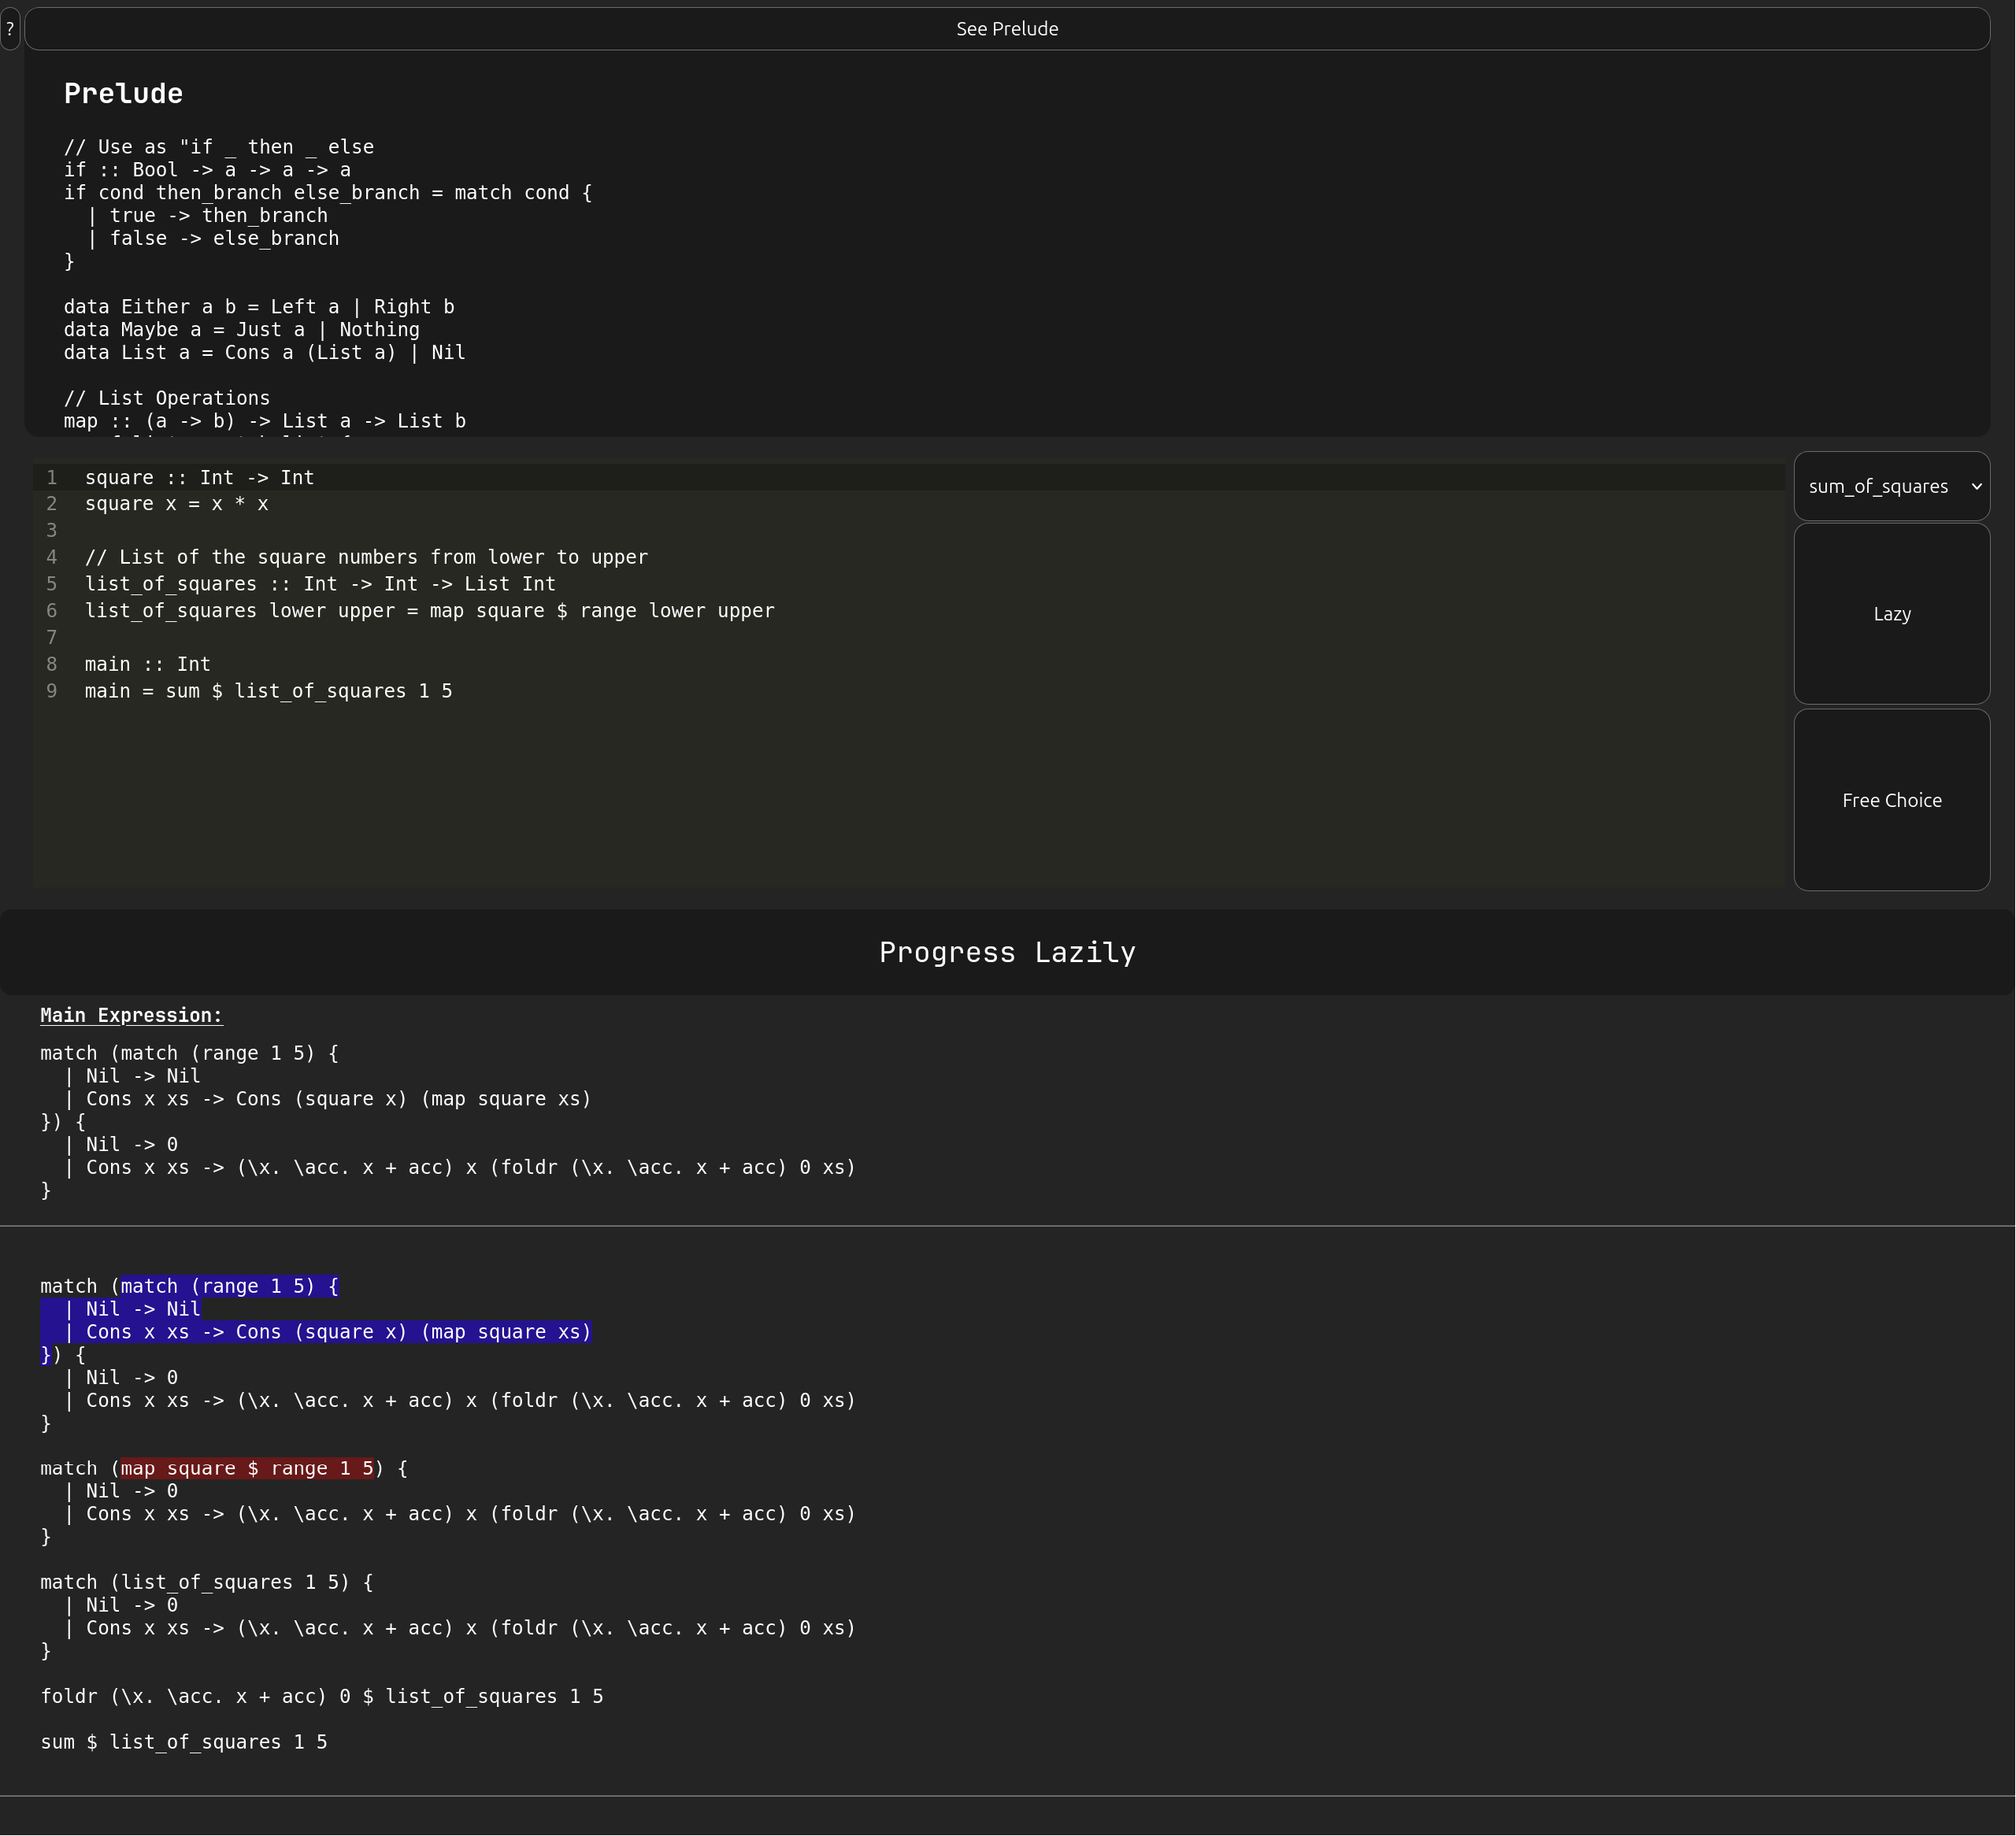
\includegraphics[width=1\linewidth]{images/phase-2-end2.png} 
    \captionsetup{justification=centering}
    \caption{The product at the end of phase two during lazy evaluation of the `sum of squares' sample program, with the prelude dropdown extended}
    \label{fig:screenshot_c2_end}
\end{figure}


\subsection{Changes to the Proof of Concept UI}
\label{c2_poc_ui_impl}
In this phase, I made some changes to the proof of concept web UI. See \ref{fig:screenshot_c2_end} and \ref{fig:screenshot_c2_end_free} for the desktop UIs, and \ref{fig:screenshot_phase2_mobile} for the mobile UI. 

\paragraph{Lazy Mode}
Added a separate `Lazy mode' which would only offer one button labelled `Progress Lazily'. The original functionality was included in `Free Choice' mode

\paragraph{History}
The history of the main expression is listed. The top two rows shows the most recent change, in blue is the result of the most recent change, in red is what it used to be. This does not work using the diff algorithm discussed in Phase 3 (\ref{paragraph:diff}), it instead gets the string before and the string after, and locates them in the second most recent and most recent program state. This is not fully accurate, as a string match results in false positives. If we reduced \sflinline{1 + 1} to \sflinline{2} in the expression \sflinline{(\x. x + (1 + 1)) (1 + 1)}, it would highlight both \sflinline{(1 + 1)}s even though the one in the abstraction has not been reduced. 

\paragraph{Other}

\begin{itemize}
    \item The prelude was offered as a dropdown.
    \item Some example programs can be loaded from a dropdown.  
    \item The program is saved in the browsers `localStorage' as it is edited
    \item A help menu was offered when the page was loaded, or when the `?' button in the top left corner was pressed: \ref{fig:screenshot_phase2_help}
\end{itemize}

\section{Testathon}
\label{c2:testathon}
The `Testathon' was an opportunity provided by the university for me and my fellow students doing dissertation projects to test our projects on each other, as well as other curious students in attendance. It was a valuable opportunity to test my system at the midpoint of the project. During the Testathon, I encouraged people to test the system on my laptop, as well as providing a QR code for them to be able to access it on their phone. I initially wanted to adopt a `think aloud' method for usability testing, which is `a method for studying mental process in which participants are asked to make spoken comment as they work on a task'~\cite{thinkaloud}

The plan was to implement this, and passively watch them interact with the system and not give them any extra instruction. However, I found that people required significant instruction. I attempted to delegate any instruction to the `help menu', but this did not solve the problem for the following reasons: people do not naturally want to read instructions, and my instructions were insufficient for people asked to interact with the system without any guidance to be able to effectively use it. Many people couldn't find the instructions, or were confused by the notation.

\subsubsection{Data Gathering}
After I explained the system and participants engaged with the system, participants were asked to fill out a survey. The results are included in the auxiliary materials~\ref{appx:additional_mats}. There were 15 participants, who were a mixture of undergraduate and postgraduate computer scientists, all of whom had taken the first year \ac{FP} unit. Participants were given some closed-form questions (see \ref{appx:Testathon} for an analysis of these results), as well as some more free-form questions:
\begin{itemize}
    \item `What do you like about the interface'
    \item `Do you have any things I can improve about the interface'
    \item `What do you like about the language'
    \item `Do you have any language features you think would make it better. I am intending to add pattern matching, so not that'
    \item `What do you like about the type system'
    \item `Anything I can improve about the type system'
\end{itemize}

The answers to these questions were mostly complimentary, but some useful information was extracted:
\begin{itemize}
    \item Participants appreciated the decluttered and simple UI. 
    \item They noticed that certain UI elements overflowed their boundaries, and that the UI had visual glitches on Safari.
    \item They found the help menu too long and wordy, and not clear or to the point enough.
    \item They liked the language, the type system and the inference. 
\end{itemize}

% I asked people who did not want to read the instructions to explain why, and their answers centred around the following points:
% \begin{itemize}
%     \item They could not find the instructions
%     \item The instructions look quite intimidating, due to being a large block of text
%     \item The instructions also look quite intimidating due to the unusual/unfamiliar pieces of syntax. This was in reference to the `Language Specification' section, and the `Types' section.
% \end{itemize}
% The first point did not provide any opportunity for further analysis, but the other points convinced me that a significant rework was needed to the UI and to the instructions menu. 

% I asked people needed further elaboration why they needed elaboration, and their answers centred around the following points:
% \begin{itemize}
%     \item The instructions contained quite a lot of `technical' language.
%     \item The instructions were not very good, and were incomplete, and often did not include new language features.
% \end{itemize}

% I could not gather data about other parts of the system, as I needed to explain the system in detail to everyone in turn, which did not allow me time to ask the questions I wanted to ask before people got bored and moved on. 

\subsubsection{Key Takeaways} The findings from the Testathon informed my future testing strategy:
\begin{itemize}
    \item The `Think aloud' method of watching people interact with this version of the system and asking them to narrate what they are doing is ineffective, as the UI is not `self-explanatory' enough for people to be able to use it without help 
    \item People do not want to read things. 
\end{itemize}

Certain visual glitches were also identified and fixed in phase 2. 

\section{The Advanced Focus Group: Evaluation and Next Steps}
\label{ref:afg_figma}
\label{ref:afg}
The aims of this phase were to develop the language as well as some other more technical features of this project. This was my first of three focus groups, the most advanced of the three. As the UI/UX was not polished at this stage, I wanted to find people who would be able to discuss the parts that I had already implemented to a reasonable level of completion: the language. However, I also wanted to discuss future steps for the system as a whole. Because of this, I identified people who had learned functional languages as a part of a university course fairly recently and within memory, so they would have an insight into what is required for the system to be useful for use in this setting. 

The transcript from this focus group is included in the Auxiliary Materials (see \ref{appx:additional_mats})

\subsection{Selection and Format}
For this focus group, I recruited four students in their fourth year of studies at the University of Bristol. I recruited outside of my immediate friendship group to try to prevent bias. They had all taken \hyperref[COMS10016]{the first-year FP unit} 3 years prior, and they had all taken units specializing in programming language theory since, including:

\begin{itemize}
    \item The second year Programming Languages and Computation unit COMS20007, where they learnt to (among other things) `Understand the interplay between the design and implementation of programming languages' \cite{COMS20007_PLC}
    \item The third year optional Types and Lambda Calculus unit COMS30040 where they learnt (among other things): \cite{COMS30040_TLC} 
    \begin{itemize}
        \item `Type systems: types, judgements and rules'
        \item `Syntax and semantics of an untyped lambda calculus'
    \end{itemize}
    \item The fourth year optional Advanced Topics in Programming Languages, where the unit outcomes were that they should be able to (among other things): \cite{COMSM0067_ATPL}
    \begin{itemize}
        \item `Specify the dynamics of program evaluation for a variety of programming constructs'
        \item `Specify static typing rules for a variety of programming constructs'
    \end{itemize}
\end{itemize}

These people I selected for this focus group were the closest to `subject experts' that I could find while still being undergraduate students. 
I started this focus group by briefly explaining. \ref{fig:screenshot_c2_end} shows how the system looked at this stage of the project. We also discussed the next UI iteration (see \ref{c2:next_ui}). 

\subsection{Outcomes}
The outcomes of the focus group are below, with timestamps to where the quotes can be found in the transcript: 
\subsubsection{The Language}
\paragraph{Positives:}
\begin{itemize}
    \item They liked the explicit match statements, and did not want me to change to more Haskell-like pattern match syntax: 
    
    `Stick with the match expressions because it's very clear that matching has happened when you have the word match there' [Participant 2, 24:11]
    \item They liked that \sflinline{Cons} was a prefix constructor rather than infix: 
    
    `I think it's good that Cons is a prefix, like a normal constructor, and not a colon or
    something like that' [Participant 4, 17:41]. 
    \item Similarly, they liked the limited set of operators, and the fact that you cannot define your own: 
    
    `I think if I was learning functional programming for the first time, I would really hope there aren't custom operators' [Participant 3, 15:56]
    
    `If I'm trying to learn functional programming, I don't think it helps me to be able to define, like, things that have different precedents. I think that distracts from learning how programs are reduced' [Participant 4, 16:42]
\end{itemize}

\paragraph{Negatives/Potential Improvements:}
\label{ref:afg_ite} 
Sentiment about the language was good, the only language specific issue was that they were confused about if-then-else syntax. They said it could be confusing to have the parser act differently for one specific function type. 

`The issue I was having is just the fact that there is a function in the prelude which has the same name as some syntactic sugar that is a parser construct' [Participant 2, 42.55]

\subsubsection{The Existing User Interface, and the System as a Whole}
\paragraph{Positive}
They really appreciated its utility for what it was designed for. Most of what we discussed was potential improvements rather than positives of the proof of concept system, however they seemed engaged and excited despite not being explicitly positive about it, beyond this one comment:
    
\begin{quotation}
\noindent `I think this is very good \ldots\ I wish I'd had this in the functional labs' [Participant 3, 1:00:09]
\end{quotation} 

\paragraph{Negatives/Potential Improvements:}
\begin{itemize}
    \item `Syntax highlighting would obviously help' [21:45]
    \item They were confused as to why, in free choice mode, some reduction options included each other: 
    
    `The first one is a chain of reductions that contains the second one. I think it's fine to display that as long as you make it visually distinct that these two are related in that way and the other reductions are just independent' [12:57]

    This could be implemented by having a dropdown where the highest level one shows all the ones below it. 

    `You could put a number next to the reduction and say, you know, this is four steps. And then \ldots make a drop-down. Yeah. So if someone wants to see what steps are going on inside there, then they could see' [08:57]
    \item They wanted an indication of which direction evaluation was going: 
    
    `Because the reduction steps generate bottom-up, it might be good to have some sort of indication about the direction things are going in' [28:12]. This was already in the new UI, which had not seen by this point in the transcript.

    \item They wanted to be able to hover over an option and have it highlight what would change: 
    
    `I think one thing that is not immediately clear is how the different reductions you see are related to the main program. If there was some way that like if you hovered over one, you could highlight the portion of the program that it corresponds to' [10:28]
\end{itemize}

\subsubsection{The Next Iteration UI Design}
\paragraph{Positives:}
\begin{itemize}
    % Make sure this stays with the prev one about reduction steps
    \item The new UI included indication of which direction evaluation was going, see above. 
    \item They liked the ability to revert progress: 
    
    `Something I had not thought of, very good' [54:59]
    \item They liked the horizontal split: 
    
    `It's easier to have everything on screen and it's more akin to what people may have experienced' `Its like compiler explorer'. [52:38] `I think immediately not having to scroll is a massive plus' [52:58]
\end{itemize}

\paragraph{Negatives/Potential Improvements:}
No improvements were discussed for the next UI specifically, but most of the potential improvements for the current UI apply. 

\section{Phase 2 Conclusion}
Phase 2 resulted in a programming language which has syntax, semantics and a type system that are fit for purpose. I tested the project on 19 people in total - 15 in the Testathon and 4 in the advanced focus group. The language was very popular with the Testathon users as well as the Advanced Focus Group. There were no specific complaints about the language from either group. 

The proof of concept UI had mixed feedback. During the Testathon~\ref{c2:testathon}, people cited its `cleanness' i.e. lack of overcomplicating buttons. However, people did not like having to scroll to refer to the original program, and the confusing nature of the way the history was generated bottom up with no indication of direction. 

The advanced focus group also had a lot of feedback on how to improve the UI and language. The new UI as designed at the beginning of phase 2 \ref{c2:next_ui} was popular with the Advanced Focus Group. They had no specific thoughts on how to improve it, however they had many thoughts on features that could be added to the UI and the system as a whole in order to make reduction clearer. 

By the end of the project, I implemented the new UI along with syntax highlighting, and many other clarifying features. 

However, I unfortunately did not have time to work on grouping related reductions together or highlighting in source code when a progress option is hovered over what it would change, or improving the help menu. See the `future work' section \ref{conc:future_work} for more detail. 
\chapter{Phase 3 --- Improving the UI/UX}
Phase 3 was the first of the two shorter phases focusing on UI iteration. It spanned approximately two weeks, starting with the implementation of the new UI, and ending with the second of the three focus groups with first year undergraduate students. 

\section{Requirements Analysis}
The motivations for this phase come mainly from the advanced focus group, however requirements from the \hyperref[sec:c1_autoethnography]{autoethnographic phase} of the project, as well as the \hyperref[eval:c1]{proof of concept client meeting} continue to be relevant. 

The advanced focus group was generally very positive about the language, but they had many thoughts about the Proof of Concept UI they were presented with. During phase 2, I created a Figma prototype for the next UI (see \ref{c2:next_ui}). Many of their thoughts about the Proof of Concept UI were things that were already addressed with the new design. This prototype was presented to the advanced focus group, who much preferred it. The advanced focus group had no criticism of the new UI, so it should be implemented as designed for now. 

The prototype for the new UI also included the functionality to `undo progress', by clicking on a previous program state in the table to make this the current version of the program. The advanced focus group appreciated this functionality. 

% \section{Design}
% Because I wanted to be able to evaluate the prototype for the web UI with the advanced focus group, the web UI was designed in the last phase. I set aside time to design 


% \todo{there was no design here? the advanced focus group liked the protype a lot and did not have any }

\section{Implementation}
Implementing the new UI mostly consisted of time-consuming React and CSS tweaks which are not worth mentioning here. However, there were some more challenging aspects that required some more interesting considerations and changes to be made. Screenshots of the result of implementing the new UI with these features is shown in \ref{screenshot:phase3_end_lazy}, with another example showing free choice evaluation in the appendix \ref{screenshot:phase3_end_free}. 


\subsection{Diff}
\label{paragraph:diff} 
Our frontend requires the ability to see what has changed between two program states. Highlighting these changes make understanding the changes in the users program in the frontend easier. This function generates the strings for the two trees simultaneously, producing the similarities and differences. If two nodes are different structures, then we turn them into strings and regard them as differences. However, if two nodes are the same structure, we identify what parts of that structure are similarities and what parts are differences. For instance, if the algorithm is called on an application, we generate the diff for the function and for the argument separately, and then concatenate the diffs. \ref{fig:diff_list} shows a subsection of this algorithm, showing how it works for IDs, Literals and Pairs. 

% Move to c4
% \subsubsection{Syntax Highlighting}
% \subsubsection{Display RC history}
% We also wish to         

\subsection{Reduction Messages}
Rather than presenting the user with simply the before and after of the reduction, this design calls for presenting the user with a message describing what will happen. While generating the options for reduction (see \ref{c1_design_reduction_progress}), we can keep track of information relevant to how it was generated to inform the message displayed. For instance, if a reduction is generated from the application of a named function with name A to two arguments B, C, we can convert those arguments to strings and then broadcast the message `Applied function A to B and C'. 

If B or C are large pieces of syntax, this may generate a very large unintelligible string. To solve this, we can modify our stringification algorithm to do certain things different to normal:
\begin{itemize}
    \item Do not show the cases of a match statement, as the condition should be enough differentiate it
    \item We can truncate the output to a fixed length 
\end{itemize}

In past iterations, redex-contraction pairs were passed to the front end as two strings. We can make it three strings instead, where one of the strings is the reduction message which can be displayed before the reduction. The other two strings, the redex and contraction, can be displayed after the reduction in the history. 

\subsection{Revert Progress Functionality}
We may wish to undo progress. This was functionality designed into the new UI that the advanced focus group specifically mentioned liking. 

Undoing progress requires that previous \ac{AST} states must be stored. Before now, the most recent \ac{AST} state was stored at a known memory address so any of the functions in the binary could know where to find it. This was done to avoid having to pass the \ac{AST} to the JavaScript module. If we wanted to store the history of all \ac{AST}s, one approach could be to store all the \ac{AST}s in a pre-allocated memory region in a stack, and then allow the JavaScript module to refer to each of the \ac{AST}s in the history by their stack index. However, pre-allocating enough memory for any potential program execution logs would be misguided, as it would cause accessibility problems for computers with less memory. Instead, we should employ dynamic allocation. 

The issue with dynamic allocation of memory for the \ac{AST}s as they are added to our history is that we no longer know exactly where they will be located, meaning this information must be stored such that it will not be erased between calls to \ac{WASM} library functions. One method of doing this is passing a pointer to where in memory the \ac{AST} is located to the JavaScript module so that it can refer to it later, and use library functions on it. At first glance, this sounds like a bad idea, as when pointers are returned from a function for which wasm-bindgen (see~\ref{bg:wasm-bindgen}) is used to make a JavaScript binding, the pointer is represented as a JavaScript $number$ type~\cite{wasm_bindgen_guide}, which is a double-precision IEEE-754 value~\cite{ecma262number}. Storing pointers as floating point values, and then attempting to dereference them, sounds like a recipe for memory mismanagement. However, this is safe because WebAssembly 2.0 has 32 (see~\ref{bg:wasm}), and thus has 32 bit pointers, and a double precision floating point number has a 52 bit~\cite{ieee754} mantissa meaning it can safely store the 32-bit memory location without issue. 

In our JavaScript module, we can then store a stack of pointers to the \ac{AST}s, and display the options for reducing the one at the top. When an option is selected, we can apply the reduction and then store the new \ac{AST} on the top of our stack and recalculate reduction options. If the user decides to start evaluating a new program, all the \ac{AST}s with pointers in this list are freed to avoid memory leaks.

\begin{figure}[h]
    \centering
    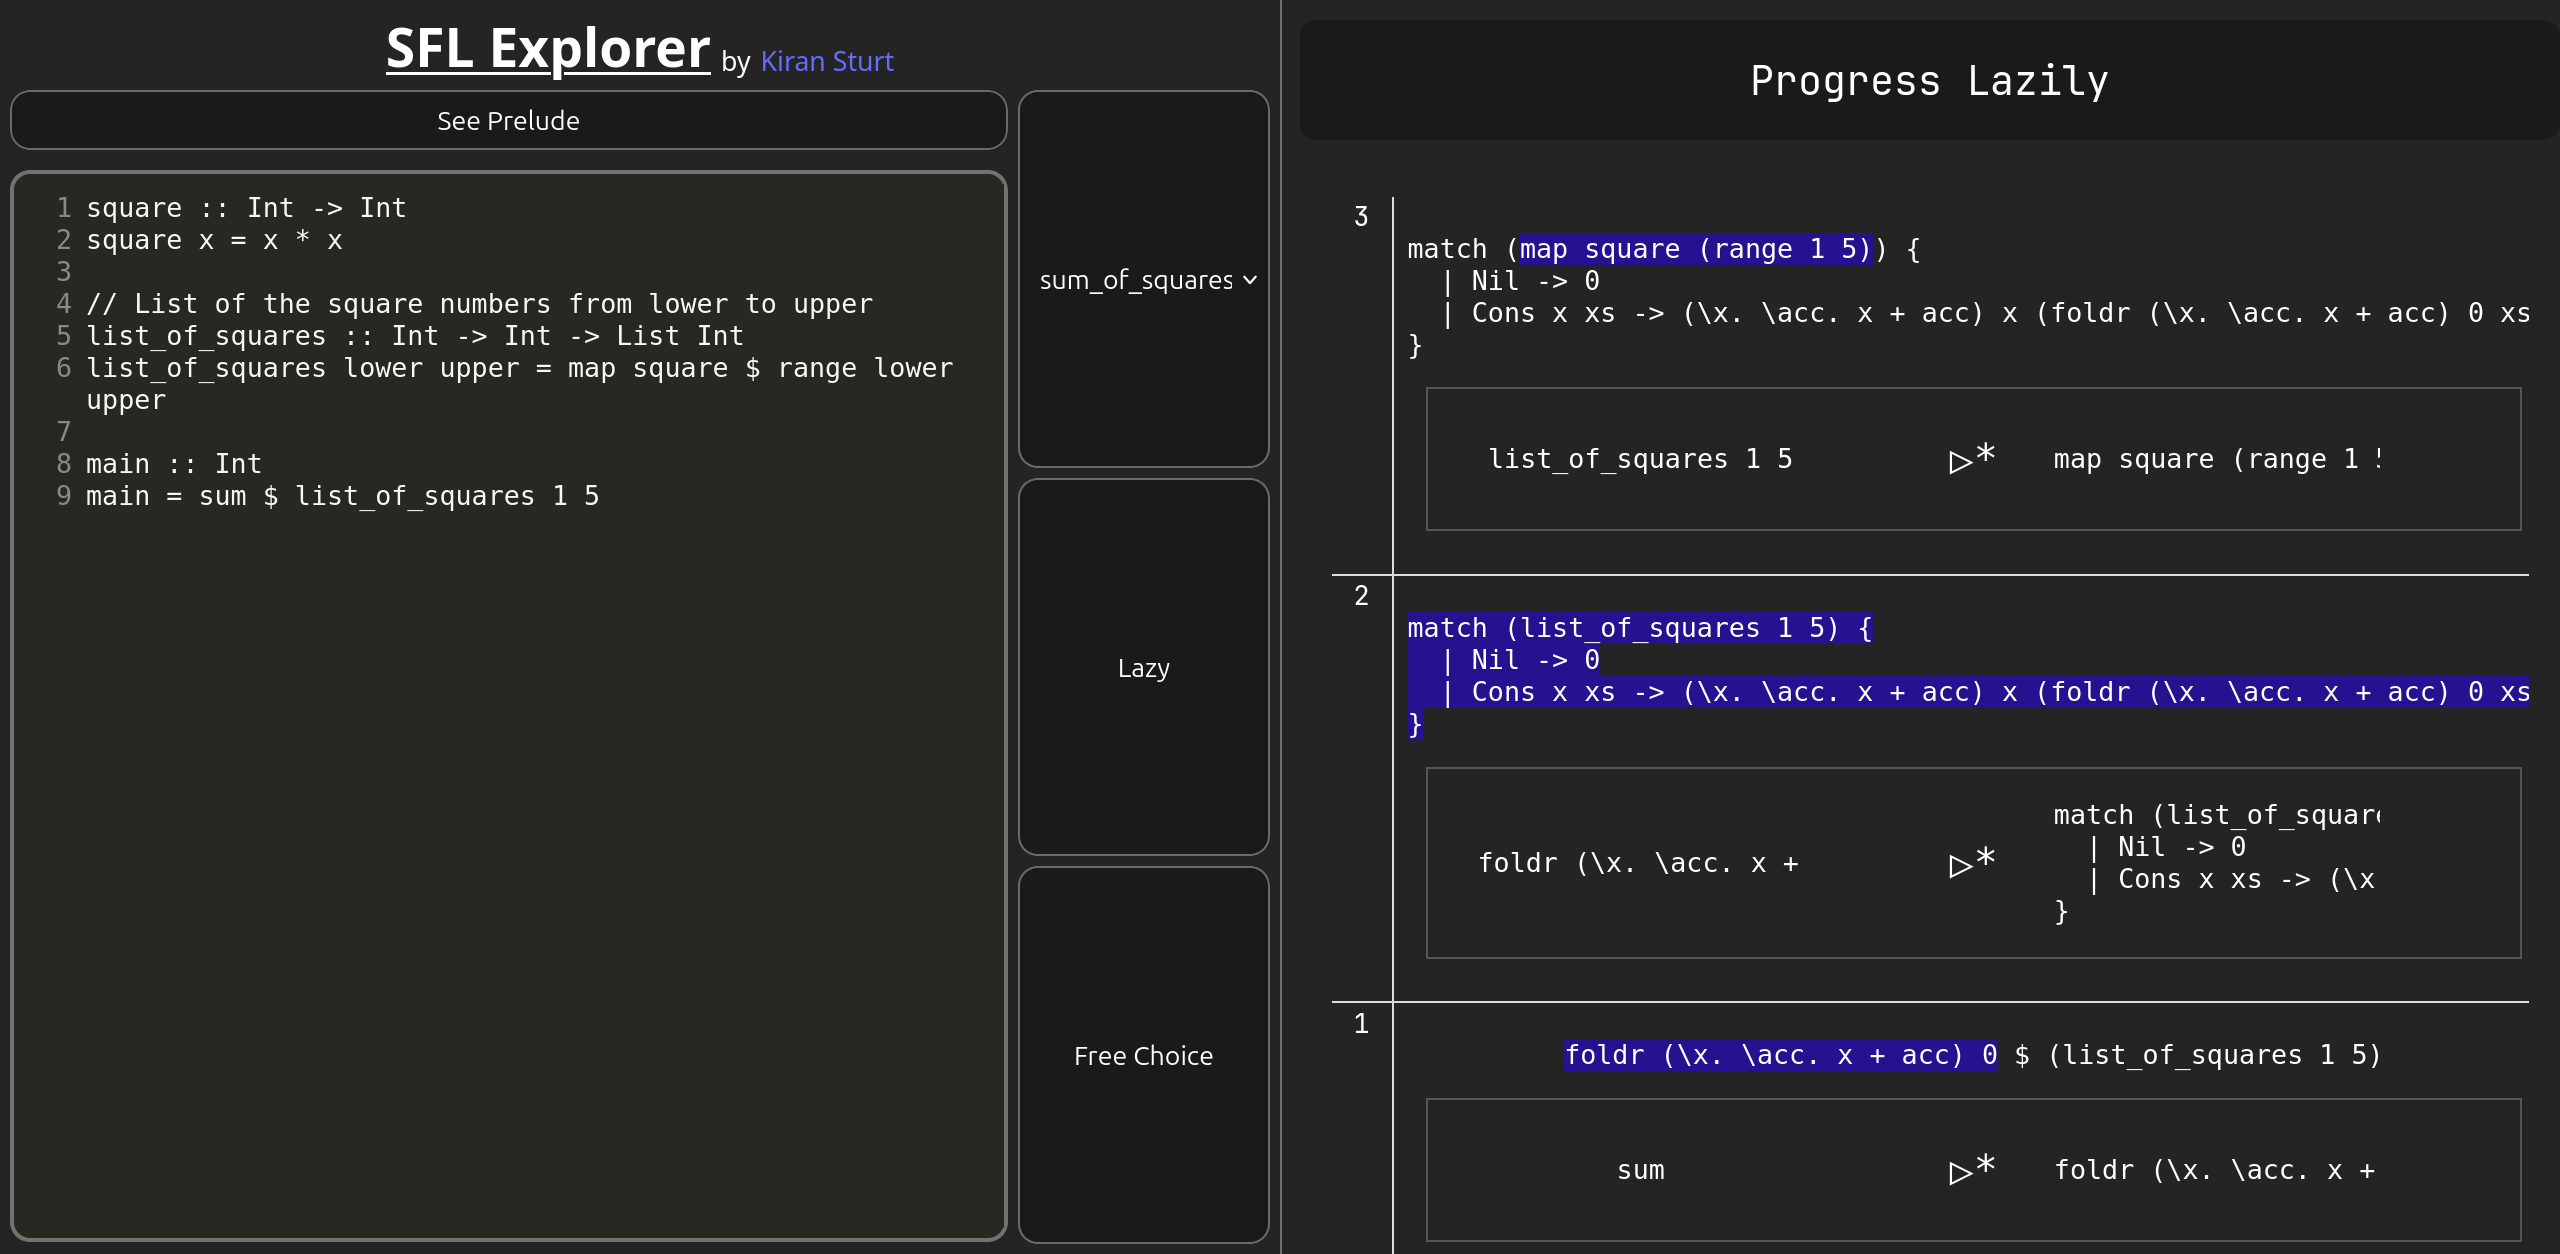
\includegraphics[width=\linewidth]{images/phase-3-end.png}
    \caption{The new UI implemented, during lazy evaluation of the provided `sum of squares' example program}
    \label{screenshot:phase3_end_lazy}
\end{figure}

\section{The Intermediate Focus Group: Evaluation and Next Steps}
\label{eval:IFG}
The Intermediate focus group happened at the end of phase 3 of the project. An entirely different structure was employed for this focus group than the Advanced Focus Group \ref{ref:afg}, as the aims of this focus group were different. Rather than just evaluating the language, I wanted to evaluate the system in the setting that I expected it to be used in: a lecture setting. 

To act as a lecturer, I employed Amos Holland, a fourth year undergraduate student. I considered doing it myself, but I decided that it would be better to employ an undergraduate who was more experienced in teaching functional programming. Amos was selected as he had taken all of the functional programming units that were available in his degree so far: the same ones that the participants of the Advanced Focus Group had taken (for details of these units, see \ref{ref:afg}). Furthermore, Amos had acted as a teaching assistant on two of these units, Types and Lambda Calculus, where he ran weekly problem classes, where he would walk students through difficult problems from the lectures or worksheets, and \hyperref[COMS10016]{COMS10016} where he had been a teaching assignment working in labs in the same capacity as I had. 

\subsection{Selection and Format}
For this focus, to evaluate SFL explorer as a teaching tool and get feedback, I selected first year undergraduate students who had just taken the functional programming unit. I looked for people who had not explored functional programming outside this unit, and who found the unit difficult, as these are representative of group of people the tool would be most useful for. 

\subsection{Bugs}
There were numerous bugs that Amos and I identified during the lecture phase of this focus group:
\begin{itemize}
    \item The editor would sometimes add tab spaces randomly.
    \item Sometimes, the site would refresh on its own.
    \item The editor did not save input consistently.
\end{itemize}
\noindent These were all fixed as part of phase 4.

\subsection{Outcomes}
Due to technical issues, I was only able to get a transcript of the interview portion of the intermediate focus group; I made the mistake of holding this focus group in a room where there was too much background noise to get a high quality recording during this part of the session. However, during the interview, I set up multiple microphones, and was able to combine the AI transcripts from each of them into one transcript. The transcript is in the additional materials \ref{appx:additional_mats}. 

Below is the summary of outcomes from the discussion with this focus group, along with timestamped quotes where relevant. The first phase of this interview was conducted with Amos, followed by an interview with each participant in turn. 

All four participants, and Amos, liked SFL explorer as a whole. 
\noindent\begin{quotation}
\noindent`I think it was good, other than the few bugs' [Amos, 00:04]
\end{quotation}
\noindent\begin{quotation}
\noindent`Yeah, I liked it; this is what I do in my head basically when I'm looking at Haskell, it [the lecture using the tool] was good' [Participant 1, 06:44]
\end{quotation}
\noindent\begin{quotation}
\noindent`I really like what the tool does, like it
shows like what you can see because that's basically what I do when I'm like debugging code but
um it takes like a long time to do it like by hand and to go through everything and sometimes it's
like wrong if you do it yourself so this is like a good way to automate it' [Participant 2, 15:20]
\end{quotation}
\noindent\begin{quotation}
\noindent`I liked it' [Participant 3, 19:07]
\end{quotation}
\noindent\begin{quotation}
\noindent`I actually really love the functionality of this app' [Participant 4, 24:44]
\end{quotation}


In the Advanced Focus Group outcomes section \ref{ref:afg}, I split the focus group's thoughts into positives and negatives. However, in this focus group opinions were more split between participants, as well as participants being more frequently in two minds, so I did not do this. Instead, I have grouped by topic rather than by positivity and negativity, so one bullet point may have both positive and negative thoughts towards the same issue. 

\subsubsection{The Language}
Below is the summary of Amos's and the participants' thoughts about \ac{SFL}, along with timestamped quotes where appropriate.
\paragraph{Amos}
\begin{itemize}

    \item Amos liked the explicit match statement:
    
    `I quite like match, because I think it gets a bit more directly at what pattern matching is doing, like that it's a specific operation' [03:36]

    \item Amos was happy with the language and its features
    
    `There are features of Haskell it doesn't have, but Haskell is a very advanced language. For teaching functional programming, I think it's got the right range of features' [Amos, 00:04]

    \item Amos identified adding type classes as a potential next step 
    
    `If you were to take this, like, a step further, make it more advanced, I think the next step is type
    classes' [Amos, 00:04]
    
    \item `I like the stuff we put in the prelude because we have like sort of basic functions' [Amos, 00:04]
    
    
\end{itemize}

\paragraph{The Participants}\begin{itemize}
    \item They had mixed opinions on whether I should add the usual syntax sugar for lists. Below are two quotes from two participants, showing their split minds on this topic:
    
    `I both love and hate the list, the lack of syntactic sugar for list, \ldots it makes literal lists really hard to read, but it makes the types so much clearer. Having to interact with that rather than just going, that's kind of an array \ldots It really explicitly forces you to think in the Haskell
    way' [Participant 1, 14:47]
    
    `I really liked that, like, well, because we don't have the constructor we had in Haskell
    for, like, lists. Abundantly much clearer to me what was going on \ldots I prefer it with this list, this cons and the nil. But also you have to write it out for five hours as the teacher' [Participant 3, 22:52]

    \item They liked the explicit match statements. 
    
    `I honestly really liked the match being, like, write match. Yeah. So the
    explicitness was good. I really liked that. It made it obvious to me in a way that it wasn't necessarily before \ldots\ This is much easier to learn about pattern matching with than Haskell' [Participant 3, 19:07]
\end{itemize}

\subsubsection{The User Interface, and the System as a Whole}
An absolutely critical issue that became obvious during the focus group was the need for a light mode. The room was very bright, and it was barely visible in dark mode. This was resolved with a high priority in the next phase. 
Below a more detailed summary of their thoughts about SFL Explorer as a whole, and the UI/UX:

\paragraph{Amos}\begin{itemize}
    \item Amos was generally happy with the UI for teaching.
    
    `As far as the design went, I think I was happy with it for teaching' [Amos, 00:04]
    \item A `step to the end' options would be good, allowing the user to complete evaluation without having to click on the button many times.
    
    `It would have been nice to have a button that says steps to the end, because there were some cases where I would have liked to just see if it evaluated correctly, but
    instead you had to click through a lot of times' [Amos, 00:04]
    \item Amos wanted to be able to save more programs than just one.
    
    `It would be nice to be able to define more complete programs and save them so that you can jump between them a bit' [Amos, 02:57]
\end{itemize}

\paragraph{The Participants}\begin{itemize}
    \item They wanted syntax highlighting, indeed 3 out of four explicitly asked for it. 

    \item Two of the participants agreed that the history should be shown in reverse, so it would generate top down, the other two did not comment. 
    \item One participant specifically mentioned liking the way the UI separates the editor from the output
    
    `I like that it's separate. Text editor here. Then this bit shows what it does' [18:02]
    \item They liked how it highlights what has changed between iterations:
    
    `I really like the highlighting in like what changed' [Participant 2, 15:20]
    
    `I, like, as a minor visual thing, \dots\ like, you have the blue bit of the bit you've changed on the right-hand side' [Participant 3, 19:07]
\end{itemize}


\section{Phase 3 Conclusion}
This phase resulted in a high quality UI that was much more polished than the previous iteration. The UI was generally popular with the focus group, and the language continued to be well liked. However, there were many ideas for improvements to be made, the clearest one being adding a light mode. 

% The aims of this focus group were to use the system and attempt to recap functional programming concepts 

% Evaluation:
% - They liked explicit match: they liked it more than haskell for learning about how pattern matching works
% - Really Really needed light mode
% - Horizontal overflow bug
\chapter{Phase 4 --- Further UI/UX Iteration}
\section{Requirements Analysis}
This phase was limited by time, as the project was nearing its end. For this reason, this phase was mostly focused on fixing the high priority issues identified in the previous phase. This included adding a light mode, adding syntax highlighting, as well as fixing language and typechecker bugs. 

At the end of this phase, I wanted to hold another focus group where Amos would give a lecture on functional programming, but this time to complete beginners. After a planning conversation with Amos at the beginning of Phase 4, we identified that it would be useful to add an `untyped mode' so the beginners could be taught the basics of \lcalc\ before trying to explain types, as they can be initially confusing. 

\section{Design and Implementation}
\subsection{Syntax Highlighting}
In order to implement syntax highlighting, I found the source code for the Haskell syntax highlighting supported by the library I was using for my editor (\href{https://codemirror.net/5/}{CodeMirror 5}). I edited this with SFL's syntax and keywords. Syntax highlighting was also applied to the prelude to make it easier to read. 

\subsection{Light Mode, and the Settings Menu}
The `light mode' colour scheme was designed by returning to the room where the Intermediate Focus Group was held on a day with similar amounts of sunshine, and testing different colours for visibility. The light mode scheme also had different syntax highlighting from dark mode. 

To implement it, I added a floating settings menu with a button that would toggle from light mode to dark mode. This worked by adding or removing the class `light' from the top level HTML element, where all elements descending from this node would be in light mode if it was set. I also added a button for toggling `untyped mode', as well as toggling whether the prelude was included. These settings would be saved in the user's browser.

Using CSS media queries, I was also able to tell the user's preference for light or dark mode from their browser, and use this by default unless the user chose otherwise. 

\subsection{Bugfixes}
\subsubsection{Frontend}

\section{The Beginner Focus Group: Evaluation and Next Steps}
\label{eval:BFG}
\subsection{Selection and Format}
This focus group had the same format as the intermediate focus group \ref{eval:IFG}; Amos was employed once more to give a 45-minute lecture, followed by a 45-minute interview. The full transcript of the lecture and interview is available in the additional materials \ref{appx:additional_mats}.

The goals of this focus group was to evaluate the use of SFL explorer in a lecture setting with complete beginners, with a wide variety of different experiences and perspectives on programming. Crucially, I wanted none of them to have learnt about or used functional languages before. As such, I decided to recruit non Computer Scientists. Hoping to get a mix of more `practical' and more `theoretical' students, the four students I recruited were from the following disciplines:

\begin{itemize}
    \item A second year undergraduate Mechanical and Aerospace Engineer from the University of Cambridge, with experience in Python
    \item A third year undergraduate Mechanical Engineer from the University of Bristol, with experience in Python and C/C++
    \item Two third year undergraduate Maths students from the University of Bristol, with experience in mostly Python and R
\end{itemize}

\subsection{Bugs}
There was a bug where the type checker would not correctly follow type aliases, causing crashes in a program with type aliases. This was fixed afterwards. 

\subsection{Outcomes}

\subsubsection{The Language}
Participant's did not have many comments on the language, as they had never seen a functional language before, so they couldn't really compare. 

However, Participant 2, a Maths student, in particular seemed excited about functional programming as a concept:
\begin{quotation}
\noindent `It's cool to see a language that's like, I don't know, I feel like if I was going to do some maths in my head, this is how I'd actually do it' [Participant 2, 01:05:22]. 
\end{quotation}
\noindent Participant 2 also asked several questions about the history of functional programming, showing their engagement. 

Participant 1 was confused about the bar character used to separate cases in a match statement, as it was the same as the character used to separate tagged union variants. 

\subsubsection{The User Interface, and the System as a Whole}
Most of the feedback was positive, and users had no specific feedback on what they would like to see be changed in the system. 

\begin{itemize}
    \item Two participants said they preferred dark mode, but both agreed light mode is important to have.
    
    \item Free choice mode was very popular, with two participants specifically mentioning when asked for things they liked in the system. 

    \item Participant 3 really liked the interface, and found the session particularly interesting:
    
    `I really like the coding part and the sections on the right, in terms of seeing how it goes from one to another. I think that was really useful. In terms of learning it. Yeah. And the free choice variation. I also agree that it shows nicely what the functions are actually doing' [Participant 3, 01:03:11]

    \item Participant 2, a Maths student, was very positive about the UI and the tool:
    
    `I think you've done a really good job of making it quite beginner-friendly because it's all quite easy to read' [Participant 2, 01:06:05]

    \item `UX is very intuitive' [Participant 1, 01:12:07]
\end{itemize}

\section{The Final Client Meeting}
\label{c4:client}
\todo{This bit}
After the beginner focus group, I met my client. This was at the end of the project

My client liked my project, and shared it with Jamie Willis, a teaching fellow at Imperial College London, who is involved in their first year unit which includes functional programming \cite{imperialFP}. When my client asked about whether he would use it, he responded:

\begin{quotation}
\noindent `I could see it being useful for sure, a lot of the time I end up writing out these step-by-step reductions by hand in my notes, but it would be nice for them to have access to a tool they could use to explore for themselves'
\end{quotation}

% `Wait, is SFL your language? It was so good that i just assumed you had grabbed it from somewhere'

% The aims of this focus group were to use the system and attempt to recap functional programming concepts 

% Evaluation:
% - They liked explicit match: they liked it more than haskell for learning about how pattern matching works
% - Really Really needed light mode
% - Horizontal overflow bug

% A/B testing different schemes with some of my fellow undergraduates, as 

% The changes to the UI were time-consuming but not worth mentioning here. 
% \chapter{Design}
\label{chap:design}

\section{Language Design}
\subsection{Goals}
\label{design:goals}
SFL is designed with the following goals in mind:
\begin{enumerate}
    \item SFL should be similar to existing functional languages.
    \item SFL should be simple and easy to understand. 
    \item SFL should be powerful.
\end{enumerate}
The features that should be selected for SFL are the features that maximise these goals for the minimum implementation complexity. The language's syntax and type system should also work towards these goals. 

Out of our design goals, 2 and 3 have the potential to be in conflict, as more expressive power often requires more complex syntax. We must ensure a sensible compromise between all of our goals, while accounting for implementation complexity. 

When adding features for the language, we must prioritise the "core" features of functional languages, and de-prioritise features that are not so "core" to the understanding of functional languages. 

yadadada we should implement features that allow us to implement
\begin{itemize}
    \item Complex data structures, lists and trees
    \item Fold
    \item IO???
\end{itemize}

\subsection{Definitions}

\begin{syntax}[Lowercase and Uppercase ID syntax as regular expressions]
\label{def:identifier_syntax}
(Lowercase Identifier): \(id ::= [a..z][a..zA..Z0..9\_]*\)\newline
(Uppercase Identifier): \(Id ::= [A..Z][a..zA..Z0..9\_]*\)
\end{syntax}

\subsection{Basic Syntax}
Lambda calculus is the basis of modern functional programming languages. As discussed in the background, Lambda calculus consists of 3 structures: identifiers, application, and abstraction. One common extra structure that functional languages implement is an assignment. This is where we label an identifier with a certain meaning, such that all references to the assignment henceforth are identical to a reference to the meaning assigned. For instance:
\begin{lstlisting}[]
f = (\x.x)
main = f y
\end{lstlisting}
Is identical to
\begin{lstlisting}[]
main = (\x.x) y
\end{lstlisting}
Note the use of \verb|"\"| instead of \(\lambda\) as it is the closest character available on most keyboards. A program is then defined as a set of assignments, and we pick one specific label name to mark the "entry-point" expression in the program. Haskell, as well as many other languages, use "main" to represent a programs entry point, so we may use main. 

We must also add a way to represent values, such as integers and booleans, to our language. Most programming languages, including functional ones, at least support integers. Booleans are also often supported to represent the results of integer comparison. Without literal values, programs would have to use complicated encodings (such as church numerals) to represent these values, making programs look more complicated. 

These two features massively shorten and simplify programming in this language.

\begin{syntax}[The basic syntax of SFL]
(Expression) \(E ::= [-][0, 1, ..] \mid true \mid false \mid id \mid \setminus id. E \mid E\:F\)\newline
(Assignment) \(A ::= id = E\)\newline
(Module) \(M ::= A\: M \mid End\)
\end{syntax}

\subsection{Type System}
We must have types representing integers and booleans in our language, if we are to effectively check the validity of expression containing their respective literals. 

Many languages, including Haskell, also have Algebraic Data Types allowing us to "Compose" other data types. Algebraic data types are isomorphic to an algebraic expression consisting of sums and products of their constituent types. An example of a product type is the tuple \((Int,Bool)\) which is isomorphic to \(Int \times Bool\). Most languages have product types, which often take the form of structs or tuples. 
An example of a sum type is the Haskell syntax tagged union:

\noindent\verb!"data Shape = Circle Int | Rectangle Int Int"!, which is isomorphic to the type \(Int + (Int \times Int)\). 

We will now consider generic data structures, such as a lists that can hold any value of type $a$, written as \(List\;a\)". Here, \(List\) is not a type in itself, but it represents a constructor that takes a type, and returns a concrete type. We could write this as "$Type \rightarrow Type$", indicating that it behaves like a function, but at the type level rather than the value level. If we were to apply the constructor \(List\) to the concrete type \(Int\), the resulting type would be \(List \;Int\). 

Polymorphism as described here is first order polymorphism, as opposed to higher-order polymorphism (also known as higher-kinded polymorphism) where a type can abstract over a type that abstracts over a type \cite{pierce2002types}. An example of a function that is higher-order polymorphic is a function that takes a function, and then applies it to two differently typed values:
\begin{lstlisting}
applyToBoth f x y = (f x, f y)
\end{lstlisting}
If \verb|f| is to be applied to any type, it must have a type \(\forall a. a\rightarrow a\). This means the type of the function \verb|applyToBoth| must be \(\forall a \;b.(\forall c \rightarrow c) \rightarrow a \rightarrow b \rightarrow (a, b)\)

This requires the ability to parse expressions with nested \verb|foralls|, as well as support during type inference for higher-kinded types. We do not think that this is a priority for the system, as 
These first-order polymorphic type constructors would be useful to have in SFL, with one example of their utility being defining the polymorphic function "\verb|length :: List a -> Int|" which should work regardless of what type the list is over. Higher order polymorphism is less important
The "Type of a Type" is known as its \emph{kind} \cite{pierce2002types}. Another example is the type representing "Either left or right: \(Either \;a\;b\)", that can be defined with its constructors as \verb!data Either a b = Left a | Right b!. "Either" is a type constructor with the kind "Type -> Type -> Type", meaning it takes two concrete types and returns a concrete type. 
Higher-kinded types are types where there are parenthesis in a kind expression, not including the implicit ones implying right associativity: 
"\verb|Type -> Type -> Type|" is implicitly "\verb|Type -> (Type -> Type)|"
We can avoid thinking about kinds by enforcing that a type constructor is always given the correct number of arguments

Supporting tagged unions and tuples in the SFL type system would massively increase the ease of writing complex programs. It would also allow for complex data structures such as trees and lists. 
Type names, as well as constructor names, start with uppercase letters in Haskell. This allows them to be easily differentiated from type variables, as well as regular variables. 
In the below definition of the SFL type system, we define \(\Alpha\) as the set of valid type names starting with uppercase letters defined by \(Id\), and \(\alpha\) as the set of valid type variable names defined by \(id\). 

\begin{syntax}[Types in SFL]
(Inbuilts): \(B::=Int\mid Bool\)\newline
(Monotype): \(\tau, \sigma ::= \alpha \mid B \mid \tau \rightarrow \sigma \mid (\tau, \sigma) \mid \Alpha \;T, U,...\)\newline
(Alias): \(A ::= Id = T\)\newline
(Type): \(T, U ::= \alpha \mid B \mid T \rightarrow U \mid (T, U) \mid \forall a. T \mid \Alpha \;T, U,...\)
\end{syntax}
Note that our type constructor application definition above is more permissive than is correct, as it does not enforce correct arity. This can be handled by the parser maintaining the context of the arity of each type. It can then be double checked for debugging purposes via an assertion in the type checker. 

\subsection{Match}
To support different execution based on a condition, we must have some structure that can differentiate between values \ref{design:values}. 

\subsection{Syntax Sugar}

\subsection{Reduction}
Functional programs progress via reduction. 
\paragraph{Values}
\label{design:values}
% \chapter{Implementation}
\label{chap:execution}


\section{OLD PARSER BIT}
\subsubsection{Parsing Match Statements}
An example of using a match statement follows:
\begin{verbatim}
lengthIsAtLeast2 list = match list {
  | Cons x (Cons y xs) -> true
  | _ => false
}
\end{verbatim}

The algorithm used for parsing match statements is:
\begin{itemize}
    \item Consume the "match" keyword.
    \item Parse the expression matched over
    \item Consume an open brace
    \item While the next token isn't a close brace: \begin{itemize}
        \item Parse a pattern (\ref{impl:parsing_patterns}).
        \item Consume a right arrow
        \item Parse an expression
    \end{itemize}
    \item Consume a close brace
\end{itemize}
Following this, a match node is created, where the \verb|children| vector is set appropriately with the pattern and expressions.

\paragraph{Patterns}
\label{impl:parsing_patterns}
A pattern must be a value \ref{design:values}; a pattern must not contain anything that can be reduced. It would be nonsensical to have a situation where we had a pattern not in normal form such as \verb|1 + 1| and the expression to be matched was \verb|2|. 

To parse a pattern, we may use the same techniques as parsing an expression, with a few differences:
\begin{itemize}
    \item Disallowing abstractions
    \item Identifiers must be either:
    \begin{itemize}
        \item Unbound lowercase variables
        \item Underscore (\verb|_|) representing a wildcard pattern
        \item A bound uppercase variable (a constructor)
    \end{itemize}
\end{itemize}



\subsection{Module Parsing}

\section{Type Checking}

\section{Identifying Redexes}


\section{The CLI}


% \chapter{Critical Evaluation}
\label{chap:evaluation} 
% \chapter{User Testing}
\label{chap:evaluation}

This desired outcome of this project is an effective learning/teaching tool for functional languages. As such, user testing is vital for ensuring that the system is usable and intuitive, and therefore effective. I conducted user testing towards the end of the project to help with evaluation. The testing was conducted with sufficient time to make small changes based on the outcomes of user testing.

I tested my system in 3 separate ways. I held 3 focus groups with 12 people in total, all with varying levels of experience with functional programming. I also attended the universities `Testathon', where I got feedback from 19 people [TODO: Poster day].


\section{Focus Group 1}
\chapter{Conclusion}
\label{chap:conclusion}
\section{Summary}
The goal of this project was to create a system to help to build an intuitive understanding of functional programming languages work. I identified two groups of stakeholders for this goal:

\begin{itemize}
    \item Those involved in teaching functional languages, as part of a university course or otherwise. They could such a tool to demonstrates functional languages to facilitate intuitive explanations in lectures.
    \item Those involved in learning functional languages. These could be students of a university course, or anyone interested in the topic. They could use such a tool to experiment with functional languages. 
\end{itemize}

\noindent I created SFL Explorer, which includes a functional programming language \ac{SFL} with a simple but effective set of features, and a UI that allows users to interact with the evaluation of the program in real time, building intuition for how functional languages work. I tested this project with 27 different students and 2 lecturers in functional programming to represent my two groups of stakeholders. This was done throughout the project to ensure that the development of SFL explorer evolved in a way that met the goals for each group of stakeholders. 

Below is a summary of the four phases of the project, and what was achieved in each. 
\paragraph{Phase 1 --- Proof of Concept} I performed requirements analysis based on discussions with my supervisor and using autoethnographic methods. These requirements came together to create the idea for SFL Explorer, and then went on to inform the design of the language \ac{SFL} and the Explorer (the website). The language was very minimal, based on \lcalc~with only a few minor additions. This was then implemented, along with a proof of concept iteration of the website. The proof of concept was presented to my client, Samantha Frohlich, a lecturer on~\hyperref[COMS10016]{COMS10016}, who was positive about the project, and gave good feedback about future iterations of the system, particularly on the language. 
\paragraph{Phase 2 --- Types and Pattern Matching} This phase was mostly about extending the language, adding the features requested by my client. This included a type system, polymorphism, user definable algebraic data types, recursive data types, and pattern matching. I also successfully implemented a typechecker that supports the \ac{SFL} type system based on Dunfield and Krishnaswami's bidirectional type checking algorithm~\cite{completebidir}. I then held a focus group with functional programming experts where we discussed the language, and what could be done to make the UI/UX better. 
\paragraph{Phase 3 --- Improving the UI/UX} In this phase, I overhauled the UI/UX, and added features to make it easier to use, including syntax highlighting, difference between steps, and reductions messages. I held a focus group with some students who had just been through a university functional programming course, but found it difficult. In this focus group, students were taught functional programming using SFL explorer in a lecturer setting, and then interviewed about what they found useful/not so useful about SFL explorer. These students really liked the system, but there were also definitely things that could be improved, some of which were worked on in the final phase, and some are listed as future work. 

\paragraph{Phase 4 --- Further UI/UX Iteration} This phase was mostly tweaks to the UI as suggested by previous focus groups, including syntax highlighting, and fixes to visual bugs. I also added untyped mode, and the ability to disable the prelude. This then concluded with the final focus group which followed the same split lecture/interview format as the last focus group, followed by a meeting with my client. 


\section{Strengths}
\subsection{The System is Useful for Teaching Functional Programming, and Will be Used for that Purpose}
All three focus groups found the system useful. In particular, the intermediate focus group who had just taken the Haskell unit, all agreed that they would have benefitted from this system in the module. 
As discussed previously \ref{c4:client}, my client will use this project in future in teaching \hyperref[COMS10016]{COMS10016}. Furthermore, she shared it with a teaching fellow who teaches Haskell at Imperial, who agreed that it is useful. 

\subsection{The Language Achieves Its Design Aims}
See \ref{design:goals} for the initial discussion of the design goals. 

\paragraph{Design Aim 1: `It Should be Simple and Easy to Understand'}
All three focus groups have supported the conclusion that the language is easy to understand. The advanced and intermediate focus groups appreciated the relatively small deviations from Haskell such as the explicit match expressions, and the small set of inbuilts. Indeed, one participant in the intermediate focus group said that they thought the explicit matching syntax was much easier to understand than Haskell's pattern matching, saying it was better for learning \ref{eval:IFG}. The beginner focus group also had little difficulty grasping the syntax and semantics of the language in a lecture context, however they would have found it harder without guidance. Sentiment was more divided about the fact that \sflinline{Cons} is not an infix operator


\paragraph{Design Aim 2: `It Should be Similar to Existing Functional Languages'}
Both the advanced and intermediate focus groups, both with participants that had been formally taught Haskell, had very little trouble understanding the language. 

\paragraph{Design Aim 3: `It Should be Powerful Enough to Explain Key \ac{FP} Concepts'}
Amos Holland used SFL explorer to explain key concepts to the intermediate \ref{eval:IFG} and beginner \ref{eval:BFG} focus groups. 

\begin{quotation}
\noindent `There are features of Haskell it doesn't have, but Haskell is a very advanced language. For teaching functional programming, I think it's got the right range of features'. Amos Holland, During an interview after lecturing in the intermediate focus group.
\end{quotation}

\noindent The language is also capable of doing everything that my client mentioned that she wanted to use such a system for (\ref{eval:c1_client}).


\section{Limitations}
Here, I have only listed a few `limitations'. This is not to say that there is nothing else that could be added to the project, far from it (see~\ref{conc:future_work}). These are the only things that I have identified as problems with the existing system as opposed to extensions that could be made to it. 

\subsection{Related Redexes are Confusing in Free Choice Mode}
In free choice mode some redexes may include other redexes. Consider the following \ac{SFL} program:

\begin{lstlisting}[language=SFL]
main :: a -> Int 
main = (\x y z. x + y) 1 2
\end{lstlisting}

\noindent If we evaluate this in free choice mode, we are presented with two options, the first of which includes the second:
% \begin{alignat}{3}
% \verb|(\x. \y. \z. x + y) 1 2| & $\smallblacktriangle*$ &  \verb|\z. 1 + 2| \\ 
% \end{alignat}

\begin{figure}[!h]
    \centering
    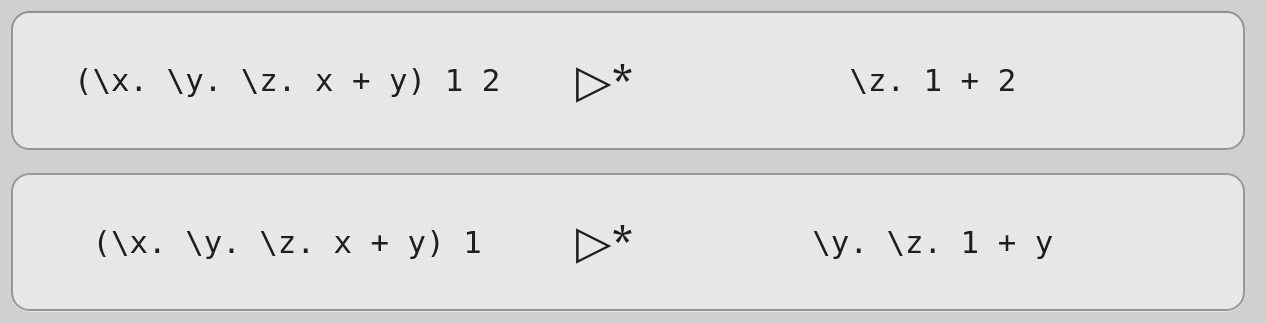
\includegraphics[width=0.75\linewidth]{images/conc_add.png}
\end{figure}

\noindent The first option is two reductions, the first of which is the second one. This relationship is not clear. This was discussed in the advanced focus group~\ref{ref:afg}, but development of a fix for this was not prioritized. 

\subsection{The Expressions Balloon During Evaluation}
\label{conc:baboon}
I believe that the languages lack of inbuilts is one of the languages best `features'. However, it is also a curse. Because everything is defined with match expressions, the expression balloons vertically with match statements during evaluation. For instance, in the provided `square\_sum' example:

% \begin{figure}[h]
\begin{lstlisting}[language=SFL]
square :: Int -> Int
square x = x * x

// List of the square numbers from lower to upper
list_of_squares :: Int -> Int -> List Int
list_of_squares lower upper = map square $ range lower upper

main :: Int
main = sum $ list_of_squares 1 5
\end{lstlisting}
% \end{figure}

\noindent Despite their being no match expressions, the `main' expression balloons to 3 match statements deep within 6 lazy steps:

% \begin{figure}[h]
\begin{lstlisting}[language=SFL]
match (match (match (infiniteFrom 1) {
    | Nil -> Nil
    | Cons x xs -> if ((5 - 1) > 0) (Cons x (take ((5 - 1) - 1) xs)) Nil
}) {
    | Nil -> Nil
    | Cons x xs -> Cons (square x) (map square xs)
}) {
    | Nil -> 0
    | Cons x xs -> (\x. \acc. x + acc) x (foldr (\x. \acc. x + acc) 0 xs)
}
\end{lstlisting}
% \end{figure}

The outer one comes from `sum', the middle one comes from `map', and the inner one comes from `range', all prelude functions. Unfortunately, this is hard to avoid, as pattern matching is a key concept in functional programming languages. Furthermore, a conclusion of the intermediate focus group was that the explicit match syntax, where it was obvious where/how pattern matching was occurring, made understanding pattern matching much easier. Indeed, they agreed that they would have liked to have SFL to learn about pattern matching rather than Haskell (see \ref{eval:IFG}). 

This situation could be improved by being able to select which functions we are interested in seeing the expansion of, and which ones we are not. See \ref{fw:function_checkboxes}

% \subsection{There is No Documentation}
% When designing the new UI (\ref{c2:next_ui}), I included buttons that would create help menus, and more information about the project, as well as instructions. However, these are time-consuming to write,  and I did not have time. 

\section{Future Work}
\label{conc:future_work}
\paragraph{Add More Documentation to the Website} As the language is quite similar to Haskell, an advanced user would not have much trouble figuring out how the website works. This works fine for a lecture tool as the lecturer would be able to figure it out, but the lack of documentation is detrimental to other users. 
\paragraph{Other Evaluation Strategies}
Users could have the option to pick the evaluation strategy. They can manually pick the evaluation strategy using free choice mode, but a mode that enforces strict evaluation for example would be useful to have. 
\paragraph{Improve Free Choice Mode}
Inspiration could be taken from the UI used by \llessons~\ref{bg:llessons_ui} where the expression to be evaluated could be selected by clicking on the input text itself. 
\paragraph{Keyboard Controls} This was requested by Samantha, my client, in our final meeting~\ref{c4:client}. She requested keyboard controls to be able to step forward and backward using our chosen evaluation strategy. 
\paragraph{Step to the End Button} This feature was requested by Amos during the intermediate focus group~\ref{eval:IFG}. A button would be provided to skip evaluation to the end of the program. This is not as trivial as it sounds, as the program may not terminate, and therefore crash the user's browser in trying to compute the final state. This problem could be avoided if we had keyboard controls, where holding in a certain button would repeatedly evaluate via the chosen reduction strategy. 
\paragraph{Selective Skipping}
\label{fw:function_checkboxes}
We are not always interested in all the functions involved in our program. For instance, if a lecturer is attempting to demonstrate \verb|foldr| over a list, they may not be interested in the expansion of how \verb|range| works in order to generate their list they are going to fold over. They may want the evaluation of some things to be `skipped'. 

We could mark certain expressions as uninteresting, and evaluate them as much as we can immediately. For instance, if the syntax for an uninteresting expression looked like `[e]':

\begin{lstlisting}[language=SFL]
main :: Int 
main = sum $ [range 1 4]
\end{lstlisting}

\noindent We could fully evaluate `\lstinline[language=SFL]|range 1 4|' to `\lstinline[language=SFL]|Cons 1 (Cons 2 (Cons 3 Nil))|'. However, this could cause issues if the term does not evaluate. 

% \begin{lstlisting}[language=SFL]
% fix f = f $ fix f

% id x = x

% main = if true 1 [fix id]
% \end{lstlisting}

% The evaluation of `\lstinline[language=SFL]|fix id|' will never terminate. If we were to attempt to evaluate this, it would run forever. If we were to provide a mechanism that forces full evaluation of a term, we would be providing functionality that the user could use to `shoot themselves in the foot'. This would need to be clearly communicated to the user, and a mechanism of stopping this evaluation should be provided if the user judges it has been too long. 



\paragraph{Extensions to the language}
As suggested by Amos during the intermediate focus group (\ref{eval:IFG}) the language could be extended with typeclasses. 

\backmatter\bibliography{dissertation}
\appendix

\chapter{AI Usage}
\label{appx:ai_prompt}

I did not directly prompt any Large Language Models, or any other AI model, to assist with the writing of my dissertation or implementation. However, as listed in the Supporting Technologies list, I used GitHub Copilot to help with writing some tests for the parser and type checker. I used it via the VS Code extension, which uses the context of your file, to provide advanced AI autocompletion.

% =============================================================================

\chapter{Tokens for Lexical Analysis}
\label{appx:tokens}
Below is the code for how tokens outputted by lexical analysis are defined. 
\begin{lstlisting}
enum TokenType {
    EOF,
    Newline,

    Id,
    UppercaseId,

    If,
    Then,
    Else,

    Match,
    LBrace,
    RBrace,

    IntLit,
    FloatLit,
    StringLit,
    CharLit,
    BoolLit,

    DoubleColon,
    RArrow,
    Forall,
    KWType,
    KWData,

    LParen,
    RParen,

    Lambda,

    Dollar,
    Dot,
    Comma,
    Bar,

    Assignment,
}

struct Token {
    tt: TokenType,
    value: String,
}
\end{lstlisting}

\chapter{How the System Looked During Various Testing Stages}
\section{End of Cycle 1}
\begin{figure}[h]
    \centering
    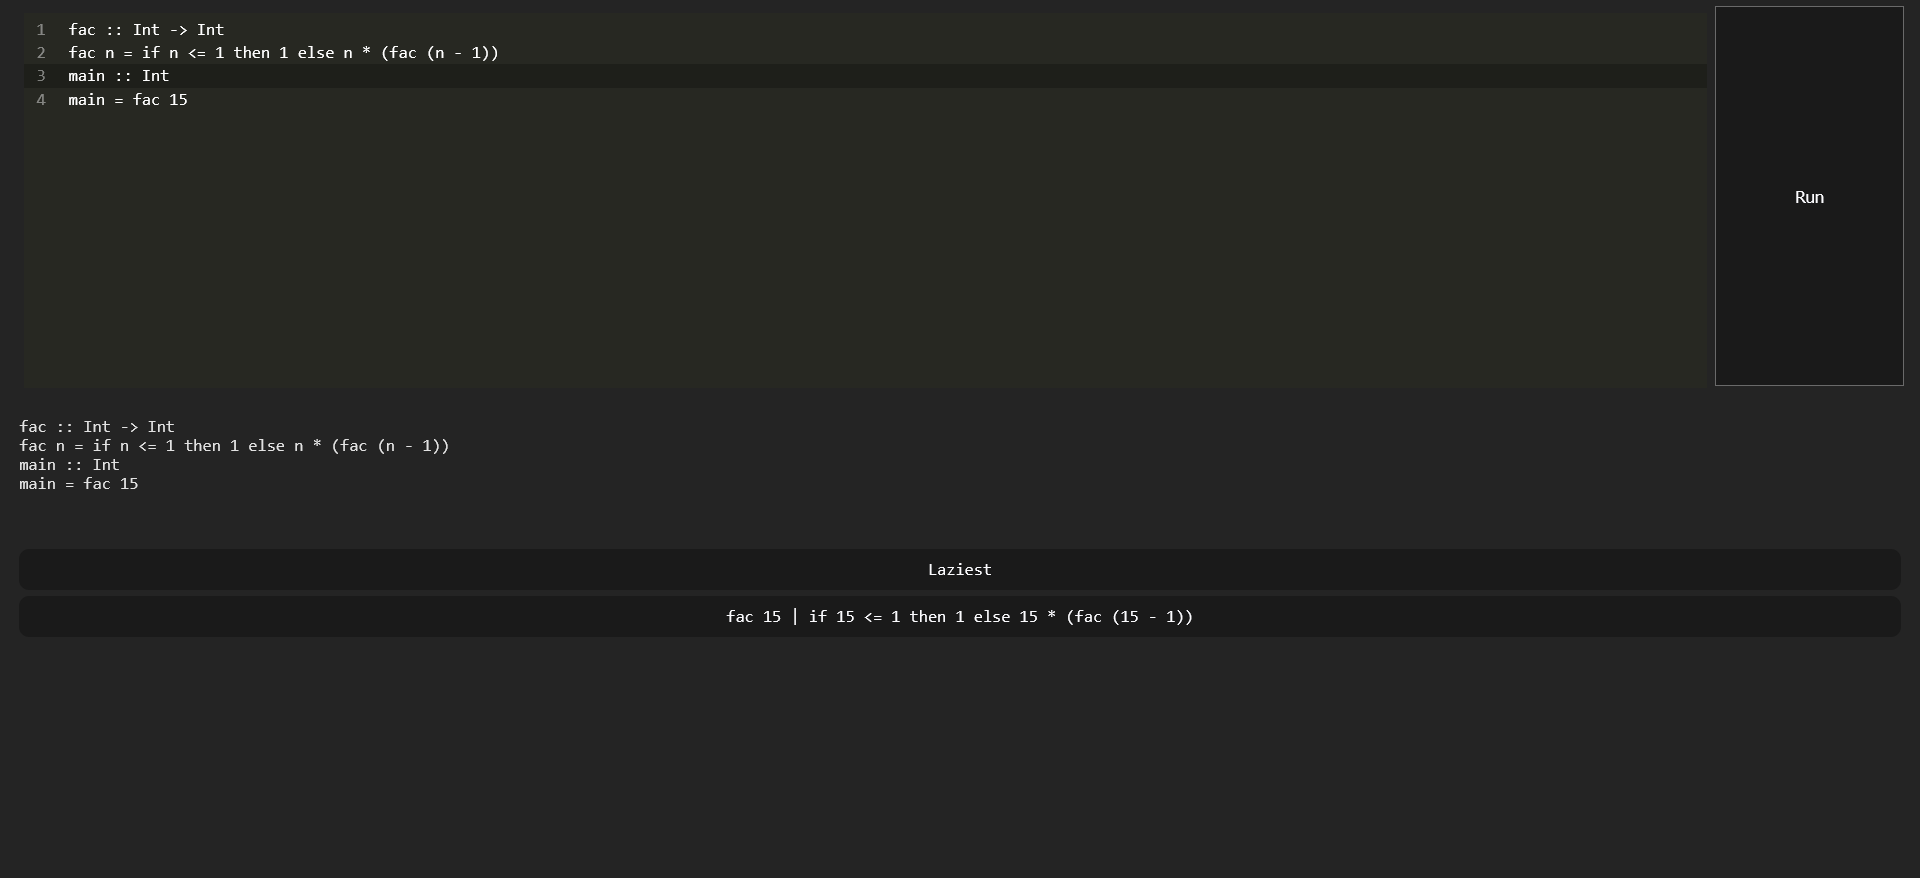
\includegraphics[width=1\linewidth]{images/cycle-1-end.png}
    \caption{The Web UI MVP, as presented to my client at the end of cycle 1. Note that this does have type assignments, but these were just ignored by the parser and typechecker at this stage. }
    \label{fig:screenshot_cycle_1_end}
\end{figure}
\section{Testathon}

\begin{figure}[h]
    \centering
    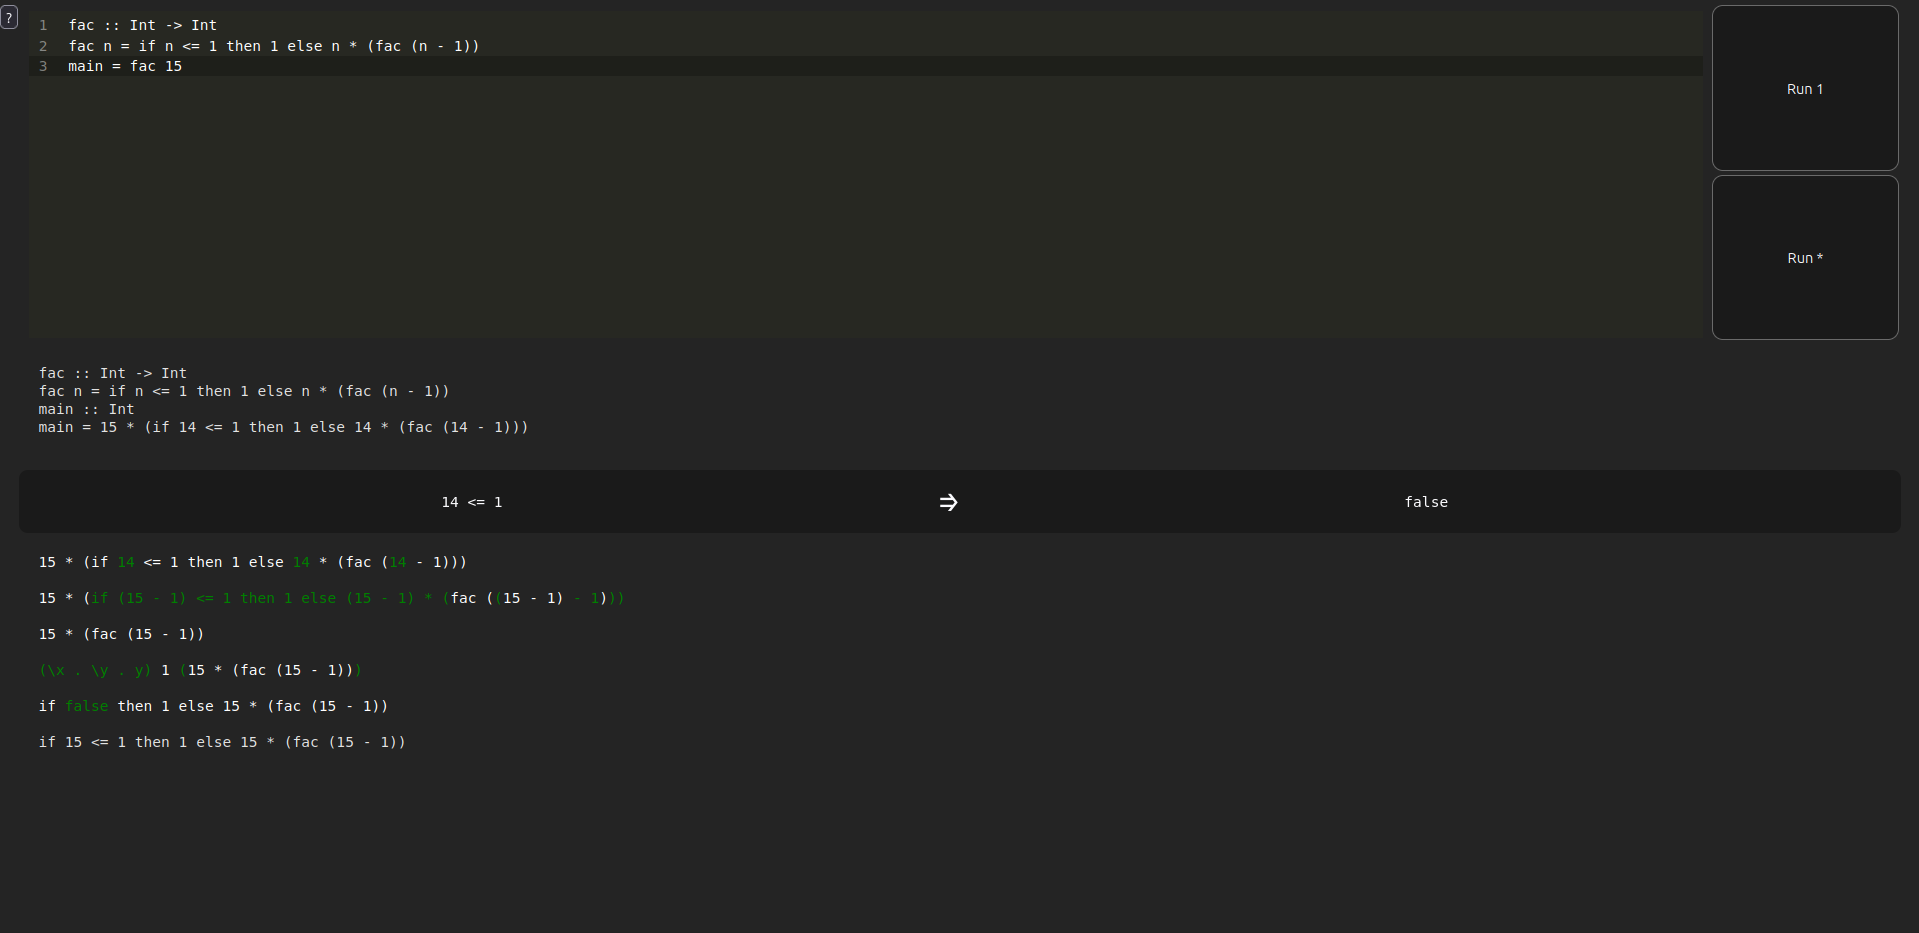
\includegraphics[width=1\linewidth]{images/product_at_testathon.png}
    \caption{The UI as tested in the testathon}
    \label{fig:screenshot_testathon}
\end{figure}

\begin{figure}
    \centering
    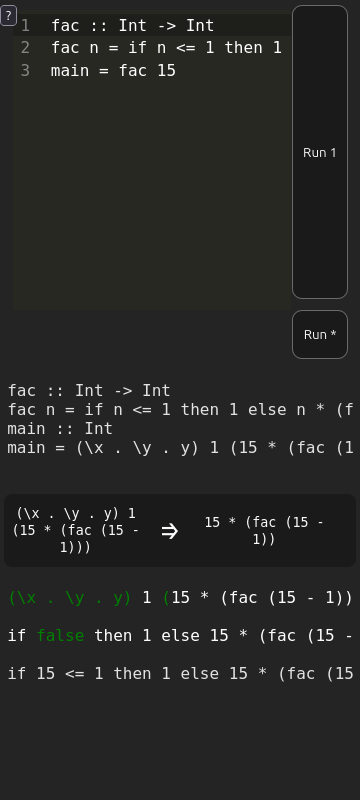
\includegraphics[width=0.5\linewidth]{images/testathon-mobile.png}
    \caption{The UI as tested in the testathon, as it would have appeared on a Samsung Galaxy S20}
    \label{fig:screenshot_testathon_mobile}
\end{figure}

\begin{figure}
    \centering
    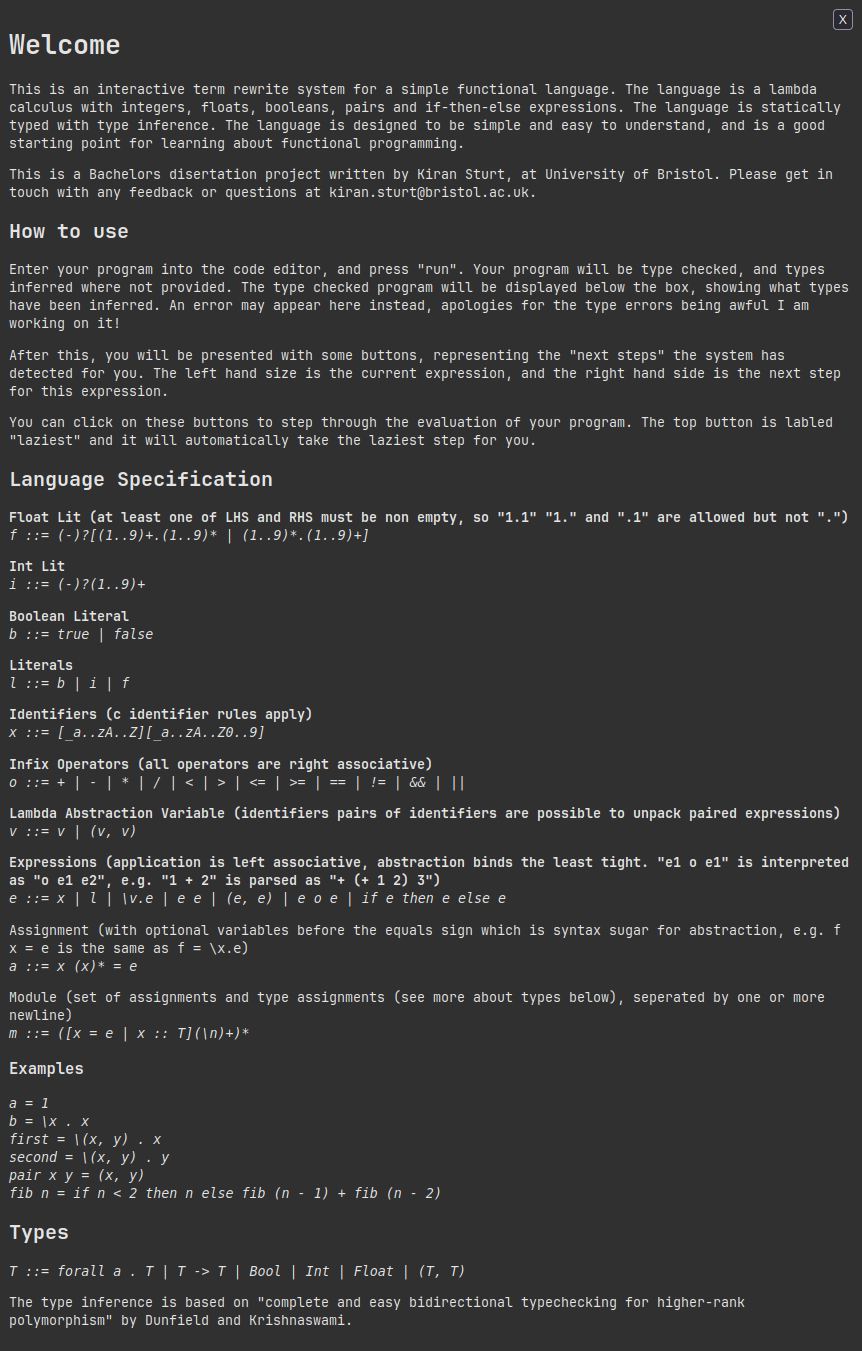
\includegraphics[width=0.9\linewidth]{images/testathon_help_menu_cropped.png}
    \caption{The "Help menu" in the testathon. This was spawned by pressing the "?" button in the top left of the UI, and dismissed by pressing the "X" button, or clicking outside of the box}
    \label{fig:screenshot_testathon_2}
\end{figure}

\chapter{Type System}
\def\OPTIONConf{1}
\linespread{1}

\renewcommand{\mathstrut}{\rule[-1pt]{0pt}{2pt}}

\def\OPTIONLoudLabels{0}
\def\OPTIONArxiv{1}

\definecolor{dHilite}{rgb}{0.9, 0.9, 0.6}
\definecolor{dRed}{rgb}{0.65, 0.0, 0.0}
\definecolor{dGreen}{rgb}{0.0, 0.65, 0.0}
\definecolor{dDkGreen}{rgb}{0.0, 0.35, 0.0}
\definecolor{dBlue}{rgb}{0.0, 0.0, 0.65}
\definecolor{dPurple}{rgb}{0.65, 0.0, 0.65}
\definecolor{dDigPurple}{rgb}{0.5, 0.0, 0.5}
\definecolor{dFaint}{rgb}{0.7, 0.7, 0.7}
\definecolor{dGray}{rgb}{0.5, 0.5, 0.5}
\definecolor{dDark}{rgb}{0.2, 0.2, 0.2}
\definecolor{dAlmostBlack}{rgb}{0.1, 0.1, 0.1}

\makeatletter
\def\url@MGstyle{%
\def\UrlFont{\tiny\huge\ttfamily}%
%
%
\Url@do
}
\makeatother
%
%
\newcommand{\marginPseudoURL}[1]{\tt #1}
\newcommand{\marginnote}[1]{\marginparwidth=40pt \marginpar{%
    \raisebox{-2ex}{\parbox{40pt}{\raggedright\scriptsize #1}}}}

\makeatletter
\def\url@vttstyle{%
  \@ifundefined{selectfont}{\def\UrlFont{\tt}}{\def\UrlFont{\normalfont\fontfamily{cmvtt}\selectfont}}}
\makeatother
%
\urlstyle{vtt}

%
%
%
%
%
%

\newcommand\textvtt[1]{{\normalfont\fontfamily{cmvtt}\selectfont #1}}

\newcommand{\LoudLabel}[1]{\idempotentlabel{#1}%
\ifnum\OPTIONLoudLabels=1%
  \ifnum\OPTIONConf=1%
  \marginnote{\tiny\textvtt{#1}}%
  \else%
  \marginnote{\textvtt{#1}}%
  \fi%
\fi%
}

\newcommand{\idempotentlabel}[1]{%
    \ifcsname IDEMPFLAG#1\endcsname%
      %
      \message{YYY ALREADY DEFINED: #1}
    \else%
      %
      \message{YYZ NOT ALREADY DEFINED: #1}
      \expandafter\gdef\csname IDEMPFLAG#1\endcsname{d}%
      %
      \label{#1}%
    \fi}

%

%
\ifnum\OPTIONLoudLabels=1%
\newcommand{\Label}[1]{\LoudLabel{#1}}%
\newcommand{\FLabel}[1]{\idempotentlabel{#1}%
{\tt\scriptsize{#1}}}%
\else%
\newcommand{\Label}[1]{\idempotentlabel{#1}}%
\newcommand{\FLabel}[1]{\idempotentlabel{#1}}%
\fi

%
%
%
%
%
%
%
%
\newdimen\zzfontsz
\newcommand{\fontsz}[2]{\zzfontsz=#1%
{\fontsize{\zzfontsz}{1.2\zzfontsz}\selectfont{#2}}}

\newcommand{\texfontsz}[1]{\zzfontsz=#1%
\fontsize{\zzfontsz}{1.25\zzfontsz}\selectfont}

\newcommand{\mathsz}[2]{\text{\fontsz{#1}{$#2$}}}

\newcommand{\XX}{\text{\ding{55}}}
\newcommand{\redXX}{\text{\textcolor{dRed}{\XX}}}
\newcommand{\greencheck}{\text{\textcolor{dGreen}{\checkmark}}}

\newcommand{\fixme}[1]{\textcolor{red}{\texttt{FIXME: {#1}}}}

\newcommand{\flaming}[1]{\textcolor{red}{\fontsz{18pt}{\bf #1}}}
\newcommand{\flamingmath}[1]{\textcolor{red}{\fontsz{18pt}{\bf \ensuremath{#1}}}}

\newcommand{\semiflaming}[1]{\textcolor{dRed}{\sl #1}}

% \newcommand{\mathcolor}[2]{\text{\textcolor{#1}{\ensuremath{#2}}}}

%
\newcommand{\smallblacktriangle}{\text{\textscale{0.7}{$\blacktriangleright$}}}

\newcommand{\setof}[1]{\left\{#1\right\}}
\newcommand{\comprehend}[2]{\setof{{#1} \;\middle|\; {#2}}}

\newcommand{\assign}{\ensuremath{\,{:=}\,}}

\newcommand{\arr}{\rightarrow}
%
%
\def\CompactJudgments{0}
\newcommand{\entails}{\mathrel{\ifnum\CompactJudgments=1%
    \vdash%
  \else%
     \vdash\,%
  \fi}}
\newcommand{\ctxoutsym}{\ifnum\CompactJudgments=1%
    \dashv%
  \else%
     \,\dashv%
  \fi}
\newcommand{\ctxout}[1]{\mathrel{\ctxoutsym}{#1}}

%
\newcommand{\J}{\mathcal{J}}
\newcommand{\judg}{\J}

\newcommand{\MonnierCommaSym}{{\smallblacktriangle}}
\newcommand{\MonnierComma}[1]{{\MonnierCommaSym}_{#1}}

\newcommand{\FV}[1]{\mathrm{FV}(#1)}
\newcommand{\xfev}{\mathsf{FEV}}
\newcommand{\fev}[1]{\xfev(#1)}
\newcommand{\FEV}[1]{\fev{#1}}
\newcommand{\xfsolev}{\mathsf{FSolEV}}
\newcommand{\fsolev}[2]{\xfsolev_{#1}(#2)}

\newcommand{\beeq}{=_{\beta\eta}}

\newcommand{\kindstar}{\star}
\newcommand{\kindnat}{\mathbb{N}}

\newcommand{\inversefn}[1]{{#1}^{-1}}

\newcommand{\emptysig}{\cdot}
\newcommand{\emptyctx}{\cdot}

\newcommand{\natzero}{\mathsf{zero}}
\newcommand{\xnatsucc}{\mathsf{succ}}
\newcommand{\natsucc}[1]{\xnatsucc\texttt{(}{#1}\texttt{)}}


\newcommand{\instantiate}[1]{{#1}\texttt{[-]}}
\newcommand{\quantify}[1]{\Lambda{#1}.\,}


\newcommand{\exvar}[1]{\widehat{#1}}
\newcommand{\exalpha}{\exvar{\alpha}}
\newcommand{\exbeta}{\exvar{\beta}}

\newcommand{\alln}[1]{\forall{#1}{:}\kindnat.\,}

\newcommand{\Match}[2]{{#1} \Rightarrow {#2}}
\newcommand{\matchor}{\ensuremath{\normalfont\,\texttt{|}\hspace{-5.35pt}\texttt{|}\,}}
\newcommand{\ind}[3]{\mathsf{ind}\texttt{(}\Match{\natzero}{#1}%
                     \texttt{,\;}%
                     \Match{\natsucc{#2}}{#3}
                     \texttt{)}}

\newcommand{\exunk}[2]{{#1} : {#2}}
\newcommand{\exsol}[3]{{#1} : {#2} \texttt{=} {#3}}
\newcommand{\exsolnokind}[2]{{#1} \texttt{=} {#2}}
\newcommand{\exsolwild}[2]{({#1} : {#2}\dots)}
\newcommand{\rexvar}[2]{\exsolnokind{#1}{#2}}

\newcommand{\tyname}[1]{\textsf{\normalfont #1}}
%
\newcommand{\unitexp}{\text{\normalfont \tt()}}
\newcommand{\unitty}{\tyname{1}}

\newcommand{\trientails}{\mathrel{{\rhd}\,}}
\newcommand{\trictxoutsym}{{\lhd}}
\newcommand{\trictxout}[1]{\mathrel{\trictxoutsym}{#1}}

\newcommand{\subtypingycolor}[1]{\textcolor{dDigPurple}{#1}}
%
\newcommand{\subtype}{\mathrel{\normalfont\texttt{\subtypingycolor{<:}}}}  %
\newcommand{\declsubtype}{\mathrel{\leq}}

\newcommand{\etal}{{et al.}}
\newcommand{\eg}{e.g.\ }
\newcommand{\ie}{i.e.\ }
\newcommand{\ala}{\`a la\ }
\newcommand{\Wlog}{w.l.o.g.\ }
\newcommand{\visavis}{vis-\`a-vis\ }
\newcommand{\Ocaml}{{OCaml}\xspace}
\newcommand{\OCaml}{\Ocaml}

\newcommand{\naive}{na\"ive\xspace}
\newcommand{\Backslash}{\char"5C}
\newcommand{\Lbrack}{\char"5B}
\newcommand{\Rbrack}{\char"5D}
\newcommand{\Lbrace}{\char"7B}
\newcommand{\Rbrace}{\char"7D}

\newcommand{\Appendixref}[1]{Appendix \ref{#1}}
\newcommand{\Figureref}[1]{Figure \ref{#1}}
\newcommand{\Figref}[1]{Fig.\ \ref{#1}}
\newcommand{\Sectionref}[1]{Section \ref{#1}}
\newcommand{\Secref}[1]{Sec.\ \ref{#1}}
\newcommand{\Chapterref}[1]{Chapter \ref{#1}}

\newcommand{\Listingref}[1]{Listing \ref{#1}}

\newcommand{\Theoremref}[1]{Theorem \ref{#1}}
\newcommand{\Thmref}[1]{Thm.\ \ref{#1}}
\newcommand{\Corollaryref}[1]{Corollary \ref{#1}}
\newcommand{\Corref}[1]{Cor.\ \ref{#1}}
\newcommand{\Lemmaref}[1]{Lemma \ref{#1} (\nameref{#1})}   %
\newcommand{\Lemref}[1]{\Lemma \ref{#1}}   %
%
\newcommand{\Conjectureref}[1]{Conjecture \ref{#1}}
\newcommand{\Propositionref}[1]{Proposition \ref{#1}}
\newcommand{\Propertyref}[1]{Property \ref{#1}}
\newcommand{\Remarkref}[1]{Remark \ref{#1}}
\newcommand{\Tableref}[1]{Table \ref{#1}}

\newcommand{\Definitionref}[1]{Definition \ref{#1}}
\newcommand{\Defnref}[1]{Def.\ \ref{#1}}

%
\newcommand{\ProofCaseRule}[1]{\item \textbf{Case }\textrm{{#1}}: ~ }
\newcommand{\ProofCaseThing}[1]{\ProofCaseRule{\ensuremath{#1}}}
\newcommand{\ProofCasesRules}[1]{\item \textbf{Cases }\textrm{{#1}}: ~ }
\newcommand{\ProofCaseRuleNoColon}[1]{\item \textbf{Case }\textrm{{#1}}}

\gdef\xxDerivationProofCaseColor{N}
\newcommand{\Begincolorcases}[1]{\gdef\xxDerivationProofCaseColor{#1}}
\newcommand{\Endcolorcases}{\gdef\xxDerivationProofCaseColor{N}}

%
%
%
%
%
%
%
%
%
%
%
%
%
%
%
%
%
%
%
%
%
%
%
\newcommand{\DerivationProofCase}[3]{%
     \smallskip
     \item %
       \parbox[t]{100ex}{%
       \textbf{Case } \\[-0.5em]
       $~$\hspace{5ex}
       \if\xxDerivationProofCaseColor N%
           \ensuremath{%
              \Infer{#1}{#2}{#3}%
            }
       \else%
           \colorbox{\xxDerivationProofCaseColor}{%
              \ensuremath{%
                \Infer{#1}{#2}{#3}%
              }%
           }%
        \fi%
     }%
     \nopagebreak \\[-0.8ex]
  }

\newcommand{\DoubleDerivationProofCase}[6]{%
     \smallskip
     \item %
       \parbox[t]{100ex}{%
       \textbf{Case } \\[-0.5em]
       $~$\hspace{5ex}
       \if\xxDerivationProofCaseColor N%
           \ensuremath{%
              \Infer{#1}{#2}{#3}%
              ~~~~~
              \Infer{#4}{#5}{#6}%
            }
       \else%
           \colorbox{\xxDerivationProofCaseColor}{%
              \ensuremath{%
                \Infer{#1}{#2}{#3}%
                ~~~~~
                \Infer{#4}{#5}{#6}%
              }%
           }%
        \fi%
     }%
     \nopagebreak \\[-0.8ex]
  }

\newcommand{\Dee}{\mathcal{D}}
\newcommand{\D}{\mathcal{\Dee}}

\newenvironment{displ}{\vspace{1pt} \begin{center} ~\!\!}{\end{center}}
\newenvironment{mathdispl}{\vspace{1pt} \begin{center} ~\!\!\(}{\)\end{center}}

\newenvironment{ctabular}{%
      \renewcommand{\arraystretch}{1}%
         \vspace{1pt}%
         \begin{center} ~\!\!%
           \begin{tabular}[t]{l}%
     }{%
            \end{tabular}%
          \end{center}%
      }

\newcommand{\arrayenv}[1]{\renewcommand{\arraystretch}{1} \begin{array}[t]{@{}c@{}}#1\end{array}}
\newcommand{\arrayenvc}[1]{\renewcommand{\arraystretch}{1} \begin{array}[c]{@{}c@{}}#1\end{array}}
\newcommand{\arrayenvcl}[1]{\renewcommand{\arraystretch}{1} \begin{array}[c]{@{}l@{}}#1\end{array}}
\newcommand{\arrayenvr}[1]{\renewcommand{\arraystretch}{1} \begin{array}[t]{@{}r@{}}#1\end{array}}
\newcommand{\arrayenvbr}[1]{\renewcommand{\arraystretch}{1} \begin{array}[b]{@{}r@{}}#1\end{array}}
\newcommand{\arrayenvl}[1]{\renewcommand{\arraystretch}{1} \begin{array}[t]{@{}l@{}}#1\end{array}}
\newcommand{\arrayenvb}[1]{\renewcommand{\arraystretch}{1}  \begin{array}[b]{@{}c@{}}#1\end{array}} 
\newcommand{\arrayenvbl}[1]{\renewcommand{\arraystretch}{1}  \begin{array}[b]{@{}l@{}}#1\end{array}}
\newcommand{\arrayenvblll}[1]{\renewcommand{\arraystretch}{1}  \begin{array}[b]{@{}lll@{}}#1\end{array}}
\newcommand{\pfarr}[1]{\begin{array}[b]{@{}l@{}}#1\end{array}}

%
\newcommand{\BeginProof}{\renewcommand{\arraystretch}{1.1} \begin{tabular}[b]{r@{}r @{} l  l}}
\newcommand{\EndProof}{\end{tabular} \renewcommand{\arraystretch}{\mydefaultarraystretch}}

\newcommand{\Hand}{\text{\Pointinghand~~~~}}

\newcommand{\Pf}[4] {&$#1$ $#2$\, & $#3$ & #4 \\}
\newcommand{\Pfmrg}[3] {&$#1$\, & $#2$ & #3 \\}
\newcommand{\stepPf}[3] {\Pf{#1}{\,\step\,}{#2}{#3}}
\newcommand{\EPf}[3] {\Pf{#1}{\Entails}{#2}{#3}}
\newcommand{\LetPf}[3] {\Pf{\text{Let}\,~{#1}}{=\,}{#2\text{.}}{#3}}
\newcommand{\ForallPf}[3] {\Pf{\text{For all}\,~{#1}}{\in\,}{#2}{#3}}
\newcommand{\mkpf}[4] {\Pf{#2}{#1\,}{#3}{#4}}

\newcommand{\ePf}[3] {\mkpf{\entails}{#1}{#2}{#3}}
\newcommand{\eqPf}[3] {\mkpf{=}{#1}{#2}{#3}}
\newcommand{\continueeqPf}[2] {\mkpf{=}{~}{#1}{#2}}
\newcommand{\rightstarteqPf}[1] {\mkpf{~}{~}{#1}{~}}
\newcommand{\neqPf}[3] {\mkpf{\neq}{#1}{#2}{#3}}
\newcommand{\ltPf}[3] {\mkpf{<}{#1}{#2}{#3}}
\newcommand{\leqPf}[3] {\mkpf{\leq}{#1}{#2}{#3}}
\newcommand{\inPf}[3] {\mkpf{\in}{#1}{#2}{#3}}
\newcommand{\notinPf}[3] {\mkpf{\notin}{#1}{#2}{#3}}

\newcommand{\trailingjust}[1]{\Pf{}{}{}{~~{#1}}}
\newcommand{\derivesPf}[1]{${#1} \derives~~$}

\newcommand{\contraPf}[1] {%
          \Pf{\Rightarrow\Leftarrow}{}{} {}%
          \Pf{#1}{}{} {By contradiction}%
       }

\newcommand{\NOTePf}[3] {\Pf{#1}{\not\entails\;}{#2}{#3}}
\newcommand{\proofsep}{\,\\[-0.5em]}
\newcommand{\PfTwo}[7]{\Pf{\arrayenvr{{#1}\\{#4}}}{\arrayenvl{{#2}\\{#5}}}{\arrayenvl{{#3}\\{#6}}}%
                                              {\drophalf{\!\ensuremath{\left\} \begin{array}{r l} \,\\ \, \end{array}\!\!\!\!\!%
                                                      \text{#7} \right.}}}}
\newenvironment{llproof}{\BeginProof}{\EndProof}
\newcommand{\decolumnizePf}{\end{llproof} ~\\ \begin{llproof}}

%
\newcommand{\proofheading}[1]{}  %

\newcommand{\ditto}{\ensuremath{''}}


\newcommand{\xdom}{\mathsf{dom}}
\newcommand{\dom}[1]{\xdom(#1)}

\newcommand{\xweight}{\mathsf{weight}}
\newcommand{\weight}[2]{\xweight_{#1}(#2)}

\newcommand{\xangst}{\mathsf{angst}}
\newcommand{\angst}[2]{\xangst_{#1}(#2)}

\newcommand{\xunsol}{\mathsf{unsol}}
\newcommand{\unsol}[2]{\xunsol_{#1}(#2)}

\newcommand{\xunsolved}{\mathsf{unsolved}}
\newcommand{\unsolved}[1]{\xunsolved(#1)}

\newcommand{\xGtypesize}[1]{\mathsf{size}_{#1}}
\newcommand{\Gtypesize}[2]{\xGtypesize{#1}(#2)}

\newcommand{\union}{\mathrel{\cup}}
\newcommand{\sect}{\mathrel{\cap}}


\newcommand{\normalize}{\mathrel{\Downarrow}}


%
%
\newcommand{\textgraybox}[1]{\boxed{#1}}
\newcommand{\graybox}[1]{\textgraybox{\ensuremath{#1}}}

\newcommand{\tightcolorbox}[2]{\setlength{\fboxsep}{1pt}\colorbox{#1}{#2}}

%
\newcommand{\textcolorbox}[2]{\tightcolorbox{#1}{#2}}
\newcommand{\textshadebox}[1]{\textcolorbox{grayboxgray}{#1}}
%
\newcommand{\shadebox}[1]{\text{\textshadebox{\ensuremath{#1}}}}

%

%
\newcommand{\mathcolorbox}[2]{\text{\tightcolorbox{#1}{$\displaystyle {#2}$}}}

%
%
%
%

\newcommand{\judgboxfontsize}[1]{%
    \ifnum\OPTIONConf=1%
        \mathsz{11pt}{#1}%
    \else%
        \mathsz{14pt}{#1}%
    \fi}
\newcommand{\judgbox}[2]{%
      {\raggedright \textgraybox{\ensuremath{\judgboxfontsize{#1}}}\!%
        \fontsz{9pt}{\begin{tabular}[c]{l} #2 \end{tabular}} %
}}


\newcommand{\bnfas}{\mathrel{::=}}
\newcommand{\bnfalt}{\mathrel{\mid}}

\newcommand{\derives}{\mathrel{::}}

\newcommand{\AllSym}{\forall}
\newcommand{\xAll}[1]{\AllSym#1}
\newcommand{\All}[1]{\xAll{#1}.\:}

\newcommand{\AND}{\text{~~and~~}}

\newcommand{\Infer}[3]{\inferrule*[right={\text{\strut#1}}]{{}#2\mathstrut}{{}#3\mathstrut}}




\newcommand{\keyword}[1]{\textsf{#1}}
\newcommand{\textkw}[1]{\keyword{#1}}
\newcommand{\lam}[1]{\lambda #1.\,}
\newcommand{\fun}[2]{\lam{#1}{#2}}
\newcommand{\typelam}[1]{\Lambda #1.\,}
\newcommand{\LAM}[1]{\typelam{#1}}
\newcommand{\Let}[2]{\textkw{let}\;{#1}\,\texttt{=}\,{#2}\;\textkw{in}\;}

\newcommand{\bigprec}{\mathrel{\mathsz{14pt}{\prec}}}


\newcommand{\atomic}[1]{{#1}\;\mathrm{atomic}}

\newcommand{\declsubjudg}[3]{\ensuremath{{#1} \entails {#2} \declsubtype {#3}}}
\newcommand{\typejudg}[3]{\ensuremath{{#1} \entails {#2} : {#3}}}
\newcommand{\subjudg}[4]{\ensuremath{{#1} \entails {#2} \subtype {#3} \ctxout{#4}}}

%
%
\newdimen\zzinstsymLTwidth
\newdimen\zzinstsymEQwidth
\newdimen\zzinstsymDiff
\newcommand{\instsymLeq}{%
    \settowidth{\zzinstsymLTwidth}{\text{\normalfont\tt<}}%
    \settowidth{\zzinstsymEQwidth}{\text{\normalfont=}}%
    \setlength{\zzinstsymDiff}{\zzinstsymEQwidth}%
    \addtolength{\zzinstsymDiff}{-\zzinstsymLTwidth}%
    \text{\raisebox{-0.22ex}{\normalfont=}%
%
    \hspace{-\zzinstsymEQwidth}%
    \hspace{0.5\zzinstsymDiff}%
    \raisebox{0.77ex}{\normalfont\tt<}}}
\newcommand{\instsymColon}{%
     \raisebox{-0.09ex}{\text{\normalfont{:}}}}
%
%
%
\newcommand{\instsyml}{\subtypingycolor{\instsymColon\hspace{0.05ex}\instsymLeq}}
\newcommand{\instsymr}{\subtypingycolor{\instsymLeq\hspace{0.05ex}\instsymColon}}
\newcommand{\instsymlop}{\mathrel{\instsyml}}
\newcommand{\instsymrop}{\mathrel{\instsymr}}

\newcommand{\instjudg}[4]{\ensuremath{{#1} \entails {#2} \instsymlop {#3} \ctxout{#4}}}
\newcommand{\instjudgr}[4]{\ensuremath{{#1} \entails {#3} \instsymrop {#2} \ctxout{#4}}}

\newcommand{\declsubjudgPf}[4] {\Pf{#1}{\entails}{{#2} \declsubtype {#3}}{#4}}
\newcommand{\subjudgPf}[5] {\Pf{#1}{\entails}{{#2} \subtype {#3} \ctxout{#4}}{#5}}
\newcommand{\substextendPf}[3] {\Pfmrg{{#1} \extendssym\,}{#2}{#3}}
\newcommand{\instjudgPf}[5]{\Pf{#1}{\entails}{{#2} {\;\instsyml\;} {#3} \ctxout{#4}}{#5}}
\newcommand{\instjudgrPf}[5]{\Pf{#1}{\entails}{{#3} {\;\instsymr\;} {#2} \ctxout{#4}}{#5}}

\newcommand{\chkcolor}{dBlue}
\newcommand{\syncolor}{dRed}
\newcommand{\appcolor}{dDkGreen}
\newcommand{\chk}{\mathrel{\mathcolor{\chkcolor}{\Leftarrow}}}
\newcommand{\uncoloredsyn}{{\Rightarrow}}
\newcommand{\syn}{\mathrel{\mathcolor{\syncolor}{\uncoloredsyn}}}
\newcommand{\appsep}{\;{\mathcolor{\appcolor}{\bullet}}\;}
%
\newcommand{\app}{\mathrel{\mathcolor{\appcolor}{{\uncoloredsyn}\hspace{-1.2ex}{\uncoloredsyn}}}}

\newcommand{\chkjudg}[4]{\ensuremath{{#1} \entails {#2} \chk {#3} \ctxout{#4}}}
\newcommand{\appjudg}[5]{\ensuremath{{#1} \entails {#3} \appsep {#2} \app {#4} \ctxout{#5}}}
\newcommand{\synjudg}[4]{\ensuremath{{#1} \entails {#2} \syn {#3} \ctxout{#4}}}

\newcommand{\declchkjudg}[3]{\ensuremath{{#1} \entails {#2} \chk {#3}}}
\newcommand{\declappjudg}[4]{\ensuremath{#1} \entails {#3} \appsep {#2}  \app {#4}}
\newcommand{\declsynjudg}[3]{\ensuremath{{#1} \entails {#2} \syn {#3}}}

\newcommand{\chkjudgPf}[5]{\Pf{#1}{\entails}{{#2} \chk {#3} \ctxout{#4}}{#5}}
\newcommand{\appjudgPf}[6]{\Pf{#1}{\entails}{{#3} \appsep {#2} \app {#4} \ctxout{#5}}{#6}}
\newcommand{\synjudgPf}[5]{\Pf{#1}{\entails}{{#2} \syn {#3} \ctxout{#4}}{#5}}
\newcommand{\declchkjudgPf}[4]{\Pf{#1}{\entails}{{#2} \chk {#3}}{#4}}
\newcommand{\declappjudgPf}[5]{\Pf{#1}{\entails}{{#3} \appsep {#2} \app {#4}}{#5}}
\newcommand{\declsynjudgPf}[4]{\Pf{#1}{\entails}{{#2} \syn {#3}}{#4}}


\newcommand{\hyp}[2]{{#1}:{#2}}
\newcommand{\hypeq}[2]{{#1} = {#2}}
\newcommand{\tighthypeq}[2]{{#1}{=}{#2}}
%
\newcommand{\alltype}[1]{\All{#1}}
\newcommand{\num}{\mathsf{int}}
\newcommand{\bool}{\mathsf{bool}}

\newcommand{\grow}[2]{{#1} \sqsupseteq {#2}}

\newcommand{\idsubst}{\mathsf{id}}

\newcommand{\extendssym}{\longrightarrow}
\newcommand{\extends}[2]{{#1} \extendssym {#2}}
%
\newcommand{\substextend}[2]{\extends{#1}{#2}}

\newcommand{\judgetp}[2]{{#1} \entails {#2}}
\newcommand{\judgetpPf}[3]{\Pf{#1}{\entails}{#2}{#3}}
%
%
\newcommand{\typesize}[2]{|{#1} {\;\entails} {#2}|}

\newcommand{\judgectx}[1]{{#1}~\mathit{ctx}}
\newcommand{\judgectxPf}[2]{\Pf{}{}{\judgectx{#1}}{#2}}

\newcommand{\xcompletes}{\ensuremath{\mathsf{completes}}}
\newcommand{\xcompletedby}{\ensuremath{\mathsf{completed\;by}}}
%
\newcommand{\completedby}[2]{{#1} \;\flamingmath{\xcompletedby}\; {#2}}
\newcommand{\apply}[2]{{[{#1}]}{#2}}

\newcommand{\ahat}{\hat{\alpha}}
\newcommand{\bhat}{\hat{\beta}}
\newcommand{\chat}{\hat{\gamma}}
\newcommand{\dhat}{\hat{\delta}}

%
%
%
\newcommand{\hsubst}[5]{[{#2}/{#3}]^{#1}_{#2}{#4}}

%
%
%
\newcommand{\rulename}[1]{\text{\normalfont\textsf{#1}}}

%
%
%
\newcommand{\substextendrulename}[1]{\ensuremath{{\extendssym}{\rulename{#1}}}\xspace}
\newcommand{\substextendId}{\substextendrulename{ID}}

\newcommand{\substextendUU}{\substextendrulename{Uvar}}
\newcommand{\substextendVV}{\substextendrulename{Var}}
\newcommand{\substextendEE}{\substextendrulename{Unsolved}}
\newcommand{\substextendSolSol}{\substextendrulename{Solved}}
\newcommand{\substextendMonMon}{\substextendrulename{Marker}}

\newcommand{\substextendSolve}{\substextendrulename{Solve}}
\newcommand{\substextendAdd}{\substextendrulename{Add}}
\newcommand{\substextendAddSolved}{\substextendrulename{AddSolved}}


%
%
%
\newcommand{\Dsubrulename}[1]{\ensuremath{{\declsubtype}\rulename{#1}}\xspace}
\newcommand{\DsubVar}{\Dsubrulename{Var}}
\newcommand{\DsubUnit}{\Dsubrulename{Unit}}
\newcommand{\DsubArr}{\Dsubrulename{\ensuremath{\arr}}}
\newcommand{\DsubImp}{\DsubArr} %
\newcommand{\DsubAllL}{\Dsubrulename{\ensuremath{\forall}{L}}}
\newcommand{\DsubAllR}{\Dsubrulename{\ensuremath{\forall}{R}}}

%
%
%
\newcommand{\Subrulename}[1]{\ensuremath{{\subtype}\rulename{#1}}\xspace}
\newcommand{\SubVar}{\Subrulename{Var}}
\newcommand{\SubUnit}{\Subrulename{Unit}}
\newcommand{\SubExvar}{\Subrulename{Exvar}}
\newcommand{\SubArr}{\Subrulename{\ensuremath{\arr}}}
\newcommand{\SubImp}{\SubArr} %
\newcommand{\SubAllL}{\Subrulename{\ensuremath{\forall}{L}}}
\newcommand{\SubAllR}{\Subrulename{\ensuremath{\forall}{R}}}

\newcommand{\SubSubst}[1]{\Subrulename{\flaming{Subst{#1}}}}
\newcommand{\SubSubstL}{\SubSubst{L}}
\newcommand{\SubSubstR}{\SubSubst{R}}

\newcommand{\SubInst}[1]{\Subrulename{Instantiate{#1}}}
\newcommand{\SubInstL}{\SubInst{L}}
\newcommand{\SubInstR}{\SubInst{R}}

%
%
%
\newcommand{\DeclWFrulename}[1]{\ensuremath{\rulename{Decl{#1}WF}}\xspace}
\newcommand{\DeclUvarWF}{\DeclWFrulename{Uvar}}
\newcommand{\DeclUnitWF}{\DeclWFrulename{Unit}}
\newcommand{\DeclArrowWF}{\DeclWFrulename{Arrow}}
\newcommand{\DeclForallWF}{\DeclWFrulename{Forall}}

%
%
%
\newcommand{\WFrulename}[1]{\ensuremath{\rulename{{#1}WF}}\xspace}
\newcommand{\UvarWF}{\WFrulename{Uvar}}
\newcommand{\UnitWF}{\WFrulename{Unit}}
\newcommand{\EvarWF}{\WFrulename{Evar}}
\newcommand{\SolvedEvarWF}{\WFrulename{SolvedEvar}}
\newcommand{\ArrowWF}{\WFrulename{Arrow}}
\newcommand{\ForallWF}{\WFrulename{Forall}}


%
%
%
\newcommand{\CWFrulename}[1]{\ensuremath{\rulename{{#1}Ctx}}\xspace}
\newcommand{\EmptyCWF}{\CWFrulename{Empty}}
\newcommand{\UvarCWF}{\CWFrulename{Uvar}}
\newcommand{\EvarCWF}{\CWFrulename{Evar}}
\newcommand{\SolvedEvarCWF}{\CWFrulename{SolvedEvar}}
\newcommand{\VarCWF}{\CWFrulename{Var}}
\newcommand{\MarkerCWF}{\CWFrulename{Marker}}


%
%
%
\newcommand{\Instrulename}[1]{\ensuremath{\rulename{Inst{#1}}}\xspace}
\newcommand{\InstLrulename}[1]{\Instrulename{L{#1}}}
\newcommand{\InstRrulename}[1]{\Instrulename{R{#1}}}

\newcommand{\InstLSolve}{\InstLrulename{Solve}}
\newcommand{\InstLReach}{\InstLrulename{Reach}}
\newcommand{\InstLArr}{\InstLrulename{Arr}}
\newcommand{\InstLAllR}{\InstLrulename{AllR}}

\newcommand{\InstRSolve}{\InstRrulename{Solve}}
\newcommand{\InstRReach}{\InstRrulename{Reach}}
\newcommand{\InstRArr}{\InstRrulename{Arr}}
\newcommand{\InstRAllL}{\InstRrulename{AllL}}


%
%
%
\newcommand{\CompletesRule}{\rulename{completes}}
%
%
%
%
%
%
%
%




%
%
%
\newcommand{\Decltyrulename}[1]{\ensuremath{\rulename{Decl#1}}\xspace}

\newcommand{\DeclIntrorulename}[1]{\Decltyrulename{\ensuremath{#1}I}}
\newcommand{\DeclIntroSynrulename}[1]{\Decltyrulename{\ensuremath{#1}I$\syn$}}
\newcommand{\DeclElimrulename}[1]{\Decltyrulename{\ensuremath{#1}E}}
\newcommand{\DeclApprulename}[1]{\Decltyrulename{\ensuremath{#1}App}}

%
\newcommand{\DeclVar}{\Decltyrulename{Var}}
\newcommand{\DeclSub}{\Decltyrulename{Sub}}
\newcommand{\DeclAnno}{\Decltyrulename{Anno}}

%
\newcommand{\DeclUnitIntro}{\DeclIntrorulename{\unitty}}
%
\newcommand{\DeclUnitIntroSyn}{\DeclIntroSynrulename{\unitty}}

%
\newcommand{\DeclArrIntro}{\DeclIntrorulename{\arr}}
\newcommand{\DeclArrIntroSyn}{\DeclIntroSynrulename{\arr}}
\newcommand{\DeclArrElim}{\DeclElimrulename{\arr}}

%
\newcommand{\DeclAllIntro}{\DeclIntrorulename{\AllSym}}
%
\newcommand{\DeclAllElim}{\DeclElimrulename{\AllSym}}

\newcommand{\DeclArrApp}{\DeclApprulename{\arr}}
%
\newcommand{\DeclAllApp}{\DeclApprulename{\forall}}
%

%
%
%
\newcommand{\Tyrulename}[1]{\ensuremath{\rulename{#1}}\xspace}

\newcommand{\Introrulename}[1]{\Tyrulename{\ensuremath{#1}I}}
\newcommand{\IntroSynrulename}[1]{\Tyrulename{\ensuremath{#1}I$\syn$}}
\newcommand{\Elimrulename}[1]{\Tyrulename{\ensuremath{#1}E}}
\newcommand{\Apprulename}[1]{\Tyrulename{\ensuremath{#1}App}}

%
\newcommand{\Var}{\Tyrulename{Var}}
\newcommand{\Sub}{\Tyrulename{Sub}}
\newcommand{\Anno}{\Tyrulename{Anno}}

%
\newcommand{\SubstSyn}{\Tyrulename{Subst$\syn$}}
\newcommand{\SubstChk}{\Tyrulename{Subst$\chk$}}

%
\newcommand{\UnitIntro}{\Introrulename{\unitty}}
%
\newcommand{\UnitIntroSyn}{\IntroSynrulename{\unitty}}

%
\newcommand{\ArrIntro}{\Introrulename{\arr}}
\newcommand{\ArrIntroSyn}{\IntroSynrulename{\arr}}
\newcommand{\ArrElim}{\Elimrulename{\arr}}

%
\newcommand{\AllIntro}{\Introrulename{\AllSym}}
%
\newcommand{\AllElim}{\Elimrulename{\AllSym}}

%
\newcommand{\ArrApp}{\Apprulename{\arr}}
%
\newcommand{\AllApp}{\Apprulename{\forall}}
%
\newcommand{\SubstApp}{\Apprulename{\rulename{Subst}}}
%
\newcommand{\SolveApp}{\Apprulename{\ahat}}
%

%
%
%
\newcommand{\subtermofsym}{\preceq}
\newcommand{\subtermof}{\mathrel{\subtermofsym}}
\newcommand{\propersubtermofsym}{\prec}
\newcommand{\propersubtermof}{\mathrel{\propersubtermofsym}}
\newcommand{\subtermofPf}[3] {\mkpf{\subtermof}{#1}{#2}{#3}}
\newcommand{\propersubtermofPf}[3] {\mkpf{\propersubtermof}{#1}{#2}{#3}}
\newcommand{\notsubtermofPf}[3] {\mkpf{\not\subtermof}{#1}{#2}{#3}}
\newcommand{\notpropersubtermofPf}[3] {\mkpf{\not\propersubtermof}{#1}{#2}{#3}}

\newcommand{\occursinsidearrow}{{\hspace{0.6ex}\raisebox{-0.4ex}{%
       \ensuremath{\propersubtermof\rput[b](-1.35ex,1.2ex){\ensuremath{\mathsz{1.4ex}{\arr}}}}}}}
\newcommand{\notoccursinsidearrow}{{\hspace{0.6ex}\raisebox{-0.4ex}{%
       \ensuremath{\propersubtermof{\rput[b](-2.3ex,0.0ex){\ensuremath{\not}}}\rput[b](-1.35ex,1.2ex){\ensuremath{\mathsz{1.4ex}{\arr}}}}}}}

\newcommand{\occursinsidearrowPf}[3] {\mkpf{\!\occursinsidearrow\!}{#1}{#2}{#3}}
\newcommand{\notoccursinsidearrowPf}[3] {\mkpf{\!\notoccursinsidearrow\!}{#1}{#2}{#3}}


%
%
%
\newcommand{\Ctxsubrulename}[1]{\ensuremath{\rulename{CtxSub#1}}\xspace}
\newcommand{\CtxsubEmpty}{\Ctxsubrulename{Empty}}
\newcommand{\CtxsubUvar}{\Ctxsubrulename{Uvar}}
\newcommand{\CtxsubVar}{\Ctxsubrulename{Var}}

%
%
%
\newcommand{\AssignRuleName}[1]{\ensuremath{\rulename{A#1}}\xspace}
\newcommand{\AssignIntroName}[1]{\AssignRuleName{\ensuremath{#1}I}}
\newcommand{\AssignElimName}[1]{\AssignRuleName{\ensuremath{#1}E}}
\newcommand{\AssignVar}{\AssignRuleName{Var}}
\newcommand{\AssignUnit}{\AssignRuleName{Unit}}
\newcommand{\AssignArrIntro}{\AssignIntroName{\arr}}
\newcommand{\AssignArrElim}{\AssignElimName{\arr}}
\newcommand{\AssignAllIntro}{\AssignIntroName{\forall}}
\newcommand{\AssignAllElim}{\AssignElimName{\forall}}
\newcommand{\judge}[3]{{#1} \vdash {#2} : {#3}}

%
%
%
\newcommand{\citepSequentCalculus}{\citep{Gentzen35}}
\newcommand{\citetSequentCalculus}{\citet{Gentzen35}}
\newcommand{\citepSubformulaProperty}{\citep[p.\ 87]{Gentzen35}}
\newcommand{\citetSubformulaProperty}{\citet[p.\ 87]{Gentzen35}}


%
%
%
%
\newcommand{\Fsub}{\ensuremath{{\text{F}}_{\texttt{<:}}}\xspace}

%
\newcommand{\Csharp}{\ensuremath{\text{\textrm{C}}^\sharp}}

%
\newcommand{\MLF}{\ensuremath{\mathsf{ML}^\mathsf{F}}\xspace}


%
%
%
\newcommand{\contextappvar}[2]{{[{#1}]}^\dagger{#2}}
\newcommand{\contextapp}[2]{{[{#1}]{#2}}}

\newcommand{\soln}[1]{\left|{#1}\right|}    %

\newcommand{\equivctxsym}{\simeq}
\newcommand{\equivctx}[2]{{#1} \equivctxsym {#2}}

\newcommand{\LOCALCOPY}[1]{%
          \href{papers/#1}{\bf \textcolor{dGreen}{local copy}}}


\newcommand{\Uniontype}{$\bigcup$}
\newcommand{\Unionname}{\text{Name}}
\newcommand{\Producttype}{$\times$}

\newcommand{\TypeAlias}[2]{[#1 : #2]}

\newcommand{\Aliasrulename}{\Tyrulename{\ensuremath{}Alias}}
\newcommand{\Pairsynthrulename}{\Tyrulename{\Producttype$\syn$}}
\newcommand{\Intsynthrulename}{\Tyrulename{IntLit$\syn$}}
\newcommand{\Boolsynthrulename}{\Tyrulename{BoolLit$\syn$}}
\newcommand{\Matchsynthrulename}{\Tyrulename{Match$\syn$}}

\definecolor{myTcRuleColour}{rgb}{0.8, 0.8, 0.8}
\newcommand{\MyTCRule}[1]{\colorbox{myTcRuleColour}{{#1}}}

\newcommand{\Intsubrulename}{\Subrulename{\Inttype}}
\newcommand{\LAliassubrulename}{\Subrulename{\text{LAlias}}}
\newcommand{\RAliassubrulename}{\Subrulename{\text{RAlias}}}
\newcommand{\Boolsubrulename}{\Subrulename{\Booltype}}
\newcommand{\Pairsubrulename}{\Subrulename{\Producttype}}
\newcommand{\Unionsubrulename}{\Subrulename{$\bigcup$}}

\newcommand{\Inttype}{\text{Int}}
\newcommand{\Booltype}{\text{Bool}}
\begin{figure}[h]
  \centering
  \begin{minipage}{0.465\textwidth}
  \[
      \begin{array}{llcl}
      \text{Types} & A, B, C & \bnfas &
            \Inttype \bnfalt \Booltype \bnfalt \alpha \bnfalt \ahat \bnfalt 
            \\[1pt] &&&\!\!\!\;\;\;
            \alltype{\alpha}{A} \bnfalt A \arr B \bnfalt
            % \\[1pt] &&&\!\!\!\;\; \TypeAlias{A}{B} \bnfalt  
            \\[1pt] &&&\!\!\!\;\;
            (A, B) \bnfalt
            \\[1pt] &&&\!\!\!\;\;
            \Unionname[A_1, \dots, A_n]
      \\[2pt]
      \text{Monotypes} & \tau,\sigma & \bnfas &
            \Inttype \bnfalt \Booltype \bnfalt \alpha \bnfalt \ahat \bnfalt 
            \\[1pt] &&&\!\!\!\;\;
            A \arr B \bnfalt (A, B)
            % (A, B) \bnfalt \TypeAlias{A}{B}
        \\[2pt]
      \text{Contexts} & \Gamma, \Delta, \Theta & \bnfas &
                  \cdot
                  \bnfalt \Gamma, \alpha 
                  \bnfalt \Gamma, x:A
                  \\[1pt] &&&\!\!\!\;\;
                  \bnfalt \Gamma, \ahat
                  \bnfalt \Gamma, \hypeq{\ahat}{\tau}
                  \\[1pt] &&&\!\!\!\;\;
                  \bnfalt \Gamma, \MonnierComma{\ahat}
      % \\[2pt] % No need as I am not proving completeness
      % \text{Complete Contexts}     & \Omega & \bnfas &
      %             \cdot
      %             \bnfalt    \Omega, \alpha
      %             \bnfalt    \Omega, x:A
      %             \\[1pt] &&&\!\!\!
      %             \bnfalt    \Omega, \hypeq{\ahat}{\tau} 
      %             \bnfalt    \Omega, \MonnierComma{\ahat}
      \end{array}
  \]
  
  \captionsetup{justification=centering}\caption{Syntax of types, monotypes, and contexts}
  \FLabel{fig:alg-syntax}
  \end{minipage}
  \hfill
  \begin{minipage}{0.5\textwidth}
    \centering
      \[
  \begin{array}[t]{l@{~}c@{~}ll}
      %
      [\Gamma]\alpha   & = &   \alpha &
      \\{}
      [\Gamma]\unitty   & = &   \unitty &
      \\[1pt]
      \big[\Gamma[\hypeq{\ahat}{\tau}]\big] \ahat
               & = &   \big[\Gamma[\hypeq{\ahat}{\tau}]\big]\tau &
      \\[2pt]
      \big[\Gamma[\ahat]\big]\ahat   & = &   \ahat &
      \\[2pt]
      [\Gamma](A \arr B)   & = &
          ([\Gamma]A) \arr ([\Gamma]B) &
      \\{}
      [\Gamma](\alltype{\alpha} A)
         & = & 
         \alltype{\alpha} [\Gamma]A &
      \\[2pt]
      [\Gamma](A, B) 
         & = &
         ([\Gamma]A, [\Gamma]B)
      \\[2pt]
      [\Gamma]\Unionname[A_1,\dots, A_n]
         & = &
         \Unionname[[\Gamma]A_1,\dots, [\Gamma]A_n]
  \end{array}
  \]
  \captionsetup{justification=centering}\caption{Applying a context, as a substitution, to a type}
  \FLabel{fig:substitution}
  \end{minipage}
\end{figure}


\begin{figure*}[h]
  \judgbox{\subjudg{\Gamma}{A}{B}{\Delta}}%
     {Under input context $\Gamma$,
       type $A$ is a subtype of $B$, with output context $\Delta$}
  \begin{mathpar}
  \Infer{\SubVar}
              { }
              {\subjudg{\Gamma[\alpha]}{\alpha}{\alpha}{\Gamma[\alpha]}}
  \and
  \Infer{\MyTCRule{\Intsubrulename}}
            { }
            {\subjudg{\Gamma}{\Inttype}{\Inttype}{\Gamma}}
              \and
  \Infer{\MyTCRule{\Boolsubrulename}}
            { }
            {\subjudg{\Gamma}{\Booltype}{\Booltype}{\Gamma}}
  \\
  % \Infer{\MyTCRule{\LAliassubrulename}}
  %           { \subjudg{\Gamma}{C}{B}{\Delta}  }
  %           { \subjudg{\Gamma}{\TypeAlias{A}{C}}{B}{\Delta} }
  % \and
  %   \Infer{\MyTCRule{\RAliassubrulename}}
  %           { \subjudg{\Gamma}{A}{C}{\Delta}  }
  %           { \subjudg{\Gamma}{A}{\TypeAlias{B}{C}}{\Delta} }
  % \\
  \Infer{\SubExvar}
            { }
            {\subjudg{\Gamma[\ahat]}{\ahat}{\ahat}{\Gamma[\ahat]}}
  \and
  \Infer{\SubArr}
            {\subjudg{\Gamma}{B_1}{A_1}{\Theta} \\
              \subjudg{\Theta}{[\Theta]A_2}{[\Theta]B_2}{\Delta}}
            {\subjudg{\Gamma}{A_1 \arr A_2}{B_1 \arr B_2}{\Delta}}
  \\
  \Infer{\SubAllL}
            {\subjudg{\Gamma, \MonnierComma{\ahat}, \ahat}
                     {[\ahat/\alpha]A}
                     {B}
                     {\Delta, \MonnierComma{\ahat}, \Theta}}
            {\subjudg{\Gamma}{\alltype{\alpha}{A}}{B}{\Delta}}
  \and
  \Infer{\SubAllR}
            {\subjudg{\Gamma, \alpha}{A}{B}{\Delta, \alpha, \Theta}}
            {\subjudg{\Gamma}{A}{\alltype{\alpha}{B}}{\Delta}}
  \\
  \Infer{\SubInstL}
            {
              \ahat \notin \FV{%
                A}
              \\
              \instjudg{\Gamma[\ahat]}{\ahat}{%
                   A}{\Delta}
            }
            {\subjudg{\Gamma[\ahat]}{\ahat}{A}{\Delta}}
  \and
  \Infer{\SubInstR}
            {
              \ahat \notin \FV{%
                A}
              \\
              \instjudgr{\Gamma[\ahat]}{\ahat}{%
                A}{\Delta}
            }
            {\subjudg{\Gamma[\ahat]}{A}{\ahat}{\Delta}}
  \\
  \Infer{\MyTCRule{\Pairsubrulename}}
    {\subjudg{\Gamma}{A_1}{A_2}{\Theta} \\
              \subjudg{\Theta}{B_1}{B_2}{\Delta}}
    { \subjudg{\Gamma}{(A_1, B_1)}{(A_2, B_2)}{\Delta} }
      \\
  \Infer{\MyTCRule{\Unionsubrulename}}
    {(\subjudg{\Gamma_i}{A_i}{B_i}{\Gamma_{i+1}}) \forall i \in [1, 2, \dots, n]}
    {\subjudg{\Gamma_1}{\Unionname[A_1, A_2, \dots, A_n]}{\Unionname[B_1, B_2, \dots, B_n]}{\Gamma_{n+1}}}
  \end{mathpar}  
  \caption{Algorithmic subtyping}
  \FLabel{fig:alg-subtyping}
\end{figure*}

\begin{figure*}[h]
      \judgbox{\instjudg{\Gamma}{\ahat}{A}{\Delta}}%
         {Under input context $\Gamma$,
           instantiate $\ahat$ such that $\ahat \subtype A$, 
           with output context $\Delta$}
      \begin{mathpar}
        \Infer{\InstLSolve}
                { \Gamma \entails \tau} %
                { \instjudg{\Gamma, \ahat, \Gamma'}
                            {\ahat}
                            {\tau}
                            {\Gamma, \hypeq{\ahat}{\tau}, \Gamma'}
                 }
        \and
        \Infer{\InstLReach}
                { }
                {\instjudg{\Gamma[\ahat][\bhat]}
                            {\ahat}
                            {\bhat}
                            {\Gamma[\ahat][\hypeq{\bhat}{\ahat}]}}
        \and
        \Infer{\InstLArr}
                {\instjudgr{\Gamma[\ahat_2, \ahat_1, \hypeq{\ahat}{\ahat_1 \arr \ahat_2}]}
                            {\ahat_1}
                            {A_1}
                            {\Theta} \\
                 \instjudg{\Theta}
                            {\ahat_2}
                            {[\Theta]A_2}
                            {\Delta}}
                {\instjudg{\Gamma[\ahat]}
                            {\ahat}
                            {A_1 \arr A_2}
                            {\Delta}}
        \and
        \Infer{\InstLAllR}
              {\instjudg{\Gamma[\ahat], \beta}{\ahat}{B}{\Delta, \beta, \Delta'}}
              {\instjudg{\Gamma[\ahat]}{\ahat}{\alltype{\beta}{B}}{\Delta}}
      \end{mathpar}    
    %
    \\[-1.5ex]
    %
      \judgbox{\instjudgr{\Gamma}{\ahat}{A}{\Delta}}
         {Under input context $\Gamma$,
           instantiate $\ahat$ such that $A \subtype \ahat$,
           with output context $\Delta$}
      \begin{mathpar}
        \Infer{\InstRSolve}
                { \Gamma \entails \tau}
                { \instjudgr{\Gamma, \ahat, \Gamma'}
                            {\ahat}
                            {\tau}
                            {\Gamma, \hypeq{\ahat}{\tau}, \Gamma'}
                 }
        \and
        \Infer{\InstRReach}
                { }
                {\instjudgr{\Gamma[\ahat][\bhat]}
                           {\ahat}
                           {\bhat}
                           {\Gamma[\ahat][\hypeq{\bhat}{\ahat}]}}
        \and
        \Infer{\InstRArr}
              {\instjudg{\Gamma[\ahat_2, \ahat_1, \hypeq{\ahat}{\ahat_1 \arr \ahat_2}]}
                        {\ahat_1}
                        {A_1}
                        {\Theta} \\
                 \instjudgr{\Theta}
                           {\ahat_2}
                           {[\Theta]A_2}
                           {\Delta}}
              {\instjudgr{\Gamma[\ahat]}
                         {\ahat}
                         {A_1 \arr A_2}
                         {\Delta}}
        \and 
        \Infer{\InstRAllL}
              {\instjudgr{\Gamma[\ahat], \MonnierComma{\bhat}, \bhat}{\ahat}{[\bhat/\beta]B}{\Delta, \MonnierComma{\bhat}, \Delta'}}
              {\instjudgr{\Gamma[\ahat]}{\ahat}{\alltype{\beta}{B}}{\Delta}}
      \end{mathpar}

\caption{Instantiation}
\FLabel{fig:instantiation}
\end{figure*}

%
%
%

\begin{figure*}[htbp]
  \judgbox{\chkjudg{\Gamma}{e}{A}{\Delta}}%
     {Under input context $\Gamma$, $e$ checks against input type $A$, 
     with output context $\Delta$} \\[1ex]
  \judgbox{\synjudg{\Gamma}{e}{A}{\Delta}}%
     {Under input context $\Gamma$, $e$ synthesizes output type $A$,
       with output context $\Delta$} \\[1ex]
  \judgbox{\appjudg{\Gamma}{e}{A}{C}{\Delta}}%
     {Under input context $\Gamma$, applying a function of type $A$ to $e$ \\synthesizes type $C$, with output context $\Delta$} \\
  \begin{mathpar}
    \Infer{\MyTCRule{\Intsynthrulename}}
        { }
        {\synjudg{\Gamma}{Int Literal}{\Inttype}{\Gamma}}
    \and
    \Infer{\MyTCRule{\Boolsynthrulename}}
        { }
        {\synjudg{\Gamma}{Bool Literal}{\Booltype}{\Gamma}}
    \and
     \Infer{\Var}
          {(x : A) \in \Gamma}
          {\synjudg{\Gamma}{x}{A}{\Gamma}}
     \\
     \Infer{\MyTCRule{\Aliasrulename}}
        {\chkjudg{\Gamma}{e}{B}{\Delta}}
        {\chkjudg{\Gamma}{e}{[A : B]}{\Delta}}
    \and
     \Infer{\Sub}
          {\synjudg{\Gamma}{e}{A}{\Theta}
            \\
%
            \subjudg{\Theta}{[\Theta]A}{[\Theta]B}{\Delta}
          }
          {\chkjudg{\Gamma}{e}{B}{\Delta}}
     \\
     \def\CompactJudgments{1}   %
     \Infer{\AllIntro}
           {\chkjudg{\Gamma, \alpha}{e}{A}{\Delta, \alpha, \Theta}
           }
           {\chkjudg{\Gamma}{e}{\alltype{\alpha}{A}}{\Delta}}
     \and
     \Infer{\AllApp}
            {\appjudg{\Gamma,\ahat}{e}{[\ahat/\alpha]A}{C}{\Delta}}
            {\appjudg{\Gamma}{e}{\alltype{\alpha}{A}}{C}{\Delta}}
    \and
     \Infer{\!\ArrIntro}
          {\chkjudg{\Gamma, x : A}{e}{B}{\Delta, x : A, \Theta}
          }
          {\chkjudg{\Gamma}{\lam{x} e}{A \arr B}{\Delta}}
     \\
\def\CompactJudgments{1}   %
     \Infer{%
        {\!\ArrIntroSyn}
         }
           { \chkjudg{\Gamma, \ahat, \bhat, x : \ahat}{e}{\bhat}{\Delta, x : \ahat, \Theta}
           }
           {{\synjudg{\Gamma}{\lam{x} e}{\ahat \arr \bhat}{\Delta}}}
     \hspace{3ex}
     \Infer{\!\ArrElim}
           {\synjudg{\Gamma}{e_1}{A}{\Theta}
             \\
             \appjudg{\Theta}{e_2}{[\Theta]A}{C}{\Delta}
           }
           {\synjudg{\Gamma}{e_1\,e_2}{C}{\Delta}}
      \\
\def\CompactJudgments{0}
      %
      \Infer{\SolveApp}
            {\chkjudg{\Gamma[\ahat_2, \ahat_1, \hypeq{\ahat}{\ahat_1 \arr \ahat_2}]}{e}{\ahat_1}{\Delta}}
            {\appjudg{\Gamma[\ahat]}{e}{\ahat}{\ahat_2}{\Delta}}
      \and
      \Infer{\ArrApp}
            {\chkjudg{\Gamma}{e}{A}{\Delta}}
            {\appjudg{\Gamma}{e}{A \arr C}{C}{\Delta}}
      \\
      \Infer{\Matchsynthrulename}
            {
            \synjudg{\Gamma}{e}{A}{\Theta_1} \\ 
            (\chkjudg{\Theta_i}{c_i}{A}{\Theta_{i+1}}) \forall i \in [1, 2, \dots, n] \\
            (\chkjudg{\Theta_{n+1}}{c_i}{A}{\Theta_{i+1}}) \forall i \in [1, 2, \dots, n]
            }
            {\synjudg{\Gamma}{\text{match e \{} c_1 \rightarrow e_1 \mid c_2 \rightarrow e_2 \mid \dots \mid c_n \rightarrow e_n \}}{B}{\Delta}}
    % \\
    % \Infer{\MyTCRule{\Pairsynthrulename}}
    %     {\synjudg{\Gamma}{e_1}{A}{\Theta} \\ \synjudg{\Theta}{e_2}{B}{\Delta}}
    %     {\synjudg{\Gamma}{(e_1, e_2)}{(A, B)}{\Delta}}
    
  \end{mathpar}
  \caption{Algorithmic typing}
  \FLabel{fig:alg-typing}
\end{figure*}


\chapter{Language Grammar}
\input{sections/lang_grammar}
\end{document}
